\documentclass[11pt]{article}
\usepackage{amsmath,amssymb,amsfonts}
\usepackage{graphicx}
\usepackage{hyperref}
\usepackage{geometry}
\usepackage{physics}
\usepackage{cite}
\usepackage{tikz}
\usepackage{amsopn}
\usepackage{amstext}
\usetikzlibrary{arrows.meta, decorations.pathmorphing, positioning, decorations.markings}
\geometry{margin=1in}

\title{Cosmochrony: An Exploratory Geometric Framework for Emergent Spacetime, Gravitation, and Quantum Phenomena}
\author{Jérôme Beau\\Independent Researcher\\javarome@gmail.com}
\newcommand{\version}{v1.0.20, December 23th 2025}
\date{\version}

\begin{document}
  \maketitle

  \begin{abstract}

    We propose an exploratory geometric framework, termed Cosmochrony, in which spacetime dynamics,
    gravitation, and quantum phenomena emerge from the irreversible evolution of a single continuous
    scalar field $\chi$.
    The central hypothesis is that time corresponds to a monotonic geometric relaxation process of this field,
    while matter arises as stable, localized topological configurations (solitons) embedded within it.

    Within this setting, gravitation is interpreted as the collective resistance of localized excitations
    to the global relaxation of $\chi$, and quantum correlations emerge from shared field configurations
    without invoking fundamental nonlocality or wavefunction collapse.
    The standard quantum-mechanical
    formalism is recovered as an effective description of small fluctuations around solitonic backgrounds.
    Cosmological expansion and apparent acceleration follow naturally from the same relaxation dynamics,
    without introducing dark energy as an independent component.

    This work does not claim a complete or mathematically exhaustive unification, but rather outlines
    a minimal dynamical framework and examines its internal consistency and phenomenological implications.
    Several qualitative predictions are identified, including a geometric interpretation of the Hubble
    parameter and potential deviations from standard cosmological scenarios.
    The framework is intended as a research program and invites further mathematical development and empirical scrutiny.
  \end{abstract}

  \tableofcontents

  \clearpage

\section{Introduction}
  \label{sec:introduction}

  Modern fundamental physics is built upon two highly successful yet conceptually
  distinct frameworks: quantum mechanics and general relativity~\cite{Dirac1930,Einstein1915}.
  Quantum theory accurately describes microscopic phenomena, while general
  relativity provides a geometric account of gravitation and spacetime dynamics
  at macroscopic and cosmological scales.
  Despite their empirical success, these theories rely on incompatible foundational
  assumptions and resist unification within a single coherent conceptual
  framework~\cite{MisnerThorneWheeler1973,Weinberg1972,rovelli2004quantum}.

  Quantum mechanics presupposes a fixed spacetime arena in which physical states
  evolve, whereas general relativity identifies spacetime geometry itself as a
  dynamical entity.
  Numerous approaches have attempted to bridge this tension, including quantum
  field theory in curved spacetime, canonical and covariant quantum gravity
  programs, and string-based or holographic frameworks.
  While these approaches have led to important theoretical developments, they
  typically rely on extended mathematical structures or introduce additional
  degrees of freedom whose physical interpretation and empirical accessibility
  remain unclear.

  In this work, we explore a complementary and deliberately minimalist framework,
  referred to as \emph{Cosmochrony}\footnote{From \textit{$\kappa\acute{o}\sigma\mu o\varsigma$} and
\textit{$\chi\rho\acute{o}\nu o\varsigma$}, denoting a framework in which cosmic structure
and temporal ordering emerge from a common pre-geometric substrate.}.
  The guiding hypothesis is that spacetime geometry, gravitation, and quantum
  phenomena emerge from the dynamics of a single continuous underlying entity,
  denoted $\chi$, whose effective descriptions arise through a constrained
  projection process.
  This projection is generically non-injective, allowing distinct underlying
  $\chi$-configurations to correspond to identical effective observables and,
  conversely, allowing a single underlying configuration to admit multiple
  correlated effective realizations.
  A detailed and formal treatment of this projection asymmetry is given in
  Section~\ref{subsec:projection-reality-and-ontological-asymmetry}.

  The substrate $\chi$ is not defined on a pre-existing spacetime manifold, nor is
  it interpreted as a conventional physical field propagating within spacetime.
  Instead, spacetime notions themselves arise as effective and relational
  descriptions, applicable only once suitable stability and projection conditions
  are satisfied.
  The precise ontological status of $\chi$ and the minimal assumptions governing
  its dynamics are introduced systematically in
  Section~\ref{sec:definition-and-fundamental-properties-of-the-chi-field}.

  The fundamental dynamical postulate of Cosmochrony is that $\chi$ undergoes an
  irreversible relaxation process, locally bounded by an invariant structural
  propagation speed.
  The effective projection of this bound defines the observed causal limit $c$ and
  induces an intrinsic ordering of physical processes, identified with physical
  time.
  Spatial relations emerge relationally from differences, gradients, and
  correlations of $\chi$ once a stable geometric regime is reached.
  Within this perspective, spacetime expansion, gravitation, particle-like
  excitations, radiation processes, and quantum correlations are not fundamental
  ingredients, but emergent phenomena associated with specific configurations or
  interactions of the underlying substrate.
  In particular, discreteness, inertial mass, and quantum indeterminacy are shown
  later to arise from structural constraints on projection and relaxation, rather
  than from independent postulates.

  Cosmochrony does not aim to replace the Standard Model or general relativity in
  their empirically validated domains, nor does it claim to provide a final
  unification of quantum theory and gravitation.
  Instead, it offers an exploratory and internally coherent framework designed to
  clarify the physical origin of time, geometry, gravitation, and quantum
  correlations within a single relational dynamics.
  Standard geometric and quantum formalisms are recovered only at an effective,
  coarse-grained level, applicable when $\chi$ admits a stable spacetime
  interpretation.

  Accordingly, quantities such as coordinates, metric structure, variational
  principles, and differential geometry are not treated as fundamental.
  They are employed later in the paper as emergent descriptive tools, rather than
  as primary postulates of the theory.
  Technical reconstructions and mathematical details are therefore confined to the
  appropriate effective regimes and collected in the appendices.

  The unifying thread of the framework is the idea that apparent multiplicity,
  indeterminacy, and nonlocality reflect structural features of projection, rather
  than fundamental physical randomness or superluminal dynamics.

  The structure of the paper is as follows.
  Sections~2--4 introduce the conceptual motivations and minimal dynamical
  assumptions governing the $\chi$ substrate.
  Subsequent sections examine how particle-like excitations, gravitation, quantum
  correlations, and cosmological behavior emerge in appropriate regimes.

  \subsection{Conceptual Context and Related Approaches}
  \label{subsec:conceptual-context-and-related-approaches}

  The idea that spacetime geometry and gravitation may be emergent rather than fundamental
  has been explored in a variety of contemporary theoretical frameworks.
  Several approaches interpret the spacetime metric as an effective description arising from
  deeper geometric, informational, or dynamical structures, and recast gravitation as a
  collective or emergent phenomenon rather than as a fundamental interaction~\cite{Nye2024,Singh2025}.

  Cosmochrony belongs to this broad conceptual lineage, while adopting a deliberately minimalist ontological stance.
  Rather than postulating multiple underlying structures or microscopic degrees of freedom,
  it assumes a single pre-geometric relational substrate, denoted $\chi$, whose irreversible
  relaxation governs the emergence of physical observables.

  Like Loop Quantum Gravity (LQG), Cosmochrony holds that spacetime geometry is not
  fundamental~\cite{Rovelli2004}.
  However, the two frameworks operate at distinct conceptual and ontological levels.

  LQG provides a quantized description of geometry once a spacetime structure is already
  assumed, encoding areas and volumes through spin networks and holonomies.
  In this sense, it addresses the quantization of geometric degrees of freedom defined on a
  kinematical spacetime arena.

  Cosmochrony, by contrast, addresses an earlier and more primitive level.
  It does not quantize geometry, but seeks to explain how geometric notions themselves arise
  as effective, coarse-grained descriptions of underlying $\chi$-configurations.
  The emergence of spacetime is mediated by a non-injective projection from the pre-geometric
  substrate to effective observables, allowing geometric, dynamical, and quantum features to
  appear only once specific relational and spectral conditions are met.

  From this perspective, Cosmochrony does not compete with LQG but conceptually precedes it.
  It aims to account for the physical origin of the geometric degrees of freedom that may
  subsequently be quantized within approaches such as LQG, while remaining agnostic about
  the detailed form of their quantization at the effective level.


  For convenience, a glossary summarizing the main quantities and operators used
  throughout the article is provided in Appendix~\ref{appendix:glossary}.


  \section{Theoretical Context and Motivation}
    \label{sec:theoretical-context-and-motivation}
    \input{02-context-and-motivation}

  \clearpage
\section{Definition and Fundamental Properties of the \texorpdfstring{$\chi$}{χ} Substrate}
  \label{sec:definition-and-fundamental-properties-of-the-chi-field}

  Having outlined the conceptual motivations underlying Cosmochrony, we now introduce
  the single fundamental entity at the core of the framework.
  This section provides the \emph{canonical ontological definition} of the pre-geometric
  relational substrate $\chi$, which constitutes the primitive basis from which effective
  notions of spacetime, dynamics, and physical observables emerge.

  The aim of this section is to identify the \emph{minimal structural properties}
  required of $\chi$ for such effective descriptions to arise in appropriate regimes.
  No spacetime manifold, metric structure, or background geometry is assumed at this
  level.
  Instead, geometric and dynamical notions are recovered only through non-injective,
  coarse-grained projections of $\chi$ configurations once suitable stability conditions
  are met.
  This minimality principle, referred to throughout the paper as a regime of
  \emph{ontological poverty}, is adopted here as a foundational constraint rather than
  as a derived result.

  Throughout this section, the use of variational principles, Lagrangian formulations,
  or metric-based expressions does not imply that spacetime or a four-dimensional
  manifold is fundamental.
  Such formalisms are introduced strictly as effective descriptive tools, valid only in
  projectable regimes where configurations of $\chi$ admit a quasi-stable geometric and
  causal interpretation.
  They should therefore be understood as post-hoc representations of underlying
  pre-geometric dynamics, not as primary postulates of the theory.

  We begin by introducing the unified conceptual definition of the $\chi$ substrate and
  its physical interpretation, emphasizing its ontological distinction from conventional
  fields.
  The subsequent subsections progressively introduce more structured effective
  descriptions—including scalar, Lagrangian, and metric formulations—which become
  applicable only once projected $\chi$ configurations support a coherent spacetime
  regime.

  \subsection{Definition of the $\chi$ Field}
  \label{subsec:definition-of-the-chi-field}

  We postulate the existence of a single pre-geometric relational substrate, denoted $\chi$,
  which constitutes the primitive substrate of physical reality.
  The quantity $\chi$ is not defined on a pre-existing spacetime manifold and does not
  presuppose any metric, causal, or geometric structure.
  Instead, spacetime notions arise only as effective descriptions of the relational
  and dynamical properties of $\chi$ configurations.

  Ontologically, $\chi$ is not a scalar order parameter and does not possess values.
  Scalar order parameters arise only at the effective level, as coarse-grained descriptors of projected $\chi$
  configurations once a geometric regime is established.
  Dimensional quantities associated with length or time arise only at the effective level, once $\chi$
  configurations admit a geometric interpretation.
  The monotonic ordering intrinsic to $\chi$
  configurations gives rise, upon projection, to what is operationally perceived
  as temporal flow.

  Temporal ordering emerges from the global, monotonic ordering intrinsic to $\chi$ configurations across physical
  processes, establishing an intrinsic arrow of time without reference to an external temporal coordinate.
  Spatial separation, in turn, arises from relational differences between $\chi$
  configurations, giving rise to an effective notion of distance once a stable geometric
  regime is established.
  In this sense, time corresponds to ordering, while space corresponds to relational
  structure.

  At no stage is $\chi$ interpreted as a spacetime coordinate or as a material field
  propagating on spacetime.
  Spacetime coordinates and metric structure appear only as secondary, coarse-grained
  constructs, becoming meaningful when $\chi$ configurations admit a quasi-stable
  geometric interpretation.
  The spacetime metric thus functions as an emergent, effective descriptor of resistance
  to $\chi$ relaxation\footnote{The term ``relaxation'' is used here in a geometric and
  dynamical sense, and should not be confused with thermodynamic relaxation processes
  involving dissipation or entropy increase.} and of the propagation of perturbations
  within the field.

  The analogy with thermodynamic order parameters applies only at the effective level: $\chi$ itself is not an order
  parameter, but gives rise to effective order parameters once projected.
  In the Cosmochrony framework, $\chi$ therefore provides the minimal ontological basis
  from which time, space, gravitation, and quantum phenomena jointly emerge.

  In the following sections, spacetime coordinates and metric quantities will be
  introduced strictly as effective tools, valid in regimes where $\chi$ admits a stable
  geometric interpretation.

  \begin{figure}[h]
    \centering
    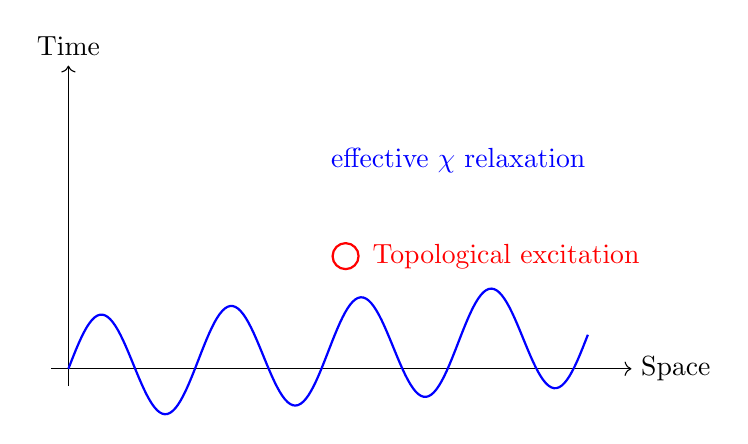
\begin{tikzpicture}[scale=1.1]

% Axes
      \draw[->] (-0.2,0) -- (6.5,0) node[right]{Space};
      \draw[->] (0,-0.2) -- (0,3.5) node[above]{Time};

% Wave
      \draw[thick, blue, domain=0:6, samples=200]
      plot (\x,{0.6*sin(2*pi*\x/1.5 r) + 0.4*\x/6});

% Particle crest
      \draw[red, thick] (3.2,1.3) circle (0.15);
      \node[red, right] at (3.4,1.3) {Topological excitation};

% Annotation
      \node[blue] at (4.5,2.4) {effective $\chi$ relaxation};

    \end{tikzpicture}
    \caption{Conceptual representation of Cosmochrony.
    An effective spacetime depiction of the projected scalar description of $\chi$,
      used for visualization purposes only.
      The monotonic relaxation of $\chi$ gives rise to an effective temporal ordering,
      while localized topological excitations correspond to particle-like configurations
      in the emergent geometric regime.}
    \label{fig:chi_concept}
  \end{figure}

  \paragraph{On the use of spacetime language.}
    Throughout this work, phrases such as ``spacetime coordinates,'' ``metric tensor,'' and ``four-dimensional
    manifold'' appear frequently, for the sake of clarity and effective description.
    These should be understood as \emph{emergent effective descriptions} valid in regimes where $\chi$
    has relaxed into a quasi-stable geometric configuration.
    They are not fundamental ingredients of the theory.

    At the deepest level, only $\chi$ and its internal relational variation structure exist.
    The appearance of familiar geometric language reflects the effectiveness of spacetime as a coarse-grained
    description of collective $\chi$
    behavior, analogous to how thermodynamic variables (temperature, pressure) emerge from molecular dynamics
    without those variables being fundamental.

    This interpretational stance is essential for distinguishing Cosmochrony from approaches that merely reformulate
    existing geometric theories in different variables.

  \subsection{The Geometric Effective Action and Lagrangians of Cosmochrony $\left(\mathcal{L}_{\mathrm{CC}}\right)$}
  \label{sec:geometric-action}

  \subsubsection*{Interpretational caution.}
    The action principle presented below employs conventional field-theoretic notation, including a metric tensor $g_{\mu \nu}$ and a four-dimensional integration measure. This should not be interpreted as assuming pre-existing spacetime structure.

    The formalism serves two purposes:
    \begin{enumerate}
      \item To provide a compact representation of $\chi$ dynamics in regimes where an effective spacetime description is valid.
      \item To establish the bridge between the fundamental relational network and the effective manifold description used in standard physics.
    \end{enumerate}

    The fundamental content of the theory is the field $\chi$ and its relaxation dynamics on a discrete graph. The metric $g_{\mu \nu}$ appearing in the action is a statistical emergent structure representing the connectivity and correlation density of the $\chi$ field, not an independent ontological input.

  \subsubsection*{Discrete Network Foundation}
    The dynamics of $\chi$ are fundamentally defined on a \textbf{discrete network}, where each node $i$ represents a local value $\chi_i$, and each link between nodes $i$ and $j$ is characterized by a \textbf{connectivity strength} $K_{ij}$. This matrix $K_{ij}$ encodes the correlation between neighboring $\chi$-values and serves as the microscopic foundation for the emergent geometry. In regimes where $\chi$ admits a quasi-stable geometric interpretation, $K_{ij}$ can be mapped to an effective metric $g_{\mu\nu}$ through the relation:
    \begin{equation}
      g_{\mu \nu} dx^\mu dx^\nu \approx \sum_{(u,v) \in \text{path}} \frac{1}{K_{uv}}
      \label{eq:metric-emergent}
    \end{equation}

  \subsubsection*{Explicit Form of the Connectivity Matrix $K_{ij}$}
    \label{subsec:Kij-definition}
    The connectivity strength $K_{ij}$ between nodes $i$ and $j$ encodes the \textbf{local correlation} between their respective $\chi$-field values. To ensure consistency with the emergent geometry and the dynamical constraints of the $\chi$ field, we adopt the following \textbf{constitutive relation}:
    \begin{equation}
      K_{ij} = K_0 \cdot f\left(\frac{|\chi_i - \chi_j|^2}{\chi_c^2}\right)
      \label{eq:Kij-def}
    \end{equation}
    where:
    \begin{itemize}
      \item $K_0$ is a \textbf{fundamental coupling scale} (with dimensions of $[\text{length}]^{-2}$), representing the maximal connectivity strength in regions where $\chi$ is uniform.
      \item $\chi_c$ is a \textbf{characteristic scale} of the $\chi$ field, naturally associated with the Planck length or the cosmological relaxation scale.
      \item $f(x)$ is a \textbf{dimensionless, monotonically decreasing function} satisfying $f(0) = 1$ and $f(x) \to 0$ as $x \to \infty$.
    \end{itemize}

    A physically motivated choice for $f(x)$ is:
    \begin{equation}
      f(x) = \frac{1}{1 + x}
    \end{equation}
    This ansatz ensures that:
    \begin{enumerate}
      \item \textbf{Symmetry}: $K_{ij} = K_{ji}$, as required for a consistent relational structure.
      \item \textbf{Locality}: $K_{ij}$ depends only on the \textbf{local difference} $|\chi_i - \chi_j|$, reflecting the pre-geometric nature of the $\chi$ field.
      \item \textbf{Boundedness}: $0 < K_{ij} \leq K_0$, preventing unphysical divergences in the emergent metric.
      \item \textbf{Gradient sensitivity}: $K_{ij}$ decreases as $|\chi_i - \chi_j|$ increases, encoding the \textbf{resistance to relaxation} induced by localized excitations (e.g., particles or curvature).
    \end{enumerate}

    This form of $K_{ij}$ provides a \textbf{microscopic foundation} for the emergent metric $g_{\mu\nu}$, as
    detailed in Section~\ref{subsec:emergent-metric}.
    The coupling scale $K_0$ and the characteristic scale $\chi_c$ are expected to be related to fundamental
    constants (e.g., the Planck length $\ell_P$ or the Hubble scale $H_0^{-1}$), but their precise values are left
    as phenomenological parameters to be constrained by observations (see Section~\ref{subsec:normalization-of-the-chi-field}).

  \subsubsection*{Emergent Geometry from $K_{ij}$}
    \label{subsec:emergent-metric}
    The connectivity matrix $K_{ij}$ defines an \textbf{operational distance} between nodes $i$ and $j$ via the minimal path sum:
    \begin{equation}
      d(i, j)^2 = \ell_0^2 \sum_{(u,v) \in \text{path}} \frac{1}{K_{uv}}
    \end{equation}
    where $\ell_0$ is a microscopic length scale (e.g., related to the Planck length).
    In the continuum limit, this discrete sum converges to the line element of an \textbf{emergent metric} $g_{\mu\nu}$:
    \begin{equation}
      ds^2 = g_{\mu\nu} dx^\mu dx^\nu \approx \ell_0^2 \left[ \delta_{\mu\nu} + \mathcal{O}\left(\frac{|\nabla \chi|^2}{\chi_c^2}\right) \right] dx^\mu dx^\nu
    \end{equation}
    Here, the corrections $\mathcal{O}(|\nabla \chi|^2 / \chi_c^2)$ encode the \textbf{curvature induced by localized excitations} (e.g., particles or black holes).
    This construction ensures that:
    \begin{itemize}
      \item \textbf{Flat spacetime} emerges when $\chi$ is uniform ($\nabla \chi = 0$), as $K_{ij} \approx K_0$ and $g_{\mu\nu} \approx \eta_{\mu\nu}$.
      \item \textbf{Curved spacetime} arises in regions where $\nabla \chi \neq 0$, as $K_{ij}$ varies spatially, inducing a non-trivial $g_{\mu\nu}$.
    \end{itemize}

    This mechanism provides a \textbf{geometric interpretation of gravity} as a modulation of the $\chi$-field's connectivity, without invoking a fundamental metric or curvature tensor.
    Further details on the continuum limit and the derivation of the effective field equations are provided in Appendix~\ref{sec:collective-coupling}.

  \subsubsection*{Effective action formulation.}
    In regimes where $\chi$ admits a quasi-stable geometric interpretation, the dynamics may be encoded in an effective action:
    \begin{equation}
      S_{\mathrm{CC}} = \int \mathcal{L}_{\mathrm{CC}} \sqrt{-g} \, d^4 x
    \end{equation}
    where the Lagrangian density decomposes as:
    \begin{equation}
      \mathcal{L}_{\mathrm{CC}} = \mathcal{L}_{\text{Gravity/Time}} + \mathcal{L}_{\chi / \text{Soliton}} + \mathcal{L}_{\text{Forces/Matter}}
    \end{equation}
    The symbol $\sqrt{-g}$ represents the invariant volume element. In regimes where no spacetime interpretation yet exists (e.g., at the nodes of the fundamental graph), this should be understood as an abstract integration measure $d\mu$ on the configuration space of $\chi$.

  \subsubsection*{Status of $g_{\mu\nu}$ in this formulation.}
    The metric $g_{\mu\nu}$ is an effective description of the coupling strengths $K_{ij}$ between $\chi$ nodes. It is defined by the requirement that the distance $ds^2$ in the continuum matches the operational distance derived from the network's connectivity:
    \begin{equation}
      g_{\mu\nu} dx^\mu dx^\nu \approx \sum_{(u,v) \in \text{path}} \frac{1}{K_{uv}}
    \end{equation}
    Consequently, $g_{\mu\nu}$ is a phenomenological summary of the underlying relational dynamics, capturing the local rate of $\chi$-relaxation and its spatial correlations.

  \subsection{Physical Interpretation}
  \label{subsec:physical-interpretation}

  In Cosmochrony, spacetime is not postulated as a fundamental background structure.
  Instead, it arises as an effective macroscopic description once configurations of
  the relational substrate $\chi$ admit a sufficiently stable and projectable regime.
  Temporal and spatial notions are therefore understood as emergent features of a
  single underlying irreversible ordering process, rather than as independent
  primitives.

  In such regimes, the infra-physical projection from $\chi$ to an effective
  description $\chi_{\mathrm{eff}}$ yields a factorisable structure, allowing an
  approximate decomposition into subsystems and the definition of operational
  observables.
  This factorisation underlies the emergence of classical locality, compatibility of
  measurements, and standard relativistic descriptions in stable domains, as
  illustrated in Fig.~\ref{fig:classical-factorisable}.

  \begin{figure}[t]
    \centering
    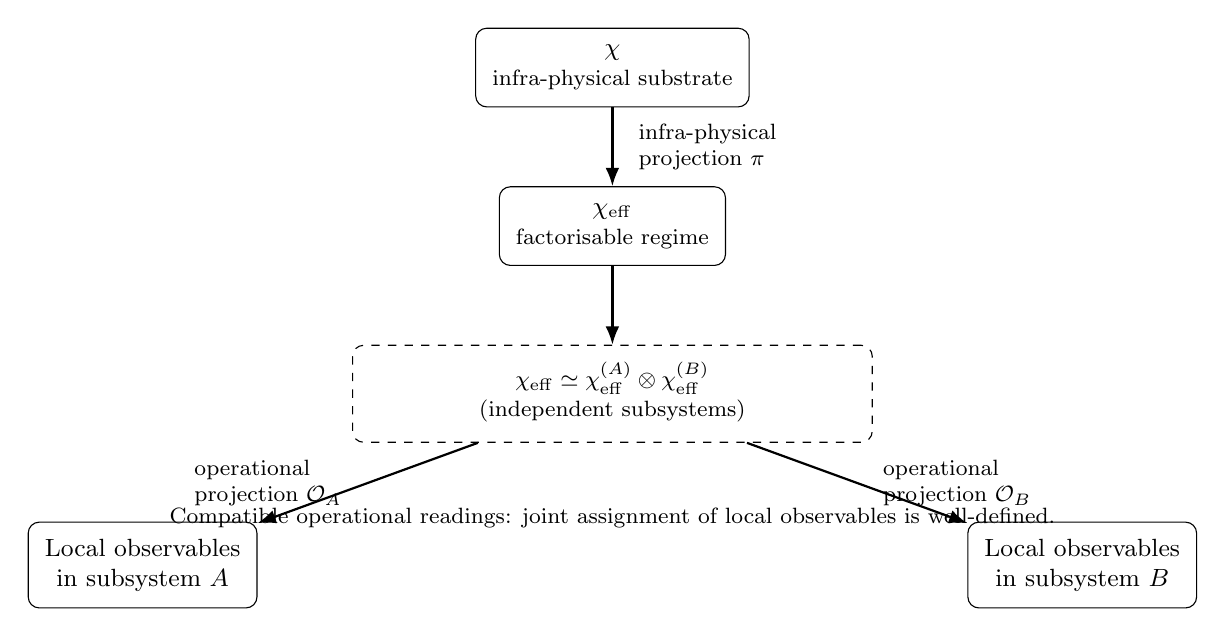
\begin{tikzpicture}[
      font=\small,
      node distance=10mm,
      box/.style={draw, rounded corners, align=center, inner sep=6pt},
      arrow/.style={-Latex, thick},
      note/.style={align=left, font=\footnotesize},
      dashedbox/.style={draw, dashed, rounded corners, inner sep=6pt}
    ]

    \node[box] (chi) {$\chi$\\\footnotesize infra-physical substrate};

    \node[box, below=of chi] (chieff) {$\chi_{\mathrm{eff}}$\\\footnotesize factorisable regime};

    \node[dashedbox, below=of chieff, minimum width=6.6cm] (decomp) {
      \begin{tabular}{c}
        \footnotesize $\chi_{\mathrm{eff}} \simeq \chi_{\mathrm{eff}}^{(A)} \otimes \chi_{\mathrm{eff}}^{(B)}$\\
        \footnotesize (independent subsystems)
      \end{tabular}
    };

    \node[box, below left=10mm and 12mm of decomp] (obsA) {Local observables\\in subsystem $A$};
    \node[box, below right=10mm and 12mm of decomp] (obsB) {Local observables\\in subsystem $B$};

    \draw[arrow] (chi) -- node[right=2mm, note] {infra-physical\\projection $\pi$} (chieff);
    \draw[arrow] (chieff) -- (decomp);

    \draw[arrow] (decomp) -- node[left=2mm, note] {operational\\projection $\mathcal{O}_A$} (obsA);
    \draw[arrow] (decomp) -- node[right=2mm, note] {operational\\projection $\mathcal{O}_B$} (obsB);

    \node[note, below=7mm of decomp, align=center] (compat)
    {\footnotesize Compatible operational readings: joint assignment of local observables is well-defined.};

    \end{tikzpicture}
    \caption{Classical (factorisable) regime.
    After the infra-physical projection $\pi$, the effective description
      $\chi_{\mathrm{eff}}$ admits an approximate decomposition into independent subsystems.
      Operational projections $\mathcal{O}_A$ and $\mathcal{O}_B$ then yield compatible local
      observables, recovering standard classical and relativistic descriptions.
      This figure illustrates the hierarchy between infra-physical projection and
      operational observation, and contrasts with the non-factorisable regimes discussed
      in later sections.}
    \label{fig:classical-factorisable}
  \end{figure}

  Because the projection from $\chi$ to $\chi_{\mathrm{eff}}$ is generically
  non-injective, the effective observables obtained in this way summarize relational
  structure without exhausting the underlying degrees of freedom.
  Distinct $\chi$ configurations may therefore correspond to identical effective
  descriptions, while a single underlying configuration may admit multiple correlated
  operational realizations.
  This structural asymmetry is central to the emergence of both classical and quantum
  phenomenology, and is developed in detail in subsequent sections.

  Within this interpretation, temporal ordering, relational separation, and large-scale
  behavior are not treated as independent postulates, but as complementary effective
  summaries of the same underlying relaxation dynamics, appearing at different levels
  of coarse-graining.
  Their precise operational and dynamical roles are introduced progressively in the
  following sections.

  The physical content of the theory thus resides entirely in the dynamics of the
  fundamental $\chi$ substrate, while spacetime notions function as emergent,
  context-dependent descriptive tools rather than as fundamental ingredients.

  \subsection{Relational Projection and Spectral Admissibility}
  \label{sec:relational_projection}

  In Cosmochrony, admissible physical descriptions are not defined by spacetime
  locality or geometric structure, but by the spectral properties of the relational
  substrate $\chi$.

  \paragraph{Relational operator.}
    Let $\mathcal{H}_\chi$ denote the configuration space of admissible $\chi$ states.
    We introduce a relational operator
    \begin{equation}
      L_\chi : \mathcal{H}_\chi \rightarrow \mathcal{H}_\chi,
    \end{equation}
    defined purely in terms of $\chi$ correlations.
    In discrete implementations (Appendix~D), $L_\chi$ reduces to a graph Laplacian
    associated with relational adjacency; in the continuum limit, it defines an
    effective self-adjoint operator encoding relational connectivity.

  \paragraph{Spectral decomposition.}
    The operator $L_\chi$ admits a spectral decomposition
    \begin{equation}
      L_\chi \psi_n = \lambda_n \psi_n,
    \end{equation}
    where $\{\lambda_n\}$ are non-negative eigenvalues and $\{\psi_n\}$ the associated
    eigenmodes.
    No geometric or spacetime interpretation is assumed at this stage.

  \paragraph{Admissibility as spectral filtering.}
    Projectable configurations are selected by a spectral filter acting on $L_\chi$.
    We define the infra-physical admissibility projection as
    \begin{equation}
      \Pi_{\lambda_*} \;\equiv\; f\!\left(\frac{L_\chi}{\lambda_*}\right),
    \end{equation}
    where $f(x)$ is a fixed, smooth cutoff function satisfying
    $f(x)\to 0$ for $x\ll 1$ and $f(x)\to 1$ for $x\gg 1$.
    The scale $\lambda_*$ sets the characteristic spectral threshold separating
    admissible from non-admissible relational modes.

    This construction defines admissibility without reference to spacetime,
    coordinates, or integration measures, relying solely on spectral properties
    of the relational operator.

  \subsection{Monotonicity and Arrow of Time}
  \label{subsec:monotonicity-and-arrow-of-time}

  A central structural postulate of Cosmochrony is that the relational substrate $\chi$
  admits an intrinsic, globally ordered relaxation structure.
  In effective descriptions, this ordering manifests as the monotonic behavior of the
  projected scalar descriptor $\chi_{\mathrm{eff}}$ along admissible ordering paths:
  \begin{equation}
    \mathcal{D}_{\lambda} \chi_{\mathrm{eff}} \ge 0 .
  \end{equation}
  Here $\lambda$ denotes an ordering parameter associated with the relaxation of
  projected $\chi$ configurations, rather than a fundamental time coordinate.
  The inequality expresses a structural constraint on admissible projected
  representations, not an evolution equation for a fundamental scalar quantity.

  This monotonicity reflects an intrinsic asymmetry in the ordering structure of $\chi$
  configurations.
  Because the projection from $\chi$ to $\chi_{\mathrm{eff}}$ is generically
  non-injective, admissible effective descriptions may lose information about
  underlying configurations, but cannot exhibit reversals of the ordering induced by
  relaxation.

  Within this framework, energy is interpreted as an effective measure of the
  remaining capacity of projected $\chi$ configurations to undergo further
  relaxation.
  As relaxation proceeds, this capacity is irreversibly expended in the projected
  description.
  Admissible ordering paths therefore exclude any effective decrease of
  $\chi_{\mathrm{eff}}$, which would correspond to a restoration of relaxation capacity
  incompatible with the underlying ordering structure.

  Irreversibility follows directly from this structural constraint.
  The arrow of time is identified with the directional ordering induced by relaxation:
  the progression from configurations with greater effective relaxation capacity
  toward configurations in which that capacity has been locally or globally exhausted.

  This temporal orientation is not derived from coarse-graining, entropy production,
  or special initial conditions.
  It arises prior to any statistical or thermodynamic description, as a direct
  consequence of the ordering constraints imposed by $\chi$ on its admissible
  projections.
  The relation to thermodynamic irreversibility is discussed further in
  Section~\ref{subsec:entropy-arrow}.

  \subsection{Local Relaxation Speed}
  \label{subsec:local-relaxation-speed}

  A fundamental structural constraint of the Cosmochrony framework is that the effective
  local ordering rate associated with projected $\chi$ configurations is bounded.
  In effective geometric descriptions, this constraint takes the form
  \begin{equation}
    \left| \mathcal{D}_{\mathrm{loc}} \chi_{\mathrm{eff}} \right| \le c ,
  \end{equation}
  where $\mathcal{D}_{\mathrm{loc}} \chi_{\mathrm{eff}}$ denotes an effective local
  relaxation functional characterizing the maximal admissible ordering of projected
  $\chi$ configurations.
  The constant $c$ is the effective causal bound observed in spacetime.

  This inequality expresses a constraint on admissible projected descriptions, not a
  propagation speed defined at the level of the $\chi$ substrate.
  It limits the maximal rate at which effective causal connectivity and local geometric
  relations can be established within descriptions compatible with the intrinsic
  ordering structure of $\chi$.
  The quantity $c$ therefore characterizes the causal structure of the projected regime
  rather than the dynamics of the pre-geometric substrate itself.

  Local particle propagation, signal transmission, and field interactions are all
  constrained by this bound in effective spacetime descriptions.
  By contrast, the underlying $\chi$ substrate is not subject to spacetime notions of
  velocity or signal propagation.

  Apparent superluminal recession velocities at cosmological scales arise from cumulative
  and global effects of projected $\chi$ ordering and do not violate this local causal
  constraint.
  Local causal relations remain bounded by $c$ in all admissible effective descriptions.

  \subsection{Relation to Conventional Fields}
  \label{subsec:relation-to-conventional-fields}

  Effective descriptions derived from projected $\chi$ configurations may formally
  resemble scalar or tensor fields used in cosmology and particle physics.
  This resemblance, however, reflects the emergence of a spacetime-based descriptive
  language, not the presence of an additional fundamental field.
  The $\chi$ substrate itself remains a pre-geometric relational structure, independent
  of spacetime and field-theoretic notions.

  Within Cosmochrony, energy and quantization are not fundamental attributes of $\chi$.
  They arise only at the effective level, as consequences of the non-injective
  projection from $\chi$ to admissible observables.
  Only certain stable, localized, and spectrally isolated configurations admit a
  particle-like interpretation and can be consistently described using conventional
  quantum field-theoretic tools in regimes where a spacetime description is valid.

  Matter, radiation, and interactions are therefore not associated with independent
  fundamental fields coupled to $\chi$.
  They correspond instead to effective degrees of freedom arising from structural
  constraints, spectral organization, and long-lived relational patterns of projected
  $\chi$ configurations.
  Standard Model fields are recovered as accurate effective descriptions within the
  appropriate coarse-grained regimes.

  From this perspective, Cosmochrony does not extend the Standard Model by introducing
  new fundamental fields.
  Rather, it provides an ontological explanation for the emergence, applicability, and
  structural properties of effective field descriptions themselves.

  \subsection{Initial Conditions and Global Structure}
  \label{subsec:initial-conditions-and-global-structure}

  The Cosmochrony framework does not postulate initial conditions in the conventional
  temporal sense.
  Instead, it assumes that the relational substrate $\chi$ admits a minimal admissible
  ordering state, denoted $\chi_0$, which defines a structural boundary of admissible
  projected descriptions.
  This state does not correspond to a distinguished moment in time, but to the earliest
  configurations for which an effective ordering interpretation becomes meaningful.

  In effective geometric regimes, the characteristic scale associated with projected
  descriptions in the vicinity of $\chi_0$ coincides numerically with the Planck scale.
  This correspondence reflects the breakdown of projectability and of coarse-grained
  spacetime descriptions below this regime, rather than the presence of a fundamental
  cutoff, microscopic discreteness, or underlying spacetime lattice.

  From this perspective, cosmic history is interpreted as the progressive and
  irreversible ordering of projected $\chi$ configurations away from this minimal
  admissible boundary.
  No spacetime singularity is required at the fundamental level.
  Apparent singular behavior arises only when classical notions of time, distance, or
  curvature are extrapolated beyond the regime in which projected $\chi$ configurations
  admit a stable geometric and causal interpretation.

  \paragraph{Ontological poverty and the growth of admissible structure.}
    The minimal admissible state $\chi_0$ corresponds to a regime of \emph{ontological
poverty}, as defined in Section~\ref{sec:definition-and-fundamental-properties-of-the-chi-field}.
    Only a severely restricted class of simple and highly coherent configurations can be
    projected in this regime.
    As relaxation proceeds, the space of admissible configurations expands, enabling the
    emergence of increasingly rich, localized, and hierarchical effective structures.
    This growth reflects an expansion of descriptive and relational capacity, rather than
    the unfolding of pre-encoded complexity.

    The global structure of admissible projected descriptions is therefore constrained by
    the ordering properties of the underlying $\chi$ substrate, rather than by arbitrarily
    specified initial data or boundary conditions.
    In the following section, we derive a minimal effective dynamical equation governing
    the ordering of projected $\chi$ configurations and explore its immediate physical
    consequences.


  \section{Dynamical Equation for the $\chi$ Field}
  \label{sec:dynamical-equation-for-the-chi-field}

  \subsection{Parameter-Independent Relaxation}
  \label{subsec:parameter-independent-relaxation}

  To avoid the conceptual pitfalls associated with a fundamental time coordinate,
  the dynamics of the scalar quantity $\chi$ is formulated without reference to any
  external temporal parameter.
  Instead, physical evolution is described as an ordered sequence of $\chi$
  configurations, denoted $(\chi_\lambda)$, where $\lambda$ is a strictly monotonic
  ordering parameter labeling the relaxation process.

  At the fundamental level, the dynamics of $\chi$ is defined by an intrinsic
  relaxation flow:
  \begin{equation}
    \mathcal{D}_{\lambda}\chi = \mathcal{R}[\chi],
  \end{equation}
  where $\mathcal{R}[\chi]$ denotes the local rate of relaxation toward equilibrium,
  defined purely in terms of the relational structure of $\chi$ configurations.
  No spacetime derivative or geometric operator is assumed at this stage.

  Quantities commonly interpreted as temporal derivatives arise only at the level of
  effective descriptions, when $\chi$ configurations admit a quasi-stable geometric
  interpretation.
  In such regimes, a coordinate time parameter may be introduced as a convenient
  label of the relaxation ordering, but it carries no fundamental significance and
  does not affect the underlying dynamics.

  Within this framework, relaxation does not occur \emph{in} time.
  Rather, the cumulative relaxation of $\chi$ defines what is operationally
  identified as physical duration.
  Local variations in the relaxation rate provide the effective measure of temporal
  flow, establishing a direct connection between the structure of $\chi$
  configurations and the emergent notion of time.

  \subsection{Hamiltonian Derivation of the Evolution Equation}
  \label{subsec:hamiltonian-derivation}

  While the dynamics of $\chi$ can be viewed as a minimal relaxation principle, it can be more rigorously derived from a
  Hamiltonian constraint.
  We postulate that the dynamics of $\chi$ are governed by a Dirac-type kinematic constraint in phase space, analogous
  to the mass-shell condition for a massless relativistic particle:
  \begin{equation}
  (\partial_t \chi)
    ^2 + |\nabla \chi|^2 = c^2,
    \label{eq:hamiltonian_constraint}
  \end{equation}
  where $c$ is the fundamental velocity scale.
  Combined with the \textit{arrow of time} postulate ($\partial_t \chi \geq 0$), which reflects the irreversible
  relaxation of the Cosmochron, this leads uniquely to the first-order evolution equation:
  \begin{equation}
    \partial_t \chi = c \sqrt{1 - \frac{|\nabla \chi|^2}{c^2}}.
    \label{eq:chi_dynamics}
  \end{equation}

  This derivation grounds the ``minimal principle'' in the symplectic structure of the field's phase space, ensuring
  that $\chi$ acts as an intrinsic time coordinate.

  The mathematical stability of this equation is demonstrated in~\ref{subsec:stability_chi}, while explicit analytical
  solutions are derived in~\ref{subsec:analytical_solutions_chi}.
  The coupling of the $\chi$ field with matter, extending this kinematic backbone to a dynamical theory, is further
  discussed in~\ref{subsec:coupling_matter_chi} and Section~\ref{subsec:variational-formulation}.

  \subsection{Microscopic Origin of the Coupling Tensor and the Poisson Equation}
  \label{subsec:microscopic-origin-of-the-coupling-tensor-and-the-poisson-equation}

  For internal consistency, the effective coupling governing the ordering of projected
  $\chi$ configurations cannot be treated as a fixed universal constant.
  Instead, it must depend on the internal structural state of the projected description,
  reflecting how localized configurations either facilitate or resist further relaxation.
  In Cosmochrony, this dependence is captured through a constitutive relation linking
  effective coupling strength to variations of the effective scalar descriptor
  $\chi_{\mathrm{eff}}$, without invoking any underlying spatial substrate or fundamental
  interaction at the pre-geometric level.

  A convenient phenomenological parametrization of this dependence is given by
  \begin{equation}
    K_{\mathrm{eff}}
    = K_0 \exp\!\left(
                  -\frac{(\Delta \chi_{\mathrm{eff}})^2}{\chi_c^2}
    \right),
    \label{eq:effective_coupling_tensor}
  \end{equation}
  where $\Delta \chi_{\mathrm{eff}}$ denotes a measure of effective internal variation
  between correlated projected configurations,
  $K_0$ characterizes the maximal relaxation conductivity in a homogeneous effective
  background, and $\chi_c$ sets the characteristic scale beyond which structural
  inhomogeneities significantly suppress relaxation efficiency.
  This expression should be understood as a constitutive relation for admissible projected
  descriptions, not as a fundamental law governing the $\chi$ substrate.

  Projected configurations exhibiting strong internal variation—such as stable solitonic
  or bound structures—therefore reduce the effective coupling and locally slow the
  admissible relaxation ordering.
  This reduction does not correspond to the introduction of a new interaction.
  It reflects instead the intrinsic resistance of structured projected configurations to
  further relaxation.
  The resulting slowdown provides the microscopic origin of the emergent gravitational
  phenomenology discussed in the preceding sections.

  In regimes where a spacetime description becomes applicable, the local effective
  relaxation rate $\mathcal{D}_{\mathrm{loc}} \chi_{\mathrm{eff}}$ differs from its
  asymptotic value $\mathcal{D}_0$ far from localized structures.
  An effective gravitational potential $\Phi$ may then be introduced as a descriptive
  parameter through the relation
  \begin{equation}
    \frac{\mathcal{D}_{\mathrm{loc}} \chi_{\mathrm{eff}}}{\mathcal{D}_0}
    \simeq 1 + \frac{\Phi}{c^2},
    \label{eq:relaxation_potential_relation}
  \end{equation}
  which summarizes the relative slowdown of effective relaxation ordering in a form
  familiar from classical gravitational phenomenology.
  The potential $\Phi$ has no independent ontological status and serves only as a compact
  parametrization of relaxation inhomogeneities.

  In the weak-structure regime, where effective internal variations remain small compared
  to $\chi_c$, the spatial distribution of $\Phi$ admits a simplified elliptic
  description.
  At this coarse-grained level, the effective dynamics reduce to a Poisson-type relation,
  \begin{equation}
    \nabla^2 \Phi \simeq 4\pi G_{\mathrm{eff}} \rho,
    \label{eq:effective_poisson_equation}
  \end{equation}
  where $\rho$ denotes the effective density of localized, relaxation-resistant projected
  configurations and $G_{\mathrm{eff}}$ is an emergent coupling parameter encoding the
  collective response of the relaxation ordering to such structures.
  Both quantities are defined strictly within the effective geometric description.

  This Poisson equation is not fundamental.
  It represents the weak-field, macroscopic limit of the constrained ordering of
  projected $\chi$ configurations, expressed in a form adapted to effective spacetime
  description.
  Gravitation therefore appears not as an independent interaction, but as a descriptive
  manifestation of reduced relaxation conductivity induced by structured projected
  configurations.

  A fully relational formulation, consistent with but not required for the effective
  description adopted here, is provided in
  Appendix~\ref{app:relational_formulation}.

  \paragraph{Status of effective equations.}
    The effective equations introduced in this subsection—

  \subsection{Variational Formulation and Born--Infeld Action}
  \label{subsec:variational-formulation}

  In regimes where projected $\chi$ configurations admit a stable geometric
  interpretation, the effective relaxation constraints introduced above may be
  summarized in a compact variational form.
  This formulation is not fundamental and does not define a dynamics of the
  pre-geometric $\chi$ substrate.
  Rather, it provides an auxiliary and regularized representation of admissible
  projected descriptions in the presence of localized relaxation-resistant
  configurations.

  Motivated by Born--Infeld--type non-linear actions, originally introduced to control
  field singularities and enforce upper bounds on physical gradients~\cite{BornInfeld1934,DeserGibbons1998}, we
  consider the effective Lagrangian density
  \begin{equation}
    \mathcal{L}_{\mathrm{eff}}
    = -c^2 \sqrt{1 - \frac{|\nabla \chi_{\mathrm{eff}}|^2}{c^2}}
    + \mathcal{D}_{\mathrm{loc}}\chi_{\mathrm{eff}}
    - \frac{4\pi G_{\mathrm{eff}}}{c^2}\,\rho\,\chi_{\mathrm{eff}} ,
    \label{eq:leff_equation}
  \end{equation}
  where $\chi_{\mathrm{eff}}$ denotes the effective scalar descriptor introduced in
  Sec.~\ref{subsec:geometric-action},
  $\mathcal{D}_{\mathrm{loc}}\chi_{\mathrm{eff}}$ is the effective local relaxation
  ordering defined in Sec.~\ref{subsec:parameter-independent-relaxation}, and $\rho$
  represents the effective density of localized, relaxation-resistant projected
  configurations.
  All quantities appearing in this expression are defined strictly within the effective
  geometric description.

  The linear dependence on $\mathcal{D}_{\mathrm{loc}}\chi_{\mathrm{eff}}$ enforces the
  monotonicity of admissible projected descriptions without introducing additional
  propagating degrees of freedom.
  The square-root structure acts as a non-linear regulator, ensuring that effective
  spatial variations remain bounded by the universal constraint $c$.
  This role is directly analogous to that of Born--Infeld electrodynamics, where the
  action enforces a maximal field strength without postulating new microscopic
  dynamics.

  Within this auxiliary variational framework, the Euler--Lagrange equation associated
  with $\chi_{\mathrm{eff}}$ reproduces the non-linear elliptic relation governing the
  spatial distribution of relaxation slowdown:
  \begin{equation}
    \nabla \cdot
    \left(
      \frac{\nabla \chi_{\mathrm{eff}}}
      {\sqrt{1 - |\nabla \chi_{\mathrm{eff}}|^2 / c^2}}
    \right)
    = \frac{4\pi G_{\mathrm{eff}}}{c^2}\,\rho ,
    \label{eq:nonlinear_poisson}
  \end{equation}
  which coincides with the effective Poisson-type relation obtained in
  Sec.~\ref{subsec:microscopic-origin-of-the-coupling-tensor-and-the-poisson-equation}.
  No new physical content is introduced at this stage; the variational formulation
  merely provides a compact and internally consistent encoding of the previously
  established constraints.

  This Born--Infeld--like action should therefore be understood strictly as an
  \emph{auxiliary variational representation}.
  It does not constitute a fundamental action principle, nor does it define equations
  of motion for the $\chi$ substrate.
  Its purpose is to regularize the effective description, enforce universal structural
  bounds, and facilitate comparison with standard gravitational phenomenology in the
  appropriate weak-field regime.

  The physical interpretation of this effective action is discussed in
  Appendix~\ref{subsec:hydrodynamic-limit}, while its mathematical consistency with the
  underlying relational dynamics and discrete formulation is established in
  Appendix~\ref{sec:born-lagrangian_derivation}.

\subsection{Why This Is Not a Scalar--Tensor Theory}
  \label{subsec:not-scalar-tensor}

  The effective variational formulation introduced in the previous subsection may
  superficially resemble scalar--tensor or modified gravity theories, in which a
  scalar field couples to geometry or mediates gravitational interactions.
  It is therefore essential to clarify that Cosmochrony does \emph{not} belong to this
  class of frameworks, either conceptually or technically.

  First, the effective scalar descriptor $\chi_{\mathrm{eff}}$ is \emph{not} a
  fundamental dynamical field.
  It does not represent an independent physical degree of freedom propagating on
  spacetime, nor does it possess intrinsic values or conjugate momenta.
  By construction, $\chi_{\mathrm{eff}}$ is a projected, coarse-grained descriptor of
  relational features of the pre-geometric substrate $\chi$, defined only in regimes
  where a spacetime interpretation becomes applicable.
  There is therefore no scalar field at the fundamental level whose dynamics could be
  coupled to geometry.

  Second, no modification of the gravitational sector is postulated.
  The metric appearing in effective descriptions is not an independent dynamical field,
  nor is it sourced or altered by a scalar field equation.
  Instead, geometric quantities summarize correlations between projected
  $\chi_{\mathrm{eff}}$ configurations.
  The Born--Infeld--like variational form introduced earlier does not define a new
  gravitational theory; it merely encodes, in a compact and regularized manner, the
  constraints governing admissible projected descriptions.
  In particular, there is no scalar--tensor coupling term of the form
  $f(\chi_{\mathrm{eff}}) R$, nor any modification of the Einstein--Hilbert action.

  Third, the effective equations derived from the auxiliary variational formulation do
  not introduce additional propagating modes.
  In scalar--tensor theories, the scalar field typically carries its own dynamics,
  leading to extra degrees of freedom, modified wave propagation, or additional
  polarization states.
  In Cosmochrony, by contrast, $\chi_{\mathrm{eff}}$ does not propagate independently.
  All effective equations constrain admissible relaxation patterns of projected
  configurations and do not enlarge the physical phase space.

  Finally, the origin of gravitational phenomenology in Cosmochrony is fundamentally
  different.
  Gravitation does not arise from the exchange of a scalar mediator or from a dynamical
  coupling between scalar and tensor sectors.
  It emerges instead from the local inhibition of relaxation ordering induced by
  structured projected configurations.
  The appearance of Poisson-like equations or gravitational potentials reflects the
  weak-structure limit of this constrained ordering, not the presence of a scalar
  gravitational field.

  In summary, Cosmochrony should not be interpreted as a scalar--tensor or modified
  gravity theory.
  The effective scalar descriptor $\chi_{\mathrm{eff}}$ is neither fundamental nor
  dynamical, the variational formulation is auxiliary rather than postulatory, and no
  additional gravitational degrees of freedom are introduced.
  The framework therefore avoids the conceptual and phenomenological issues commonly
  associated with scalar--tensor theories, while reproducing standard gravitational
  behavior in the appropriate effective regimes.

  \subsection{Causality and Locality}
  \label{subsec:causality-and-locality}

  Equation~\eqref{eq:chi_dynamics} does not define a fundamental dynamics of the
  $\chi$ substrate.
  Rather, it constrains admissible projected descriptions in regimes where a
  geometric interpretation becomes applicable.
  Within such effective descriptions, the relaxation ordering encoded by
  $\chi_{\mathrm{eff}}$ exhibits locality and causality in the operational sense
  relevant to physical observables.

  Effective locality follows from the fact that variations of
  $\chi_{\mathrm{eff}}$ at a given effective spacetime event depend only on
  correlated neighboring projected configurations, as defined within the emergent
  geometric description.
  No instantaneous coupling, action at a distance, or nonlocal influence is
  introduced at the level of effective physical observables.
  All admissible projected descriptions therefore respect locality in the sense
  appropriate to an emergent spacetime framework.

  Causality is enforced through the existence of a universal bound on the effective
  local relaxation ordering,
  \[
    \left| \mathcal{D}_{\mathrm{loc}} \chi_{\mathrm{eff}} \right| \le c ,
  \]
  which constrains the maximal rate at which correlations between effective
  configurations may be established.
  This bound functions as an effective causal constraint without presupposing a
  fundamental spacetime structure, lightcones, or signal propagation at the level
  of the $\chi$ substrate.

  Within effective physical descriptions, no superluminal propagation of signals
  or causal influence occurs.
  Apparent superluminal recession velocities observed in cosmological contexts
  arise solely from the cumulative integration of locally constrained relaxation
  ordering over extended regions.
  They therefore remain fully consistent with effective locality and causality as
  defined within the Cosmochrony framework.

  \medskip
  \noindent\emph{Conceptual remark.}—
  The effective causal bound $c$ introduced here should not be interpreted as an
  independent physical postulate.
  As established in Section~\ref{subsec:role-of-cchi}, it corresponds to the
  projected manifestation of the invariant structural bound $c_\chi$ defined at
  the level of the pre-temporal $\chi$ substrate.
  In regimes admitting a locally injective projection and a stable geometric
  interpretation, $c_\chi$ acquires an operational meaning as a maximal admissible
  local ordering rate, which appears in spacetime descriptions as the effective
  causal constraint $c$.

  Effective causality in Cosmochrony thus arises as a derived property of bounded
  projective realizations, rather than as a fundamental principle imposed on
  spacetime itself.

  \subsection{Homogeneous Cosmological Limit}
  \label{subsec:homogeneous-cosmological-limit}

  In a homogeneous and isotropic regime, projected $\chi$ configurations exhibit no
  effective spatial variations.
  The admissible relaxation ordering is then uniform across the emergent description,
  and the effective local relaxation rate attains its maximal allowed value,
  \begin{equation}
    \mathcal{D}_{\mathrm{loc}}\chi_{\mathrm{eff}} = c ,
  \end{equation}
  where $c$ denotes the universal bound constraining effective relaxation ordering.

  When expressed in terms of an effective cosmological time parameter $t$, introduced
  solely as a convenient label of the relaxation ordering, this uniform regime may be
  represented by the linear relation
  \begin{equation}
    \chi_{\mathrm{eff}}(t) = \chi_{\mathrm{eff},0} + c\, t ,
  \end{equation}
  where $\chi_{\mathrm{eff},0}$ denotes a reference value fixing the origin of the
  effective description.
  This parametrization does not introduce a fundamental time variable, nor does it
  assign intrinsic values to the $\chi$ substrate.
  It serves only as a compact representation of cumulative relaxation ordering in a
  homogeneous cosmological regime.

  Interpreting effective spatial distances as accumulated relational differentiation
  between projected configurations, this uniform ordering directly leads to a
  Hubble-like expansion law, as discussed in Sec.~\ref{sec:cosmology}.
  Cosmic expansion thus reflects the global ordering of projected $\chi$
  configurations, rather than the presence of an external energy component or a
  fundamental expansion of spacetime itself.

  As shown in Appendix~\ref{subsec:minimal-kinematic-constraint}, the requirement that
  effective relaxation ordering remain monotonic in an expanding regime implies the
  existence of a minimal residual structural inhomogeneity in projected $\chi$
  configurations.
  In effective geometric terms, this manifests as a non-vanishing lower bound on
  gravitational acceleration, providing a natural explanation for MOND-like
  phenomenology without invoking dark matter particles~\cite{FamaeyMcGaugh2012}.

  \subsection{Influence of Local Structure}
  \label{subsec:influence-of-local-structure}

  In regions where projected $\chi$ configurations exhibit non-vanishing effective
  structural variations, the admissible local relaxation ordering is reduced.
  This slowdown plays a central role in the emergence of gravitational phenomena
  within the Cosmochrony framework.

  Localized relaxation-resistant configurations—describable in effective regimes as
  particle-like solitonic structures—act as constraints on the admissible ordering of
  projected $\chi$ configurations.
  By increasing the effective structural complexity of the projected description,
  they reduce the local effective relaxation rate without introducing any additional
  interaction or force.

  When a geometric description becomes applicable, this mechanism manifests
  phenomenologically as gravitational time dilation and spatial curvature.
  No independent gravitational field is postulated.
  Gravitation emerges instead as a collective consequence of locally constrained
  effective relaxation ordering, reflecting the presence of structured projected
  configurations.

  \subsection{Unified Origin of Geometric and Field Effects}
  \label{subsec:unified-origin}

  The relationship between the $\chi$ substrate and the effective spacetime metric
  $g_{\mu\nu}$ is strictly hierarchical, reflecting the transition from a fundamental
  pre-geometric relational structure to smooth geometric descriptions applicable at
  macroscopic scales.

  \begin{enumerate}
    \item \textbf{Primacy of the $\chi$ substrate:}
    At the fundamental level, physical reality is described solely in terms of the
    $\chi$ substrate and its intrinsic relational structure.
    The $\chi$ substrate is not defined on spacetime, does not possess numerical
    values, and is not governed by a dynamical field equation.
    Ordering, relaxation, and causal notions arise only at the level of admissible
    projected descriptions.

    \item \textbf{Emergent Geometry:}
    In regimes where projected $\chi$ configurations admit a stable, slowly varying
    description, geometric notions become meaningful.
    The spacetime metric $g_{\mu\nu}$ arises as an effective descriptor summarizing the
    correlations and relaxation ordering of projected $\chi$ configurations.
    It provides a coarse-grained geometric language suitable for macroscopic
    observers, without acquiring independent ontological status.

    \item \textbf{Unified Interpretation of Fields and Gravitation:}
    Within this effective geometric description, localized relaxation-resistant
    projected configurations—describable as solitonic structures—are identified with
    matter degrees of freedom.
    Gravitational phenomena correspond to the local modulation of effective relaxation
    ordering induced by such structures.
    The metric does not act as an independent dynamical agent, but encodes the
    collective geometric response associated with constrained projected descriptions.
  \end{enumerate}

  In this framework, no independent gravitational interaction or fundamental field is
  postulated.
  Matter, geometry, and gravitational phenomena emerge as complementary aspects of the
  same constrained ordering of projected $\chi$ configurations, ensuring a unified and
  internally consistent description across scales.

  \subsection{Limitations and Scope}
  \label{subsec:limitations-and-scope}

  Equation~\eqref{eq:chi_dynamics} is intentionally minimal.
  It does not aim to provide a complete description of quantum fluctuations of
  $\chi$, nor does it incorporate higher-order backreaction effects.
  Its role is to capture the essential kinematic constraint governing the
  relaxation of $\chi$ in regimes where an effective geometric interpretation
  applies.

  Within this scope, the equation provides a unified backbone from which
  gravitational, quantum, and cosmological phenomena can be consistently
  \emph{recovered} or \emph{described} at an effective level, rather than derived
  from first principles.
  More refined treatments of fluctuations, correlations, and non-local structures
  lie beyond the present formulation and motivate further developments of the
  framework.

  In the following sections, this dynamical structure is applied to particles,
  gravitation, and entanglement, where its explanatory power can be directly
  assessed.


  \section{Particles as Localized Excitations of the $\chi$ Field}
  \label{sec:particles-as-localized-excitations-of-the-chi-field}

  \subsection{Particles as Stable Wave Configurations}
  \label{subsec:particles-as-stable-wave-configurations}

  Within the Cosmochrony framework, particles are not fundamental point-like objects.
  They arise only at the level of effective descriptions, as stable and localized
  configurations within projected $\chi$ descriptions.
  These configurations correspond to persistent patterns that locally constrain the
  admissible relaxation ordering, rather than to elementary entities propagating on a
  pre-existing spacetime background.

  In effective geometric regimes, such structures may be described using a wave-like
  or soliton-like language.
  They preserve their identity under interactions and effective displacement, while
  remaining entirely embedded in the constrained ordering of projected $\chi$
  configurations.
  Their apparent propagation reflects a continuous reconfiguration of admissible
  projected descriptions, not the motion of an object through a fundamental spacetime.

  In this sense, particle-like behavior does not originate from intrinsic degrees of
  freedom of the $\chi$ substrate.
  It emerges instead as a stable invariant of the effective relational structure once
  a spacetime interpretation becomes meaningful.

  \subsection{Topological Stability}
  \label{subsec:topological-stability}

  The stability of particle-like excitations is attributed to topological constraints rather than to conserved
  charges postulated a priori\cite{rajaraman1982solitons}.
  Nontrivial phase winding, torsion, or knot-like structures in $\chi$
  prevent continuous deformation into the vacuum state.

  Such topological protection naturally explains the discreteness of particle species and their robustness under
  perturbations.

  For instance, an electron corresponds to a localized knot in $\chi$
  with a specific winding number, where the knot's energy (proportional to its curvature) determines the
  particle's mass, and its topological charge (e.g., $4\pi$-periodicity) determines its spin-1/2 nature.

  The stability of solitonic excitations arises from a balance between the nonlinear self-interaction term $V(\chi)$
  (which tends to localize the field) and the gradient energy $|\nabla \chi|^2$
  (which tends to disperse it).
  Topological invariants, such as the winding number $n = \frac{1}{2\pi} \oint \nabla \arg(\chi) \cdot d\mathbf{l}$,
  further protect these configurations from decay, ensuring their persistence as particle-like objects.

  More topological configurations are discussed in ~\ref{subsec:topological_solitons}

  \subsection{Mass as Resistance to $\chi$ Relaxation}
  \label{subsec:mass_as_resistance}

  In Cosmochrony, mass is not introduced as an intrinsic or fundamental property of matter.
  Instead, it emerges as a quantitative measure of how strongly a localized configuration of
  the $\chi$ field resists the global relaxation flow.

  A particle-like excitation is modeled as a stable, localized solitonic configuration
  $\chi_s$, characterized by sustained internal structure and non-vanishing gradients.
  Such configurations locally inhibit the relaxation of $\chi$, producing a slowdown
  relative to the homogeneous background evolution. In an effective geometric description,
  this slowdown manifests as inertial persistence and gravitational time dilation.

  We define the structural energy associated with a solitonic configuration $\chi_s$ as
  the excess relaxation capacity stored in its internal curvature:
  \begin{equation}
    E[\chi_s] \;\equiv\;
    \int_{\Sigma}
    \left(
      \frac{1}{\sqrt{1 - |\nabla \chi_s|^2 / c^2}} - 1
    \right)
    \, d\Sigma ,
    \label{eq:chi_soliton_energy}
  \end{equation}
  where $\Sigma$ denotes a hypersurface of constant effective ordering parameter,
  and $|\nabla \chi_s|$ quantifies the local structural deformation of the $\chi$ field.
  This expression measures the energetic cost of maintaining a non-relaxed configuration
  embedded within a globally relaxing substrate.

  The inertial mass associated with the soliton is then defined operationally as
  \begin{equation}
    m \;\equiv\; \frac{E[\chi_s]}{c^2}.
    \label{eq:mass_definition}
  \end{equation}

  This relation is not postulated but follows directly from the role of $E[\chi_s]$ as
  a measure of resistance to $\chi$ relaxation. The universal constant $c$ appears as
  the maximal relaxation rate of the field and therefore provides the unique conversion
  factor between relaxation energy and inertial response.

  Within this framework, the relation $E = mc^2$ is interpreted as a kinematic identity:
  mass quantifies the amount of relaxation potential locally trapped in a persistent
  $\chi$ configuration, while energy measures the same quantity expressed in relaxation units.

  In this sense, mass is not an independent attribute of matter, but a derived property
  encoding how strongly a localized $\chi$ configuration resists the irreversible
  relaxation that defines physical time.

  The question of how different particle masses arise from distinct solitonic
  configurations is addressed in Appendix~\ref{app:topological_solitons}, where a spectral characterization
  of $\chi$-field stability modes is proposed as the geometric origin of mass hierarchies.

  \subsection{Energy--Frequency Relation}
  \label{subsec:energy-frequency-solitons}

  The energy associated with a particle-like excitation is linked to the internal
  oscillation rate of its $\chi$ configuration.
  Within the Cosmochrony framework, this rate characterizes how strongly a localized
  structure resists relaxation: configurations with more rapid internal
  reorganization correspond to tighter localization and a greater capacity to
  store relaxation potential.

  This provides an effective interpretation of the relation
  \begin{equation}
    E \propto \nu ,
  \end{equation}
  in which energy measures the amount of relaxation potential trapped in a given
  configuration, while the frequency $\nu$ quantifies the characteristic rate at
  which this potential is internally redistributed.
  The frequency should not be interpreted as oscillation with respect to a
  fundamental time parameter, but as an intrinsic property of the excitation,
  which admits a temporal interpretation only at the effective geometric level.

  Within this perspective, Planck's constant emerges as an effective proportionality
  factor relating energy and frequency, determined by the intrinsic scales and
  coupling properties of the $\chi$ field.
  Its apparent universality reflects the robustness of these underlying scales
  across stable configurations, rather than the postulation of a fundamental
  quantization constant.

  A more explicit derivation of this relation, in the context of radiation and
  photon-like excitations of the $\chi$ field, is presented in
  Sec.~\ref{subsec:energy-frequency-radiation}.

  \subsection{Fermions and Bosons}
  \label{subsec:fermions-and-bosons}

  Within the Cosmochrony framework, particle statistics arise from the internal
  topological structure of localized $\chi$ excitations rather than from
  postulated quantum rules.
  Distinct classes of excitations are characterized by how their internal
  configuration responds to continuous rotations in configuration space.

  Configurations that require a $4\pi$ internal phase rotation to return to an
  equivalent state exhibit fermion-like behavior, while configurations that are
  $2\pi$-periodic correspond to boson-like excitations.
  This distinction reflects a fundamental topological property of the underlying
  $\chi$ configuration, not a feature imposed by external symmetry principles.

  In effective descriptions, such $4\pi$-periodic configurations may be associated
  with non-orientable or twisted internal structures, while $2\pi$-periodic
  configurations correspond to orientable ones.
  This provides a natural qualitative explanation for the spin--statistics
  connection, without introducing additional quantum postulates at the
  fundamental level.

  As throughout this work, references to phase rotations or periodicity should be
  understood as properties of the internal configuration space of $\chi$.
  Geometric representations of these structures are effective and illustrative,
  and do not imply the existence of a fundamental spatial manifold.

  \subsection{Spin as a Topological Property of $\chi$ Configurations}
  \label{subsec:spin_topology}

  Within the Cosmochrony framework, spin is not introduced as an intrinsic kinematic
  degree of freedom, nor as a consequence of spacetime symmetries.
  Instead, it emerges as a purely topological property of localized $\chi$ configurations.

  Certain stable solitonic excitations of the $\chi$ field possess an internal structure
  that cannot be continuously deformed to the vacuum configuration.
  These excitations are characterized by a non-trivial topology in their internal
  configuration space, independently of any background spatial geometry.

  In particular, a class of fermionic configurations requires a $4\pi$ internal rotation
  to return to an equivalent configuration.
  A $2\pi$ rotation corresponds to a non-contractible loop in the configuration space
  of $\chi$, while a $4\pi$ rotation is homotopic to the identity.
  Formally, this implies that the relevant configuration space admits a double covering,
  with fundamental group
  \begin{equation}
    \pi_1(\mathcal{C}_\chi) = \mathbb{Z}_2 ,
  \end{equation}
  where $\mathcal{C}_\chi$ denotes the space of admissible localized $\chi$ configurations.

  When an effective quantum description becomes applicable, localized $\chi$ excitations
  are represented by complex wavefunctions encoding the phase structure of underlying
  field fluctuations.
  For topologically non-trivial configurations, a $2\pi$ effective rotation induces
  a sign change of the associated wavefunction,
  \begin{equation}
    \psi \;\longrightarrow\; -\psi ,
  \end{equation}
  while a $4\pi$ rotation restores the original state.

  This behavior identifies such excitations as spin-$\tfrac{1}{2}$ fermions.
  Importantly, the appearance of a spinorial phase does not rely on a fundamental
  representation of the rotation group, but follows from the topological structure
  of the underlying $\chi$ configuration itself.

  The fermionic statistics of these excitations arises from the same topological origin.
  Two identical fermionic solitons correspond to configurations that share a common
  $\chi$-field topology and therefore cannot be continuously merged into a single
  configuration without violating field continuity.

  Exchanging two identical fermionic excitations corresponds topologically to a
  $2\pi$ rotation in the combined configuration space.
  As this operation induces a sign change of the effective wavefunction, symmetric
  configurations are dynamically forbidden.
  This provides a geometric and topological origin of the Pauli exclusion principle
  within the Cosmochrony framework~\cite{Pauli1925}.

  In Cosmochrony, spin and fermionic statistics are not postulated quantum properties,
  but manifestations of topological obstructions in the space of localized $\chi$
  configurations.
  The $4\pi$ periodicity, spin-$\tfrac{1}{2}$ behavior, and exclusion principle thus
  share a common geometric origin.

  \subsection{Antiparticles}
  \label{subsec:antiparticles}

  Within the Cosmochrony framework, antiparticles are not interpreted as independent
  fundamental entities or as excitations propagating backward in time.
  They arise, at the level of effective descriptions, as relationally conjugate
  counterparts of particle-like projected configurations.

  A particle and its antiparticle correspond to projected configurations belonging to
  distinct but conjugate topological classes within the space of admissible projected
  descriptions.
  These classes are related by an internal reversal of relational structure rather
  than by an inversion of a fundamental dynamical variable.

  Annihilation processes occur when a particle-like projected configuration and its
  conjugate combine into a composite projected description that no longer supports
  localized structural constraints.
  Such a configuration admits a continuous deformation toward a more homogeneous
  effective description, in which localized relaxation resistance disappears.

  In effective geometric and quantum descriptions, this transition manifests as the
  conversion of particle–antiparticle structure into delocalized radiation-like
  projected excitations.
  No fundamental structure is destroyed in this process.
  The underlying relational substrate remains intact, while localized topological
  organization is redistributed into admissible projected configurations with extended
  support.

  In this sense, particle–antiparticle annihilation does not represent the destruction
  of matter, but a reorganization of effective relational structure from localized to
  delocalized forms within the space of admissible descriptions.

  \subsection{Particle Creation and Destruction}
  \label{subsec:particle-creation-and-destruction}

  Within the Cosmochrony framework, particle creation does not correspond to the
  appearance of new fundamental entities.
  It arises at the level of effective descriptions, when a projected configuration
  acquires sufficient structural organization to support a stable, localized
  topological class.
  Such configurations become identifiable as particle-like only once a spacetime
  interpretation becomes meaningful.

  Particle creation therefore reflects the emergence of a new admissible projected
  description with persistent localization and relaxation resistance.
  This process does not involve the generation of structure at the level of the
  $\chi$ substrate, but a reorganization of admissible projected configurations within
  the space of effective descriptions.

  Conversely, particle destruction does not represent the annihilation of a
  fundamental object.
  It occurs when a previously localized projected configuration loses its topological
  admissibility or stability class.
  In such cases, the configuration can no longer sustain localized relaxation
  constraints and admits a continuous deformation toward a more delocalized effective
  description.

  In effective geometric and quantum regimes, this transition manifests as the
  conversion of particle-like projected configurations into extended, radiation-like
  descriptions.
  Creation and destruction thus reflect changes in the organization and admissibility
  of projected descriptions, rather than the appearance or disappearance of
  fundamental entities.

  Within this perspective, particles are not primitive ontological constituents.
  They are stable descriptive regimes of the relational substrate, whose formation
  and dissolution correspond to transitions between distinct classes of admissible
  projected configurations.

  \subsection{Summary}
  \label{subsec:summary7}

  Within the Cosmochrony framework, particles are not fundamental entities.
  They emerge only at the level of effective descriptions, as stable and localized
  projected configurations that resist admissible relaxation ordering.
  Their physical properties are not postulated but arise as invariants of the
  structural and topological organization of admissible projected descriptions.

  Mass is identified with the degree of effective relaxation resistance encoded in a
  localized projected configuration.
  It quantifies how strongly such a configuration constrains admissible relaxation
  ordering relative to a homogeneous effective background.
  In regimes where a relativistic description applies, this interpretation naturally
  leads to the relation $E = mc^2$, understood as a kinematic identity rather than a
  fundamental postulate.

  Spin and statistical behavior originate from topological obstructions in the space
  of admissible projected configurations.
  Fermionic configurations exhibit a $4\pi$ periodicity in configuration space, such
  that a $2\pi$ rotation corresponds to a non-contractible loop and induces a sign
  change of the effective wavefunction.
  This topological structure provides a common origin for spin-$\tfrac{1}{2}$
  behavior, fermionic antisymmetry, and the Pauli exclusion principle
  without invoking additional quantum axioms.

  Within this perspective, different particle attributes correspond to distinct
  topological invariants of admissible projected descriptions.
  Spin is associated with non-trivial covering properties of configuration space,
  while electric charge may be interpreted, at an effective level, as an oriented
  topological defect or vortex-like structure within projected descriptions.
  These attributes remain conceptually distinct but arise from a common relational
  substrate once a geometric interpretation becomes meaningful.

  Taken together, these results provide a unified account of particle properties
  compatible with both relativistic and quantum phenomenology, without introducing
  particles or their attributes as fundamental ontological constituents.
  Particles appear instead as stable descriptive regimes of the underlying relational
  structure, whose properties reflect the topology of admissible projected
  configurations.


  \section{Gravity as a Collective Effect of Particle Excitations}
  \label{sec:gravity-as-a-collective-effect-of-particle-excitations}

  \subsection{Local Slowdown of $\chi$ Relaxation}
  \label{subsec:local-slowdown-of-chi-relaxation}

  In cosmochrony, gravity does not arise from a fundamental interaction but from the collective influence of
  particle excitations on the dynamics of the $\chi$ field.
  As established in the previous section, localized excitations resist the local relaxation of $\chi$.

  When many such excitations are present, their effects superpose, leading to a macroscopic reduction of the
  relaxation rate:
  \begin{equation}
    \partial_t \chi = c \left( 1 - \alpha \rho \right),
  \end{equation}
  where $\rho$ denotes the effective density of particle excitations and $\alpha$
  is a coupling parameter encoding their influence on $\chi$.

  The coupling parameter $\alpha$ in $\partial_t \chi = c(1 - \alpha \rho)$
  is determined by the interaction strength between $\chi$
  and localized excitations. For a point-like excitation of mass $m$, $\alpha$ scales as $\alpha \sim G m / c^2$
  , where $G$ emerges as an effective coupling constant linking matter density to $\chi$
  -relaxation slowing. This yields the Newtonian potential $\Phi \sim \alpha \rho$ in the weak-field limit.

  This slowdown manifests physically as gravitational time dilation.

  \subsection{Collective Gravitational Coupling and Operational Geometry}
  \label{subsec:collective-gravitational-coupling-and-operational-geometry}

  The collective slowdown of $\chi$ relaxation described above not only affects the local flow of
  time but also induces an effective spatial coupling between neighboring regions of the field.
  When particle excitations are present, the resistance they impose on the relaxation of $\chi$
  modulates how efficiently variations of the field propagate across space.

  This collective behavior can be encoded in an effective local coupling between neighboring
  degrees of freedom, denoted $K_{ij}$, which characterizes the stiffness of the $\chi$ field to
  relative variations.
  In regions where $\chi$ varies smoothly, the coupling approaches a constant
  vacuum value, while strong local gradients associated with particle excitations effectively weaken
  the coupling.
  Importantly, $K_{ij}$ is assumed to be purely local and constitutive, depending only
  on neighboring values of $\chi$, rather than on any pre-existing spatial metric.

  Because no background geometry is assumed at the fundamental level, spatial distance is defined
  operationally through the propagation of $\chi$ across the network: two points are considered
  close if $\chi$-relaxation propagates efficiently between them, and distant otherwise. In the
  continuum and weak-gradient limit, this operational notion induces an effective spatial geometry,
  which can be described by a metric to leading order.

  In this sense, spacetime curvature in Cosmochrony does not arise as a primitive geometric property,
  but as a collective manifestation of how localized particle excitations modulate the propagation
  and relaxation of the $\chi$ field.

  The explicit construction of the collective coupling $K_{ij}$, the operational definition of
  distance on the discrete network, and the derivation of the effective field equations in the
  quasi-static regime are presented in Appendix~\ref{subsec:collective-coupling}.

  \subsection{Emergent Curvature}
  \label{subsec:emergent-curvature}

  Spatial variations in admissible relaxation ordering, combined with the collective
  modulation of effective coupling strength, lead to non-uniform correlation patterns
  within projected descriptions.
  When a smooth geometric parametrization becomes applicable, these non-uniformities
  are compactly summarized by gradients of an emergent metric structure.

  In Cosmochrony, spacetime curvature is therefore not a primitive geometric property
  nor the manifestation of an independent dynamical field.
  It is a descriptive construct encoding how localized projected configurations
  collectively modulate admissible ordering and correlation structure across extended
  regions.
  The metric does not act as a causal agent; it functions as a macroscopic summary of
  constrained relational organization within admissible projected descriptions.

  Within effective geometric regimes, this emergent curvature reproduces the
  phenomenology traditionally attributed to curved spacetime in general relativity,
  including gravitational time dilation, geodesic deviation, and lensing effects.
  These phenomena arise here not from a fundamental spacetime geometry, but from the
  spatial variation of admissible relaxation ordering and correlation efficiency.

  Crucially, this interpretation remains fully compatible with the pre-geometric and
  relational foundations of the framework.
  Geometry appears only as an effective and operational language, valid in regimes
  where projected $\chi$ configurations admit a smooth and slowly varying
  representation.

\paragraph{Einstein’s Equations as a Structural Equilibrium Principle}
  \label{subsec:einstein-equilibrium-principle}

  Within the Cosmochrony framework, Einstein’s field equations retain their full
  conceptual and physical legitimacy.
  They are not reinterpreted as approximations to a deeper gravitational dynamics,
  but as an exact and universal description of spacetime structure \emph{whenever a
geometric description is applicable}.

  This perspective is fully aligned with Einstein’s own methodological stance.
  General relativity does not describe the microscopic constitution of spacetime, but
  the necessary relations between geometry and physical content once spacetime itself
  is admitted as a meaningful concept.
  In this sense, Einstein’s equations are already formulated at the correct
  descriptive level: that of emergent geometry.

  In Cosmochrony, spacetime geometry is not assumed a priori, but arises from the
  admissible projection of the pre-geometric relational substrate $\chi$.
  When projected $\chi$ configurations admit a smooth, locally injective geometric
  description, their collective structural constraints can be summarized by an
  effective metric $g_{\mu\nu}$.
  In this regime, Einstein’s equations emerge \emph{necessarily} as the unique
  consistency condition relating curvature to the effective distribution of
  relaxation-resistant configurations.

  From this standpoint, the Einstein tensor does not encode a dynamical law acting on
  spacetime, but a geometric identity constraining admissible macroscopic descriptions.
  Likewise, the stress--energy tensor summarizes how localized projected
  configurations resist admissible relaxation ordering.
  The Einstein equations therefore express a balance condition between geometry and
  physical structure, not a force law.

  This interpretation does not weaken general relativity.
  On the contrary, it explains its extraordinary universality.
  As long as a smooth spacetime description exists and relaxation ordering is
  monotonic, bounded, and weakly inhomogeneous, the same geometric relations must hold,
  independently of the microscopic nature of the underlying substrate.
  General relativity thus plays a role analogous to thermodynamics: exact within its
  domain, silent outside it, and remarkably insensitive to deeper ontological details.

  Importantly, this view also clarifies the limits of applicability of Einstein’s
  equations without attributing any failure to the theory itself.
  When projection ceases to be locally injective—near deprojection boundaries or
  strong structural constraints—spacetime geometry itself loses operational meaning.
  In such regimes, Einstein’s equations do not break down; they simply no longer
  apply, because the concept of spacetime has not yet emerged.

  In this sense, Cosmochrony does not go beyond Einstein by correcting general
  relativity.
  It goes beneath it, by explaining why Einstein’s equations are inevitable wherever
  spacetime exists at all.

  \subsection{Recovery of the Schwarzschild Metric}
  \label{subsec:recovery-of-the-schwarzschild-metric}

  In the presence of a static and approximately spherically symmetric distribution of
  localized projected configurations, the collective reduction of admissible relaxation
  ordering admits a particularly simple effective description.
  In the weak-constraint and quasi-static regime, spatial variations of the effective
  ordering rate are governed by a Poisson-like relation linking an effective potential
  to the density of localized projected configurations.

  When a geometric parametrization becomes applicable, this structure is compactly
  summarized by an effective metric whose leading-order form coincides with the
  Schwarzschild solution of general relativity.
  In this description, the temporal component encodes the local reduction of admissible
  relaxation ordering (interpreted as gravitational time dilation), while the radial
  component reflects the corresponding modulation of correlation efficiency in the spatial sector.
  The angular part of the metric follows from the approximate isotropy of the projected configuration.

  Within this framework, the standard weak-field predictions of general relativity are
  recovered, including gravitational redshift, light deflection, and time dilation in
  agreement with solar-system observations.
  The gravitational constant \(G\) appears here as an emergent collective coupling
  parameter, relating the effective density of localized projected configurations to
  the magnitude of the admissible ordering slowdown.

  \paragraph{Operational potential from \texorpdfstring{$\chi$}{χ}-relaxation slowdown (weak-field limit).}
    In the projectable regime where an effective geometric parametrization applies,
    gravitational time dilation is encoded as a \emph{local slowdown} of the relaxation
    ordering rate relative to its asymptotic value far from localized excitations.
    We therefore introduce the dimensionless lapse-like factor
    \begin{equation}
      N(r) \;\equiv\; \frac{D^\chi_{\mathrm{loc}}(r)}{D^\chi_0},
      \qquad 0 < N(r)\le 1 ,
    \end{equation}
    and define an effective Newtonian potential $\Phi$ through the weak-field identification
    \begin{equation}
      \frac{D^\chi_{\mathrm{loc}}}{D^\chi_0} \;\simeq\; 1 + \frac{\Phi}{c^2},
      \qquad \left|\frac{\Phi}{c^2}\right|\ll 1.
      \label{eq:phi_from_slowdown}
    \end{equation}
    This relation summarizes how localized projected configurations reduce admissible
    relaxation ordering, in a form directly comparable with standard gravitational phenomenology.

  \paragraph{Poisson-like equation and exterior solution.}
    In the weak-structure regime (small internal gradients compared to the saturation scale),
    coarse-graining the constrained relaxation dynamics yields the effective elliptic relation
    \begin{equation}
      \nabla^2 \Phi \;\simeq\; 4\pi G_{\mathrm{eff}}\,\rho ,
      \label{eq:poisson_phi}
    \end{equation}
    where $\rho$ is the density of localized relaxation-resistant projected configurations and
    $G_{\mathrm{eff}}$ is an emergent collective coupling. :contentReference[oaicite:2]{index=2}
    For an isolated spherically symmetric source of total mass $M$,
    the exterior solution ($r$ outside the source support) is therefore
    \begin{equation}
      \Phi(r) \;\simeq\; -\frac{G_{\mathrm{eff}} M}{r}.
      \label{eq:phi_point_mass}
    \end{equation}

  \paragraph{Metric components from \texorpdfstring{$\Phi$}{Φ} (explicit weak-field matching).}
    Once an effective geometric description becomes applicable, the metric is not postulated
    as a fundamental field equation solution; it is introduced as a compact operational encoding
    of how the slowdown factor $N(r)$ modulates proper-time accumulation and spatial correlation
    efficiency. Consistency with the interpretation of $N(r)$ as the local time-dilation factor
    implies the standard static spherically symmetric ansatz
    \begin{equation}
      ds^2 = -N(r)^2 c^2 dt^2 + N(r)^{-2} dr^2 + r^2 d\Omega^2.
      \label{eq:metric_from_N}
    \end{equation}
    In the weak-field limit, using \eqref{eq:phi_from_slowdown} gives
    \begin{align}
      g_{tt} &\simeq -\left(1 + 2\frac{\Phi}{c^2}\right),
      \label{eq:weak_gtt}\\
      g_{rr} &\simeq \left(1 + 2\frac{\Phi}{c^2}\right)^{-1}
      \;\simeq\; 1 - 2\frac{\Phi}{c^2},
      \label{eq:weak_grr}
    \end{align}
    which coincides with the standard weak-field expansion of the Schwarzschild metric after
    substituting \eqref{eq:phi_point_mass}:
    \begin{equation}
      g_{tt} \simeq -\left(1-\frac{2G_{\mathrm{eff}}M}{c^2 r}\right),
      \qquad
      g_{rr} \simeq \left(1-\frac{2G_{\mathrm{eff}}M}{c^2 r}\right)^{-1}.
      \label{eq:schwarzschild_matching}
    \end{equation}
    Equivalently, one may define the operational Schwarzschild radius by weak-field matching
    \begin{equation}
      r_s \;\equiv\; \frac{2G_{\mathrm{eff}}M}{c^2},
    \end{equation}
    so that $N(r)^2 = 1-r_s/r$ reproduces the standard Schwarzschild form at leading order. :contentReference[oaicite:3]{index=3}

    These results establish the recovery of the Schwarzschild metric as the natural
    effective description of relaxation slowdown around isolated projected configurations.

  \paragraph{Comparison to classic observational tests (weak-field regime).}
    \emph{Gravitational redshift.}
    From \eqref{eq:weak_gtt}, clock rates satisfy
    \begin{equation}
      \frac{\nu_{\mathrm{obs}}}{\nu_{\mathrm{emit}}}
      = \sqrt{\frac{-g_{tt}(r_{\mathrm{obs}})}{-g_{tt}(r_{\mathrm{emit}})}}
      \;\simeq\;
      1 + \frac{\Phi(r_{\mathrm{emit}})-\Phi(r_{\mathrm{obs}})}{c^2},
    \end{equation}
    which is the standard redshift formula tested by laboratory experiments and routinely
    accounted for in satellite navigation systems.

    \emph{Light deflection.}
    In Cosmochrony, light propagation may be described (in the projectable regime) as following
    wavefronts of constant $\chi$; equivalently, one may introduce an effective refractive index
    whose weak-field expansion yields the standard deflection angle
    \begin{equation}
      \alpha \;\simeq\; \frac{4G_{\mathrm{eff}}M}{b c^2},
    \end{equation}
    with $b$ the impact parameter, matching the general-relativistic prediction used in
    solar-system lensing and high-precision astrometry. :contentReference[oaicite:4]{index=4}

    Importantly, the Schwarzschild metric is not postulated as a fundamental solution, nor
    is spacetime curvature treated as a primitive dynamical entity.
    The metric functions instead as a compact and operational summary of how localized
    projected configurations constrain admissible relaxation ordering in their vicinity.

    Schwarzschild-like behavior therefore does not reflect a specific dynamical law of
    spacetime itself.
    It emerges as the necessary phenomenological description in regimes where projected
    configurations are close to local equilibrium and admit a smooth geometric
    representation.

    \begin{figure}[htbp]
      \centering
      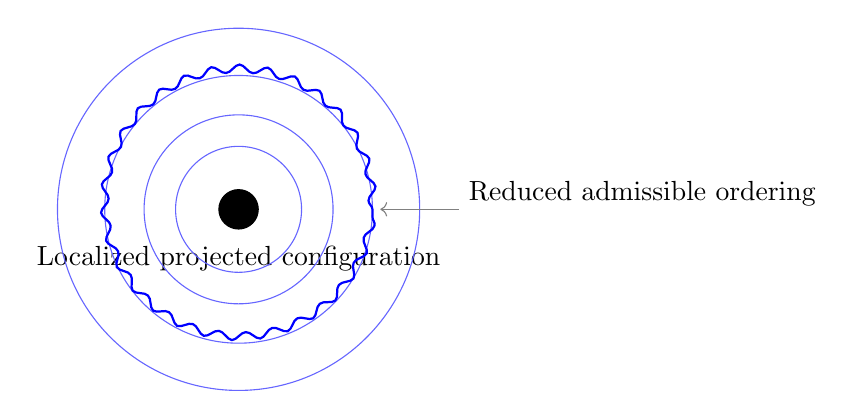
\begin{tikzpicture}[scale=1]

% Central mass
        \filldraw[black] (0,0) circle (0.25);
        \node[below] at (0,-0.35) {Localized projected configuration};

% Effective ordering contours
        \foreach \r in {0.8,1.2,1.7,2.3} {
          \draw[blue!60] (0,0) circle (\r);
        }

% Distortion
        \draw[blue, thick, decorate, decoration={snake, amplitude=0.5mm}]
        (0,0) circle (1.7);

% Arrows
        \draw[->, gray] (2.8,0) -- (1.8,0);
        \node[right] at (2.8,0.2) {Reduced admissible ordering};

      \end{tikzpicture}
      \caption
      {Emergence of Schwarzschild-like behavior in Cosmochrony.
      A localized projected configuration induces a spatially varying reduction of admissible relaxation ordering.
      In effective geometric descriptions, this manifests as differential proper-time
      accumulation and an emergent metric curvature analogous to gravitational time dilation.}
      \label{fig:chi_gravity}
    \end{figure}

  \input{07-gravity-as-a-collective-effect-of-particle-excitations/05-equivalence-principle}
  \input{07-gravity-as-a-collective-effect-of-particle-excitations/06-gravitational-waves}
  Before turning to strong-gravity regimes, it is useful to summarize the different
projective regimes discussed in this section.

\begin{figure}[h]
  \centering
  \begin{tabular}{c c c c c}
    \textbf{Projectable} &
    $\rightarrow$ &
    \textbf{Horizon} &
    $\rightarrow$ &
    \textbf{Non-projectable} \\[6pt]

    Gravitational &
    &
    Boundary of &
    &
    Deprojected \\
    Waves &
    &
    Projection &
    &
    Regime \\[6pt]

    Effective &
    &
    $\Pi$ non-injective &
    &
    No spacetime \\
    Modulations &
    &
    &
    &
    Representation
  \end{tabular}
  \caption{Conceptual regimes of projection in Cosmochrony.
  Gravitational waves correspond to fully projectable collective modulations of
  admissible descriptions, while black holes mark the boundary beyond which spacetime
  representations cease to be injective.
  Black hole evaporation reflects the gradual restoration of projectability,
    without any loss of information at the fundamental relational level,
    but only a loss and recovery of spacetime representability.}
  \label{fig:chi_projection_regimes}
\end{figure}

This schematic overview highlights how gravitational waves, horizons, and black hole
evaporation correspond to distinct regimes of projectability of the same underlying
relational structure.

\subsection{Strong Gravity and Black Holes}
  \label{subsec:strong-gravity-and-black-holes}

  In regions where the density of localized projected configurations becomes
  sufficiently high, admissible relaxation ordering becomes strongly constrained.
  In effective spacetime descriptions, this corresponds to a regime in which the local
  accumulation of effective time is strongly suppressed relative to distant observers,
  defining an effective horizon.

  Within Cosmochrony, such regions are interpreted as black holes.
  Rather than being characterized by a fundamental spacetime singularity, black holes
  correspond to domains where physical processes become asymptotically inaccessible
  from the exterior due to the loss of injectivity of spacetime projection.
  This naturally accounts for extreme time dilation effects without requiring divergent
  curvature invariants.

  These regions therefore mark not a terminal endpoint of physical description, but a
  transition toward a non-projectable regime of the underlying relational structure.

  \subsubsection*{Gravitational and Temporal Shadows}

    In the strong-gravity regime, the increasing concentration of localized projected
    configurations induces severe constraints on admissible ordering.
    As a result, the effective progression of time within the region slows
    asymptotically with respect to external descriptions.

    This behavior reproduces the phenomenon commonly referred to as a
    \emph{gravitational shadow}.
    In general relativity, such shadows arise from the absence of escaping null
    geodesics within a characteristic angular region.
    In Cosmochrony, an equivalent observational signature emerges because effective
    propagating descriptions, including radiation-like modes, no longer admit a faithful
    spacetime representation once projectability is lost.
    External observers therefore perceive a dark angular region corresponding to the
    projection of a non-projectable domain.

    Beyond this optical effect, the framework predicts a deeper phenomenon, which may be
    termed a \emph{temporal shadow}.
    As projectability is progressively lost, internal processes become indefinitely
    delayed in effective spacetime descriptions.
    From the external perspective, physical evolution appears frozen, providing a
    natural interpretation of horizon-induced time dilation.

    In this view, the observed gravitational shadow corresponds to the visible
    manifestation of an underlying temporal shadow.
    Both effects arise from the same loss of projective representability and do not
    require a fundamental spacetime singularity.

  \subsubsection*{Absence of Physical Singularities}

    In classical general relativity, black holes are associated with spacetime
    singularities characterized by divergent curvature and energy density.
    In Cosmochrony, such singularities are interpreted as artifacts of extending
    effective spacetime descriptions beyond their domain of validity.

    Because admissible ordering is bounded, configurations corresponding to infinite
    curvature or density cannot be physically realized.
    Apparent singularities therefore signal the breakdown of spacetime representability
    rather than genuine divergences of the underlying relational structure.

    \paragraph{Structural bound and notation.}
      To avoid confusion between fundamental and emergent levels, we distinguish the
      dimensionless structural bound $c_{\chi}$, defined at the level of the pre-geometric
      relational substrate, from its emergent spacetime manifestation $c$, interpreted as
      the maximal signal propagation speed.
      While $c$ may exhibit effective regime-dependent variations, the bound $c_{\chi}$ is
      invariant.

  \subsubsection*{Black Holes, Deprojection, and Vacuum Reprojection}
    \label{subsec:black-hole-deprojection-cycle}

    Within Cosmochrony, the absence of physical singularities does not imply that black
    holes are dynamically inert.
    Rather, they correspond to regimes in which the projection of relational information
    onto spacetime ceases to be injective.

    The emergence of an effective spacetime description relies on a projection map
    \[
      \Pi : \mathcal{C}_{\mathrm{rel}} \longrightarrow \mathcal{M},
    \]
    from the space of relational configurations to an effective spacetime manifold.
    In weak- and moderate-field regimes, this map is locally injective, ensuring a faithful
    geometric encoding.

    In strong-gravity regimes, this injectivity breaks down.
    Multiple inequivalent relational configurations correspond to the same effective
    spacetime event, signaling a loss of representability without any loss of information.
    We refer to this loss of injectivity as \emph{deprojection}.

    Deprojection does not correspond to transport across a spatial boundary nor to a
    temporal reversal.
    Instead, relational information ceases to be expressible in spatiotemporal form and
    remains encoded structurally.

    Importantly, deprojected information is not destroyed.
    Because the underlying relational configuration remains globally defined, information
    is in principle reprojectable once projectability is restored.
    Reprojection occurs discretely and manifests in effective spacetime descriptions as
    radiation-like excitations or particle--antiparticle pairs.

    The deprojection regime associated with black hole horizons does not imply the
    absence of dynamical processes.
    While smooth metric evolution ceases, the $\chi$ substrate remains structurally active.
    In particular, reprojection may occur intermittently when local configurations
    reach the threshold required for effective visibility.
    In the following section, this process is formalized through an explicit
    reprojection flux equation governing black hole evaporation.

    \paragraph{Information conservation and unitarity.}
      Deprojection does not correspond to information loss.
      It marks the loss of spacetime encoding, not the destruction of correlations.
      At the fundamental relational level, global information is preserved.
      Apparent non-unitarity arises only within projected spacetime descriptions and
      reflects their limited domain of applicability.

      This reprojection mechanism is analogous to vacuum fluctuations
      (Section~\ref{subsec:vacuum-fluctuations-and-the-casimir-effect}), where structural information is temporarily
      non-projectable before re-emerging as radiation.

  \subsection{Black Hole Evaporation and the Information Problem}
  \label{subsec:black-hole-evaporation-information}

  Within the Cosmochrony framework, black holes are not associated with physical
  singularities, but with regions where spacetime projection ceases to be injective.
  Such regions define domains of limited representability rather than physical interiors.

  \paragraph{Evaporation as a Projective Phenomenon.}
    Black hole evaporation is an effective process unfolding entirely within the
    projectable regime.
    It arises from the gradual restoration of projectability near the boundary separating
    projectable and non-projectable domains.

    As projectability is progressively recovered, localized projected configurations
    cease to be supported and are replaced by radiation-like effective descriptions.
    The evaporation process completes before any effective description would encounter a
    non-projectable singular regime.

  \paragraph{Resolution of the Information Paradox.}
    The apparent information loss identified by Hawking arises from treating spacetime as
    fundamental~\cite{Hawking1976}.
    In Cosmochrony, information is encoded in the global relational configuration
    independently of its spacetime projection.
    Evaporation therefore does not violate unitarity; it reflects a change in the domain
    of representability.

  \paragraph{Observational Implications.}
    To external observers, emitted radiation appears nearly thermal and weakly
    correlated with infalling states.
    This reflects the coarse-grained nature of spacetime projection rather than genuine
    information loss.
    The black hole information paradox is thus resolved by recognizing it as an artifact
    of extrapolating spacetime concepts beyond their domain of validity.

\subsubsection*{Horizon Reprojection Equation}
  \label{subsec:horizon-reprojection-equation}

  Within Cosmochrony, black hole evaporation is described as a reprojection process
  by which structural energy stored in the $\chi$ substrate is released into the projected
  spacetime in discrete units.

  The energy flux emerging from the horizon is defined as a sum over reprojection
  events associated with micro-configurations of the projection fiber:
  \[
    \Phi_\chi \equiv \frac{dE}{dt}
    = \sum_k \delta(t - t_k)\, \hbar_\chi\, \nu_k(L_{\mathrm{sol}}).
  \]

  Here, $\hbar_\chi$ denotes the fundamental quantum of reprojection, setting the
  minimal granularity of projected action.
  The quantities $\nu_k(L_{\mathrm{sol}})$ correspond to the resonance frequencies
  associated with the eigenmodes of the stability operator $L_{\mathrm{sol}}$ acting
  on the projection fiber $\Pi^{-1}(g_H)$ at the horizon, where $g_H$ denotes the
  effective near-horizon geometry.
  The times $t_k$ label the instants at which local $\chi$ configurations reach the
  projection threshold and become effectively visible in spacetime.

  Black hole evaporation thus proceeds as a sequence of discrete reprojection pulses,
  rather than as a continuous emission process.

\subsubsection*{Emergent Temperature and Relaxation Gradient}
  \label{subsec:emergent-temperature}

  The apparent Hawking temperature perceived by a distant observer emerges from the
  statistical distribution of reprojection events.
  It is determined by the gradient of effective $\chi$ relaxation normal to the horizon.

  This relation may be expressed as
  \[
    k_B T_\chi = \frac{\hbar_\chi c}{2\pi}\,
    \left| \nabla_{\perp} \chi_{\mathrm{eff}} \right|_H.
  \]

  For more massive black holes, the relaxation gradient is distributed over a larger
  horizon area, reducing the frequency of reprojection events.
  This directly explains the inverse mass–temperature relation without invoking
  vacuum particle creation or fundamental thermodynamic assumptions.

\subsubsection*{Information Conservation and Spectral Encoding}
  \label{subsec:information-conservation}

  In contrast with semiclassical descriptions, information is never destroyed in
  Cosmochrony.
  The projection operator $\Pi$ acts as a filter rather than as an irreversible map.

  During the deprojection phase, information is stored in the nonlinear degrees of
  freedom of the $\chi$ substrate, encoded within the projection fiber.
  During reprojection, the emitted radiation carries the precise spectral imprint of
  the eigenmodes governing the $\chi$ configuration.

  Each emitted quantum corresponds to a specific transition within the substrate,
  ensuring global unitarity.
  The apparent loss of information arises solely from restricting attention to the
  projected metric degrees of freedom.

\subsubsection*{Entropy as a Projection Saturation Limit}
  \label{subsubsec:entropy-projection-saturation}

  Within the Cosmochrony framework, the recovery of the Bekenstein--Hawking
  area law,
  \begin{equation}
    S = \frac{A}{4},
  \end{equation}
  does not rely on the introduction of a temperature or on thermodynamic
  postulates.
  Instead, black hole entropy is reinterpreted as a measure of the
  informational capacity of the projection map $\Pi$ at the horizon boundary.

  \paragraph{The Horizon as a De-projection Boundary}

    In the near-horizon regime, the $\chi$ substrate approaches a state of
    critical constraint in which the mapping
    \(
    \Pi : \chi \rightarrow g_{\mu\nu}
    \)
    ceases to be injective (see Section~7.7.3).
    The horizon is therefore redefined as the locus at which the local
    relaxation rate $N(r)$ vanishes, preventing further refinement of the
    projected metric degrees of freedom.

    At this boundary, distinct micro-configurations of the substrate are
    mapped onto the same effective horizon geometry $g_H$.
    Entropy is identified with the logarithmic measure of the fiber
    \(
    \Pi^{-1}(g_H),
    \)
    that is, the structural multiplicity of $\chi$ configurations that are no
    longer distinguishable at the metric level.
    Entropy thus quantifies hidden relational structure, rather than thermal
    ignorance.

    This situation is schematically illustrated in
    Figure~\ref{fig:projection-saturation-horizon}.

    \begin{figure}[htbp]
      \centering
      \resizebox{\linewidth}{!}{%
        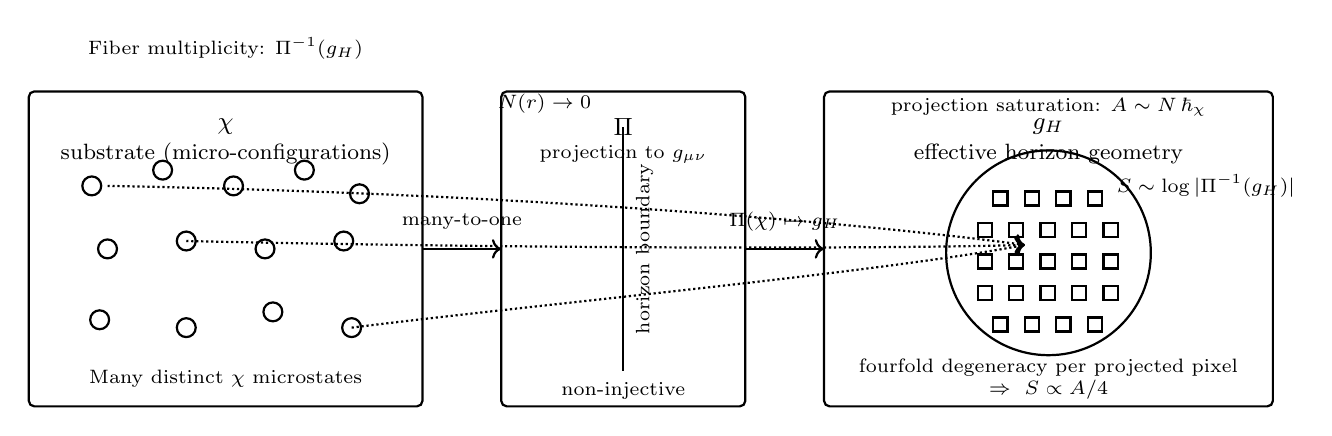
\begin{tikzpicture}[font=\small]

          % --- Geometry constants (implicit): boxes are placed in absolute coordinates ---
          % Left box: chi
          \draw[thick,rounded corners=2pt] (0,0) rectangle (5.0,4.0);
          \node at (2.5,3.55) {$\chi$};
          \node[font=\footnotesize] at (2.5,3.20) {substrate (micro-configurations)};

          % Middle box: projection / horizon boundary
          \draw[thick,rounded corners=2pt] (6.0,0) rectangle (9.1,4.0);
          \node at (7.55,3.55) {$\Pi$};
          \node[font=\scriptsize] at (7.55,3.20) {projection to $g_{\mu\nu}$};

          % Right box: g_H (keep minimal to avoid overlap)
          \draw[thick,rounded corners=2pt] (10.1,0) rectangle (15.8,4.0);
          \node at (12.95,3.55) {$g_H$};
          \node[font=\footnotesize] at (12.95,3.20) {effective horizon geometry};

          % --- Microstates (left box) ---
          \foreach \x/\y in {0.8/2.8,1.7/3.0,2.6/2.8,3.5/3.0,4.2/2.7,
          1.0/2.0,2.0/2.1,3.0/2.0,4.0/2.1,
          0.9/1.1,2.0/1.0,3.1/1.2,4.1/1.0}{
            \draw[thick] (\x,\y) circle (0.12);
          }
          \node[font=\scriptsize] at (2.5,0.35) {Many distinct $\chi$ microstates};

          % --- Arrow to middle box ---
          \draw[->,thick] (5.0,2.0) -- (6.0,2.0);
          \node[font=\scriptsize] at (5.5,2.35) {many-to-one};

          % --- Horizon boundary line inside middle box ---
          \draw[thick] (7.55,0.45) -- (7.55,3.55);
          \node[font=\scriptsize,rotate=90] at (7.82,2.0) {horizon boundary};
          \node[font=\scriptsize] at (6.55,3.85) {$N(r)\to 0$};
          \node[font=\scriptsize] at (7.55,0.20) {non-injective};

          % --- Arrow to right box ---
          \draw[->,thick] (9.1,2.0) -- (10.1,2.0);
          \node[font=\scriptsize] at (9.6,2.35) {$\Pi(\chi)\mapsto g_H$};

          % --- Horizon disk + pixels (right box) ---
          \draw[thick] (12.95,1.95) circle (1.30);
          \node[font=\scriptsize] at (12.95,3.80) {projection saturation: $A \sim N\,\hbar_\chi$};

          % pixels inside the disk (all are safely inside)
          \foreach \x/\y in {12.25/2.55,12.65/2.55,13.05/2.55,13.45/2.55,
          12.05/2.15,12.45/2.15,12.85/2.15,13.25/2.15,13.65/2.15,
          12.05/1.75,12.45/1.75,12.85/1.75,13.25/1.75,13.65/1.75,
          12.05/1.35,12.45/1.35,12.85/1.35,13.25/1.35,13.65/1.35,
          12.25/0.95,12.65/0.95,13.05/0.95,13.45/0.95}{
            \draw[thick] (\x,\y) rectangle ++(0.18,0.18);
          }

          % --- Dotted arrows: selected microstates collapse to same horizon pixel ---
          \draw[->,thick,densely dotted] (1.0,2.8) .. controls (6.5,2.7) and (10.8,2.3) .. (12.65,2.05);
          \draw[->,thick,densely dotted] (2.0,2.1) .. controls (6.5,2.0) and (10.8,2.0) .. (12.65,2.05);
          \draw[->,thick,densely dotted] (4.1,1.0) .. controls (6.5,1.3) and (10.8,1.7) .. (12.65,2.05);

          % --- External annotations (kept outside boxes to avoid overlap) ---
          \node[font=\scriptsize,align=left] at (2.5,4.55) {Fiber multiplicity: $\Pi^{-1}(g_H)$};
          \node[font=\scriptsize,align=left] at (14.95,2.80) {$S \sim \log |\Pi^{-1}(g_H)|$};
          \node[font=\scriptsize,align=center] at (12.95,0.35)
            {fourfold degeneracy per projected pixel\\$\Rightarrow\ S \propto A/4$};

        \end{tikzpicture}%
      } % resizebox

      \caption{
        Saturation of the projection map at the horizon.
        Near the boundary where $N(r)\to 0$, the projection $\Pi$ becomes non-injective:
        multiple micro-configurations of the $\chi$ substrate collapse onto the same
        effective horizon geometry $g_H$.
        Entropy measures the structural multiplicity of the fiber $\Pi^{-1}(g_H)$ and the
        saturation of projected metric ``pixels'' of area $\sim \hbar_\chi$.
      }
      \label{fig:projection-saturation-horizon}
    \end{figure}

  \paragraph{Geometric Origin of the \texorpdfstring{$1/4$}{1/4} Factor}

    The numerical factor $1/4$ arises as a structural ratio between the
    internal degrees of freedom of the $\chi$ substrate and their maximal
    holographic projection onto a two-dimensional boundary.

    Let $\hbar_\chi$ denote the elementary quantum of reprojection.
    The horizon area $A$ is saturated by a finite number $N$ of effective
    pixels of area $\sim \hbar_\chi$.
    Within the Cosmochrony framework, each such projected pixel corresponds to
    a fourfold degeneracy in the stability spectrum of $\chi$, linked to the
    intrinsic $4\pi$ periodicity of $\chi$ excitations discussed in
    Section~5.2.

    The area law
    \(
    S = A/4
    \)
    is therefore the macroscopic signature of this quadrature constraint:
    it represents the maximal density of independent structural degrees of
    freedom that can be projected before the non-injectivity of $\Pi$ induces
    a complete loss of local metric resolution.

  \paragraph{Unitary Reprojection and Information Conservation}

    Black hole evaporation is reformulated as a discrete reprojection
    process.
    As the $\chi$ substrate locally relaxes at the horizon boundary, it emits
    quanta of action $\hbar_\chi$ carrying the spectral imprint of the fiber
    $\Pi^{-1}(g_H)$.

    Because this process is governed by the deterministic---though
    nonlinear---relaxation dynamics of $\chi$, information is never destroyed
    nor trapped in a singularity.
    Instead, it is transferred from a purely structural encoding within the
    fiber back into observable spacetime degrees of freedom.
    Unitarity is preserved at the level of the $\chi$ substrate, even though
    the effective spacetime description may exhibit apparent non-unitarity.

  \paragraph*{Conclusion}

    In Cosmochrony, black hole entropy is not a measure of ignorance but a
    measure of projection saturation.
    It quantifies the threshold at which the complexity of the $\chi$
    substrate exceeds the transmittance capacity of the effective metric
    projection.
    This explains why entropy scales with area---the projection surface---and
    not with volume, which characterizes the inaccessible internal fiber.

  \input
  {07-gravity-as-a-collective-effect-of-particle-excitations/09-unified-origin-of-gravitational-and-electromagnetic-effects}
  \subsection{Summary}
  \label{subsec:summary6}

  Within the Cosmochrony framework, gravity does not arise as a fundamental interaction
  or as an independent geometric degree of freedom.
  It emerges at the level of effective descriptions as a macroscopic consequence of
  localized projected configurations collectively constraining admissible relaxation
  ordering.

  Classical gravitational phenomena—including gravitational time dilation, effective
  spacetime curvature, gravitational waves, and black holes—are recovered as distinct
  descriptive regimes of this collective constraint.
  They reflect variations in the projectability and correlation structure of admissible
  descriptions, rather than the dynamics of a fundamental spacetime or gravitational
  field.

  In this perspective, gravitation appears as an emergent, operational phenomenon,
  summarizing how localized projected configurations collectively limit admissible
  ordering and correlation across extended regions, without introducing gravity as a
  primitive force or fundamental geometric entity.



  \section{Quantum Correlations and Entanglement}
    \label{sec:quantum-correlations-and-entanglement}
    \input{07-quantum-correlations-and-entanglement}

  \section{Relation to Quantum Formalism}
    \label{sec:relation-to-quantum-formalism}
    This section does not assign fundamental ontological status to the quantum wavefunction
or to Hilbert space structures.
Instead, it shows how the formal apparatus of quantum mechanics can be understood
as an effective framework emerging from the dynamics of localized and weakly interacting
$\chi$-field excitations described in the preceding sections.

\subsection{Status of the Wavefunction}\label{subsec:status-of-the-wavefunction}

  In standard quantum mechanics, the wavefunction $\psi$
  is a complex-valued object defined on configuration space, whose ontological status remains debated.
  Operationally, $|\psi|^2$ encodes measurement probabilities via the Born rule, while $\psi$
  itself does not correspond directly to a physical field in spacetime.

  In cosmochrony, the $\chi$ field is not identified with the quantum wavefunction.
  Instead, $\chi$
  constitutes a real geometric substratum defined on spacetime, from which effective quantum wavefunctions
  emerge as coarse-grained descriptions of localized excitations.
  The quantum wavefunction is thus interpreted as a derived object encoding the statistical behavior of $\chi$
  -mediated structures rather than as a fundamental entity.

  As an example, the hydrogen atom's wavefunction $\psi_{nlm}(r, \theta, \phi)$
  corresponds to a stable solitonic configuration of $\chi$ with radial nodes $n$, angular momentum $l$,
  and magnetic quantum number $m$. The probability density $|\psi|^2$ reflects the spatial distribution of
  $\chi$-curvature, while energy quantization $E_n \propto -1/n^2$
  arises from the discrete topological winding numbers permitted by the boundary conditions at $r \to 0$ and
  $r \to \infty$.

\subsection{Emergence of Hilbert Space Structure}\label{subsec:emergence-of-hilbert-space-structure}

  The Hilbert space formalism of quantum mechanics provides a linear structure supporting superposition,
  interference, and unitary evolution.
  Within cosmochrony, this structure arises as an effective description of weakly interacting excitations of the
  $\chi$ field.

  Linear superposition reflects the approximate independence of small-amplitude perturbations propagating on a
  slowly varying $\chi$ background.
  The complex phase of the wavefunction encodes relative geometric shifts within the underlying $\chi$
  oscillations rather than representing an intrinsic complex field.

\subsection{Emergence of the Schrödinger Equation from $\chi$ Fluctuations}
  \label{sec:schrodinger_emergence}

  In Cosmochrony, quantum behavior is not postulated but emerges as an effective,
  long-wavelength description of small fluctuations of the fundamental $\chi$ field
  around stable solitonic configurations. In this section, we provide an explicit and
  standard derivation of the Schr\"odinger equation as the non-relativistic limit of such
  fluctuations, making all approximations transparent.

  \subsubsection{Non-relativistic limit: Klein--Gordon $\rightarrow$ Schr\"odinger}
    \label{sec:KGtoSch}

    Consider a localized, massive excitation of the Cosmochrony field around a quasi-stationary soliton
    background,
    \begin{equation}
      \chi(x,t)=\chi_{\mathrm{sol}}(x)+\delta\chi(x,t),
    \end{equation}
    and assume that, to leading order in small fluctuations, $\delta\chi$ obeys an effective
    Klein--Gordon equation with a mass scale $m$ set by the soliton's rest-energy:
    \begin{equation}
      \left(\frac{1}{c^{2}}\partial_{t}^{2}-\nabla^{2}+\frac{m^{2}c^{2}}{\hbar^{2}}\right)\delta\chi=0.
      \label{eq:KG_eff}
    \end{equation}

    In the non-relativistic regime, the field oscillates rapidly at the rest-energy frequency
    $\omega_{0}=mc^{2}/\hbar$, while its envelope varies slowly. We therefore use the standard ansatz
    \begin{equation}
      \delta\chi(x,t)=\psi(x,t)\,e^{-i\omega_{0}t},
      \qquad
      \left|\partial_t\psi\right|\ll\omega_{0}|\psi|.
      \label{eq:NR_ansatz}
    \end{equation}
    Compute derivatives:
    \begin{align}
      \partial_t\delta\chi &= e^{-i\omega_0 t}\left(\partial_t\psi-i\omega_0\psi\right),\\
      \partial_t^2\delta\chi &= e^{-i\omega_0 t}
      \left(\partial_t^2\psi-2i\omega_0\partial_t\psi-\omega_0^2\psi\right),
    \end{align}
    and substitute into Eq.~\eqref{eq:KG_eff}. Using $\omega_0=mc^2/\hbar$ cancels the large rest-mass
    terms ($-\omega_0^2/c^2$ against $+m^2c^2/\hbar^2$), yielding
    \begin{equation}
      \frac{1}{c^2}\partial_t^2\psi-\frac{2i\omega_0}{c^2}\partial_t\psi-\nabla^2\psi=0.
      \label{eq:KG_env}
    \end{equation}
    Under the slow-envelope condition, $\left|\partial_t^2\psi\right|\ll\omega_0\left|\partial_t\psi\right|$
    (neglecting terms of order $v^4/c^4$), Eq.~\eqref{eq:KG_env} reduces to
    \begin{equation}
      -\frac{2i\omega_0}{c^2}\partial_t\psi-\nabla^2\psi=0
      \quad\Longrightarrow\quad
      i\hbar\,\partial_t\psi=-\frac{\hbar^2}{2m}\nabla^2\psi.
      \label{eq:Sch_free}
    \end{equation}

    A weak interaction with the surrounding $\chi$ background (or other solitons) can be encoded at the
    envelope level by an effective potential $V(x)$, giving the standard Schr\"odinger form
    \begin{equation}
      i\hbar\,\partial_t\psi=\left[-\frac{\hbar^2}{2m}\nabla^2+V(x)\right]\psi.
      \label{eq:Sch_V}
    \end{equation}

    \paragraph{Cosmochrony-specific content.}
      Equations~\eqref{eq:Sch_free}--\eqref{eq:Sch_V} establish the rigorous non-relativistic limit of a
      relativistic scalar excitation. In Cosmochrony, the program is to derive (i) the effective mass
      $m$ from soliton energetics and (ii) the form of $V(x)$ from interaction-induced deformations of
      $\chi_{\mathrm{sol}}(x)$.

  \subsubsection{Interpretation}

    In this framework, the complex wavefunction $\psi$ does not represent a fundamental
    quantum object but an effective description of coherent $\chi$-field fluctuations
    around a solitonic particle state. The Schr\"odinger equation thus appears as the
    universal non-relativistic limit of localized $\chi$ excitations, rather than as a
    fundamental postulate.

    The Cosmochrony program is to relate the effective mass and interaction potential
    entering the Schr\"odinger dynamics to soliton energetics and interaction-induced
    deformations of the $\chi$ background. A detailed derivation of these quantities from
    the full $\chi$ action is left for future work.

\subsection{Origin of Quantization}\label{subsec:origin-of-quantization}

  Quantization in standard quantum theory is postulated through canonical commutation relations or path-integral
  prescriptions.

  In cosmochrony, discrete energy exchanges arise from topological constraints on stable excitations of the $\chi$
  field.
  Only certain winding numbers, knot structures, or resonance conditions are dynamically stable, leading to
  effectively quantized energy levels.
  The relation $E = h \nu$
  emerges as a geometric proportionality between oscillation frequency and curvature energy stored in localized
  $\chi$ configurations.

\subsection{Measurement and the Born Rule}\label{subsec:measurement-and-the-born-rule}

  The measurement postulate remains one of the most conceptually opaque elements of quantum mechanics.
  In cosmochrony, measurement corresponds to a local irreversible interaction between a structured excitation and
  stochastic fluctuations of the $\chi$ field.

  Detection events occur when interference between the excitation and ambient $\chi$
  fluctuations produces a stable localized crest.
  The Born rule arises statistically from the distribution of these fluctuations, with $|\psi|^2$
  representing the density of favorable geometric configurations rather than a fundamental probability axiom.

  During a measurement, the detector's macroscopic degrees of freedom impose boundary conditions that select a
  specific topological sector of the $\chi$
  -field. For example, a photon detector absorbs energy by fixing a localized crest in $\chi$
  , effectively ``cutting'' the extended wave configuration and collapsing it to a particle-like excitation. The
  Born rule $P \propto |\psi|^2$ then follows from the statistical distribution of $\chi$
  -fluctuations that satisfy the detector's constraints, without requiring an intrinsic probabilistic postulate.

\subsection{Entanglement and Nonlocal Correlations}\label{subsec:entanglement-and-nonlocal-correlations}

  Quantum entanglement is traditionally described as nonlocal correlation between subsystems whose joint
  wavefunction cannot be factorized.

  In cosmochrony, entanglement corresponds to persistent geometric connectedness within a single extended $\chi$
  configuration.
  Separated particles remain correlated because they are manifestations of the same underlying wave segment.
  Decoherence corresponds to the progressive tearing or dispersion of this shared geometric structure due to
  environmental interactions.

  This interpretation preserves the empirical predictions of quantum mechanics while avoiding superluminal
  signaling, as no information propagates faster than the local relaxation rate of $\chi$.

\subsection{Spin and Statistics}\label{subsec:spin-and-statistics}

  Spin is treated in quantum mechanics as an intrinsic degree of freedom associated with representations of the
  rotation group.
  The necessity of $4\pi$
  rotations for fermions is usually accepted as a mathematical fact without deeper geometric explanation.

  Within cosmochrony, half-integer spin emerges from topological twists of $\chi$ excitations.
  Fermionic states correspond to M\"obius-like configurations requiring $4\pi$
  rotations to return to identity, while bosonic states correspond to untwisted or integer-winding structures.
  The spin-statistics connection follows naturally from the topological stability of these configurations.

  See an illustrated example in ~\ref{subsec:4pi_soliton}.

\subsection{Scope and Limitations}\label{subsec:scope-and-limitations}

  Cosmochrony does not aim to replace the quantum formalism.
  All standard computational tools of quantum mechanics remain valid within their domain of applicability.

  The contribution of cosmochrony is interpretative and unificatory: it proposes a geometric origin for quantum
  behavior, measurement statistics, and nonlocal correlations, without modifying experimentally tested predictions.
  Further work is required to formalize the precise mapping between $\chi$
  dynamics and operator-based quantum theory.


  \section{Cosmological Implications}
    \label{sec:cosmology}
    \subsection{Cosmic Expansion as $\chi$ Relaxation}
  \label{subsec:cosmic-expansion-as-$chi$-relaxation}

  In cosmochrony, cosmic expansion is not driven by an initial impulse or by a cosmological constant.
  Instead, it results from the monotonic relaxation of the $\chi$ field toward larger characteristic wavelengths.

  As $\chi$ increases uniformly, spatial separations between comoving points grow proportionally.
  The recession velocity between distant objects thus arises as a cumulative effect of local $\chi$
  relaxation rather than as motion through space.

  \begin{figure}[h]
    \centering
    \begin{tikzpicture}[scale=1]

% Axes
      \draw[->] (0,0) -- (6,0) node[right]{Cosmic time};
      \draw[->] (0,0) -- (0,4) node[above]{Scale / Wavelength};

% LambdaCDM
      \draw[thick, gray, dashed]
      plot[smooth] coordinates {(0.5,0.7) (2,1.3) (4,2.5) (5.5,3.7)};
      \node[gray] at (4.5,3.2) {$\Lambda$CDM};

% Chi relaxation
      \draw[thick, blue]
      plot[smooth] coordinates {(0.5,0.8) (2,1.4) (4,2.2) (5.5,2.9)};
      \node[blue] at (4.7,2.5) {$\chi(t)$};

    \end{tikzpicture}
    \caption{Comparison between standard $\Lambda$CDM cosmological expansion and Cosmochrony. In the latter,
      the observed Hubble law emerges from the monotonic relaxation of the fundamental field $\chi$,
      without invoking dark energy.}
    \label{fig:cosmo_comparison}
  \end{figure}

  Primordial fluctuations in $\chi$ at the recombination epoch ($z \sim 1100$
  ) are imprinted as temperature anisotropies in the CMB. The near scale-invariance of these fluctuations
  reflects the universal relaxation dynamics of $\chi$
  , while their acoustic peaks arise from oscillatory coupling between $\chi$
  and matter excitations. Unlike inflationary models, no superluminal stretching is required: correlations
  extend across the observable universe because they originate from a single connected $\chi$
  -field configuration prior to relaxation.

\subsection{Emergent Hubble Law}
  \label{subsec:emergent-hubble-law}

  Let $\chi(t)$ denote the spatially averaged value of the field.
  The effective scale factor $a(t)$ scales proportionally to $\chi(t)$:
  \begin{equation}
    a(t) \propto \chi(t).
  \end{equation}

  The Hubble parameter follows directly:
  \begin{equation}
    H(t) = \frac{\dot{a}}{a} = \frac{\dot{\chi}}{\chi}.
  \end{equation}

  Assuming maximal relaxation speed $\dot{\chi} = c$, the present value of the Hubble constant becomes
  \begin{equation}
    H_0 \approx \frac{c}{\chi(t_0)},
  \end{equation}
  providing a natural scale for cosmic expansion without introducing dark energy.

\subsection{Cosmic Acceleration Without Dark Energy}
  \label{subsec:cosmic-acceleration-without-dark-energy}

  Because $\chi$ relaxation accumulates over time, recession velocities increase with distance.
  This leads to an apparent acceleration when interpreted through conventional cosmological models.

  In cosmochrony, this effect does not reflect a change in the expansion rate but the cumulative nature of $\chi$
  growth.
  Thus, accelerated expansion emerges without requiring a cosmological constant or exotic energy components.

\subsection{Cosmic Microwave Background}
  \label{subsec:cosmic-microwave-background}

  In this model, the Cosmic Microwave Background (CMB) reflects frozen fluctuations of the $\chi$
  field at the epoch when matter-radiation interactions decoupled.

  Primordial variations in $\chi$
  phase and amplitude imprint temperature anisotropies that persist as large-scale correlations.

  These fluctuations originate from stochastic variations in local $\chi$
  relaxation prior to large-scale structure formation.
  Their near scale invariance reflects the universal relaxation dynamics of the field.

  Unlike inflationary scenarios, no superluminal expansion is required to explain horizon-scale coherence:
  correlations originate from the pre-relaxation continuity of $\chi$.

  Further details on how $\chi$-field fluctuations reproduce the observed CMB anisotropies---including solutions to the
  horizon and flatness problems without inflation, as well as predicted deviations at large angular scales---are
  provided in Appendices~\ref{subsec:chi_cmb_spectrum} and~\ref{subsec:cosmochrony_horizon_flatness}.

\subsection{Hubble Tension}
  \label{subsec:hubble-tension}

  Measurements of the Hubble constant derived from early-universe observables~\cite{Planck2020,Riess2019}
  , such as the CMB, probe smaller values of $\chi$.
  In contrast, late-time measurements using local distance ladders correspond to larger accumulated $\chi$ values.

  This difference naturally produces a tension between inferred values of $H_0$
  without invoking systematic errors or new particles.

  The CMB anisotropy spectrum in the $\chi$-framework differs from inflationary predictions in the low-$\ell$
  regime, where the absence of a primordial inflationary phase would suppress large-angle correlations. This
  could be tested by future high-precision CMB experiments like CMB-S4 or LiteBIRD\@.

  The predicted decrease of $H_0$
  with cosmic time provides a natural explanation for the current Hubble tension.
  Early-universe probes (e.g., CMB-based measurements yielding $H_0 \approx 67 \, \text{km/s/Mpc}$) sample smaller $\chi$
  values than late-time distance ladder methods ($H_0 \approx 74 \, \text{km/s/Mpc}$), consistent with the observed $\sim 4.4\sigma$
  discrepancy.
  Although this numerical agreement should not be interpreted as a precision prediction, it is an indication that the
  framework naturally selects the observed cosmological scale. Future measurements of $H(z)$ across redshift ranges may
  distinguish between this geometric interpretation and dark energy models.

  This mechanism suggests that the ``tension'' is not a failure of the standard cosmological model but a
  manifestation of the non-linear coupling between matter density and the field’s relaxation rate.
  A formal derivation of this local correction, yielding an $8.4\%$ increase in $H_0$ within the KBC void, is detailed
  in Appendix~\ref{appendix:hubble_tension}.
\section{Cosmological Implications}
\label{sec:cosmology}

\subsection{Entropy and the Arrow of Time}
  \label{subsec:entropy-and-the-arrow-of-time}

  The monotonic increase of $\chi$ defines a preferred temporal direction that is fundamental within the
  Cosmochrony framework.
  This direction is not introduced through thermodynamic or statistical arguments but follows directly
  from the irreversible relaxation of the underlying field.

  As $\chi$ grows, localized excitations become increasingly separated and their configurations progressively
  lose the ability to reconcentrate relaxation potential.
  This leads to an effective irreversibility at the level of composite systems, even though the underlying
  dynamics of $\chi$ remains deterministic.

  Entropy increase is therefore interpreted as an emergent, coarse-grained description of this relaxation
  process, rather than as a fundamental driver of temporal ordering.
  In this view, thermodynamic entropy does not define the arrow of time but reflects it: the macroscopic
  growth of entropy mirrors the monotonic expenditure of the relaxation capacity of the $\chi$ field.

\subsection{Summary}
  \label{subsec:summary4}

  Cosmological expansion, apparent acceleration, the Hubble law, the CMB, and the arrow of time all emerge from the
  universal relaxation of the $\chi$ field.
  Cosmochrony reproduces key cosmological observations without introducing dark energy or modifying general
  relativity at large scales.


  \section{Radiation and Quantization}
    \label{sec:radiation-and-quantization}
    \section{Radiation and Quantization}
  \label{sec:radiation-and-quantization}

  \subsection{Radiation as $\chi$--Matter Interaction}
  \label{subsec:radiation-as-chimatter-interaction}

  Within the Cosmochrony framework, radiation does not correspond to the emission or
  propagation of fundamental particle entities.
  It arises as an effective phenomenon associated with the reconfiguration of
  localized matter descriptions and their relational coupling to the surrounding
  $\chi$ substrate.

  When a localized, relaxation-resistant configuration undergoes a transition toward
  a less constrained state, part of the relational structure that sustained its
  previous persistence becomes incompatible with continued localization.
  This excess relational content ceases to admit a particle-like projected
  description and instead becomes expressible only through delocalized projected
  modes.

  In effective spacetime descriptions, this redistribution appears as radiative
  emission.
  Radiation thus represents the loss of localized projectability and the transfer of
  descriptive weight from particle-like configurations to propagating field-like
  descriptions, without invoking the transport of discrete objects or underlying
  stochastic processes.

  From this perspective, radiative phenomena reflect a change in the organization and
  projectability of relational structure within $\chi$, rather than the emission of
  pre-existing quanta or the manifestation of fundamental fluctuations.

  \subsection{Emergence of Photons}
  \label{subsec:emergence-of-photons}

  In the Cosmochrony framework, photons are not fundamental entities, nor are they
  identified with propagating disturbances of the $\chi$ substrate.
  They arise as effective descriptions associated with transitions between localized
  and delocalized regimes of projectability.

  Prior to emission or detection, no photon exists as an independent object.
  What exists is a reconfiguration of relational structure within $\chi$ that ceases
  to admit a localized particle-like projection and becomes expressible only through
  extended, delocalized effective modes.

  In effective spacetime descriptions, these delocalized regimes are represented as
  electromagnetic waves.
  However, this wave character does not correspond to a physical oscillation of $\chi$,
  but to a continuous descriptive projection of relational structure compatible with
  field-like representation.

  Photon-like events emerge only at interaction.
  When a delocalized projective mode becomes locally constrained by interaction with a
  localized excitation (such as an atom or detector), the projection collapses into a
  discrete transfer of relaxation capacity.
  Quantization is therefore not a property of propagation, but of interaction and
  local reprojection.

  In this sense, wave--particle duality reflects a duality of description rather than a
  duality of underlying ontology.
  Interference phenomena, such as those observed in double-slit experiments, arise from
  the coherence of delocalized projective modes, while individual detection events
  correspond to localized reprojections.
  No fundamental wavefunction collapse or stochastic emission process is required.

  \subsection{Geometric Origin of $E = h\nu$}
  \label{subsec:energy-frequency-radiation}

  This section develops, in the context of radiative processes, the energy--frequency
  relation introduced earlier in
  Section~\ref{subsec:energy-frequency-solitons}, while remaining fully consistent with
  the non-propagative and pre-geometric nature of the $\chi$ substrate.

  In Cosmochrony, radiative events do not correspond to the emission of physical waves
  or disturbances propagating within the $\chi$ field.
  Instead, they correspond to transitions between localized and delocalized regimes of
  effective projectability.
  During such events, a portion of the relaxation potential stored in a localized
  matter excitation becomes expressible only through an extended, non-localized
  projective description.

  Within effective spacetime representations, these delocalized regimes are described
  using oscillatory field modes characterized by a frequency $\nu$.
  This frequency does not represent a fundamental oscillation of $\chi$, but a
  parameter labeling the internal structural periodicity of the effective description
  required to represent the released relaxation potential.

  The Planck relation
  \begin{equation}
    E = h \nu
  \end{equation}
  thus acquires a geometric interpretation.
  The energy $E$ measures the amount of relaxation potential redistributed during a
  reprojection event, while the frequency $\nu$ characterizes the minimal temporal
  resolution required for a coherent effective description of this redistribution.

  The proportionality constant $h$ does not encode a fundamental quantum postulate.
  As derived in Section~\ref{subsec:renormalization-hbar}, $h$ is the \textbf{effective projection}
  of the fundamental substrate invariant $\hbar_\chi \equiv c^3 / (K_{0,\text{bare}} \chi_{c,\text{bare}})$.
  It acts as a universal conversion factor linking the structural relaxation capacity of
  the substrate to the temporal resolution of the projective description.

  This interpretation explains why energy transfer in radiative processes scales
  linearly with frequency across a wide range of phenomena.
  In the photoelectric effect, the threshold frequency $\nu_0$ corresponds to the
  minimal projective resolution required to destabilize a bound electronic soliton.
  Above this threshold, the linear dependence on $\nu$ reflects the additional
  relaxation capacity made accessible through the reprojection process.

  In this sense, quantization of radiative energy does not arise from discretized
  propagation, but from the discrete nature of local \textbf{reprojection events},
  which impose a minimal unit of effective relaxation transfer determined by the
  spectral graininess ($\hbar_\chi$) of the underlying $\chi$ substrate.

  \subsection{Vacuum Fluctuations and the Casimir Effect}
  \label{subsec:vacuum-fluctuations-and-the-casimir-effect}

  In the Cosmochrony framework, vacuum fluctuations do not correspond to physical
  oscillations of a background field nor to spontaneous particle--antiparticle
  creation.
  Instead, they reflect the intrinsic structural indeterminacy of the $\chi$ substrate
  in regimes where no stable localized excitations are present.

  In the absence of matter-induced constraints, the relaxation of $\chi$ admits a wide
  range of locally compatible projective descriptions.
  These fluctuations are not dynamical events occurring \emph{in} spacetime, but
  expressions of the fact that the underlying relational structure of $\chi$ does not
  select a unique effective configuration when projected.
  They therefore represent variability of effective descriptions rather than physical
  energy stored in the vacuum.

  When material boundaries are introduced, they impose structural constraints on the
  local projectability of $\chi$.
  Certain effective descriptions become incompatible with the imposed relational
  conditions, reducing the set of admissible projective configurations between the
  boundaries compared to the exterior region.

  The Casimir effect arises from this asymmetry.
  It reflects a difference in the density of admissible effective reprojections
  compatible with the boundary conditions, which manifests in spacetime descriptions
  as a pressure acting on the confining surfaces.
  No fundamental vacuum energy density or propagating vacuum modes are required.

  In this sense, the Casimir effect probes the relational relaxation capacity of the
  $\chi$ substrate under imposed constraints, rather than revealing the presence of a
  physical zero-point energy filling space.

  \subsection{Weakly Interacting Radiation}
  \label{subsec:weakly-interacting-radiation}

  In the Cosmochrony framework, weakly interacting radiation does not correspond to
  fundamentally different particle species, but to $\chi$ disturbances whose
  structural contrast and curvature are insufficient to efficiently induce
  localized reprojection when encountering matter.

  Low-frequency electromagnetic disturbances or weakly coupled excitation patterns
  are characterized by smooth, slowly varying relational structure.
  As a result, their interaction with localized $\chi$ configurations is rare:
  the probability that such disturbances trigger a stable localized energy transfer
  upon interaction is strongly suppressed.

  This explains the effective transparency of vacuum to most radiation.
  Propagation corresponds to the persistence of a coherent $\chi$ disturbance across
  extended regions, while detection events occur only when local structural conditions
  allow reprojection into a localized excitation.

  In this sense, small interaction cross sections do not reflect the weakness of a
  fundamental force, but the low likelihood that a given disturbance of $\chi$
  satisfies the geometric and topological conditions required for localized
  reprojection.

  \subsection{Summary}
  \label{subsec:summary8}

  Within the Cosmochrony framework, entanglement does not arise as a fundamental
  property of an underlying physical field.
  It emerges at the level of effective descriptions as the persistence of
  non-factorizable admissible projected configurations across interactions and
  spacetime separation.

  Quantum correlations therefore arise without superluminal signaling, fundamental
  wavefunction collapse, or violations of relativistic causality.
  They reflect the global consistency constraints of admissible projected
  descriptions, rather than any dynamical nonlocal influence.

  Within this perspective, quantum phenomena arise from the tension between global
  descriptive coherence and local projectability.
  The standard quantum-mechanical formalism emerges as an effective statistical
  framework encoding the probabilities of locally accessible reprojections once
  non-factorizable descriptions can no longer be jointly represented.

  In this sense, quantum mechanics is not a fundamental ontology but a consistent
  effective theory describing the limits of factorization and projectability of
  physical descriptions within spacetime.



  \section{Testable Predictions and Observational Signatures}
    \label{sec:testable-predictions-and-observational-signatures}
    \input{11-predictions}

  \section{Discussion and Comparison with Existing Frameworks}
  \label{sec:discussion-and-comparison-with-existing-frameworks}

  The Cosmochrony framework proposes a minimal pre-geometric substrate, described by
  a single scalar quantity $\chi$, whose irreversible relaxation underlies both
  microscopic and cosmological phenomena.
  Spacetime geometry, gravitational dynamics, and quantum behavior arise only as
  effective descriptions of this underlying relaxation process.

  In this section, we discuss how this approach relates to established theoretical
  frameworks, highlight its conceptual implications, and identify open challenges.
  Particular emphasis is placed on clarifying points of contact and distinction with
  general relativity, quantum mechanics, and standard cosmological models, as well as
  on assessing the ontological and methodological economy of the framework.

  The goal is not to claim empirical superiority over existing theories, but to
  clarify the conceptual role of Cosmochrony as a deeper explanatory layer from which
  standard frameworks emerge in appropriate regimes.

  \subsection{Relation to General Relativity}
  \label{subsec:relation-to-general-relativity}

  General Relativity (GR) describes gravitation as the curvature of spacetime induced
  by energy--momentum.
  In Cosmochrony, no \emph{a priori} metric dynamics is postulated at the fundamental
  level.
  Instead, an effective spacetime geometry emerges as a descriptive framework from
  variations in the local relaxation dynamics of the $\chi$ field.

  Matter configurations, modeled as stable or metastable topological excitations of
  $\chi$, locally constrain the relaxation of the field.
  This leads to differential rates of effective proper-time evolution between
  neighboring regions.
  When expressed in geometric terms, these differences can be reinterpreted as an
  effective deformation of the spacetime metric.

  In the weak-field regime, this mechanism reproduces Newtonian gravity, while in the
  strong-field limit it yields Schwarzschild-like solutions in effective geometric
  descriptions.
  The resulting phenomenology is therefore consistent with the empirical successes
  of GR across its tested domain.

  From this perspective, gravitation is not introduced as a fundamental interaction,
  but emerges as a macroscopic manifestation of inhomogeneous $\chi$ relaxation.
  General Relativity is recovered as the appropriate effective theory describing
  this regime, rather than being supplanted or modified at the level of observable
  predictions.

  \subsection{Relation to Quantum Formalism}
  \label{subsec:relation-to-quantum-formalism}

  Quantum mechanics and quantum field theory (QFT) introduce probabilistic
  wavefunctions, operators, and quantization rules as foundational postulates~\cite{PeskinSchroeder1995QFT}.
  In contrast, Cosmochrony does not treat quantization or wave dynamics as fundamental.
  Instead, it describes a continuous pre-geometric relational substrate whose
  projected and thresholded effective descriptions give rise to the formal apparatus of quantum theory.

  Within this framework, particles correspond to localized, topologically stable configurations of the $\chi$ substrate.
  Discrete observables arise not from intrinsic microscopic discreteness, but from
  boundary conditions, topological constraints, and interaction-induced
  reprojection, which select a finite set of stable effective configurations.

  The Planck relation $E = h\nu$ is interpreted geometrically as a correspondence
  between the amount of relaxation potential redistributed during an interaction
  and the minimal projective resolution required for a coherent effective spacetime description.
  The parameter $\nu$ does not represent a fundamental oscillation of $\chi$, but a
  frequency characterizing the projective structure of the emergent spacetime description.

  Quantum correlations are described in purely relational terms.
  Entanglement corresponds to the persistence of a shared, non-factorizable $\chi$
  configuration across spatial separation, while decoherence reflects the
  irreversible loss of relational accessibility due to interaction with the environment.
  This interpretation reproduces standard quantum phenomenology, including
  nonlocal correlations, without invoking superluminal signaling, fundamental
  wavefunction collapse, or hidden variables.

  Importantly, within Cosmochrony such non-factorizable correlations are not generic:
  they persist only within a finite, critical regime of projection, and are suppressed
  when spectral rigidity, environmental coupling, or effective mass drive projected
  descriptions toward over-compression and effective factorization.

  \subsection{Analogy with Collective Phenomena in QCD}
  \label{subsec:analogy-with-collective-phenomena-in-qcd}

  A useful structural analogy may be drawn with quantum chromodynamics (QCD) in the
  low-energy regime, where the fundamental degrees of freedom introduced in the
  theory do not correspond directly to observable particles~\cite{Shifman2007QCDVacuum}.
  Quarks and gluons are not detected as isolated entities in spacetime; instead,
  hadronic properties, effective masses, and confinement phenomena emerge from a
  strongly interacting collective vacuum structure.

  In a similar conceptual spirit, the Cosmochrony framework does not attribute
  gravitational or quantum phenomena to fundamental fields propagating on a
  pre-existing spacetime.
  At the fundamental level, the theory is formulated solely in terms of the
  pre-geometric relational substrate $\chi$ and its intrinsic relaxation dynamics.
  Observable physical quantities arise only after projection, in regimes where
  $\chi$ admits a stable and sufficiently smooth effective description.

  In such regimes, it is convenient to introduce effective quantities, collectively
  denoted $\chi_{\mathrm{eff}}$, which summarize coarse-grained, relationally stable
  features of the underlying $\chi$ configurations.
  These effective quantities are not additional ontological layers, nor independent
  degrees of freedom.
  They function as regime-dependent descriptors, encoding how the relational
  structure of $\chi$ becomes expressible in terms of fields, observables, and
  geometric notions within emergent spacetime.

  This hierarchy of descriptions closely parallels the situation in QCD.
  While quarks constitute indispensable degrees of freedom at the level of the
  microscopic theory, their physical relevance is restricted to specific regimes,
  and they do not appear as freely propagating particles in the asymptotic spectrum.
  Their absence from direct observability does not signal incompleteness, but
  reflects the collective and confined nature of the underlying dynamics.

  Likewise, Cosmochrony does not require that all internal structures invoked in its
  description correspond to independently observable entities.
  What appear as elementary constituents at a given effective level may instead
  represent stable, regime-dependent invariants of the underlying $\chi$ dynamics.
  The absence of direct observability of such structures is therefore not a defect of
  the framework, but a natural consequence of its pre-geometric and relational
  character.

  As in QCD, the appropriate physical description in Cosmochrony depends critically
  on the scale and regime considered.
  While the fundamental dynamics of $\chi$ are simple in principle, the emergent
  macroscopic behavior is governed by nonlinear and collective effects that are most
  naturally captured by effective and phenomenological descriptions.
  This reinforces the view that geometry, gravitation, and quantum observables in
  Cosmochrony are emergent constructs, rather than fundamental ontological
  primitives.

  \subsection{Comparison with $\Lambda$CDM Cosmology}
  \label{subsec:comparison-with-lambdacdm-cosmology}

  The $\Lambda$CDM model provides a remarkably successful phenomenological
  description of large-scale cosmological observations by introducing cold dark
  matter, dark energy, and an early inflationary phase~\cite{peebles1993principles,planck2020results}.
  However, these components are postulated at the level of the effective model and
  are not derived from more fundamental principles.

  In Cosmochrony, cosmic expansion follows directly from the monotonic relaxation
  of the fundamental substrate $\chi$.
  The observed Hubble law emerges as a kinematic consequence of differential
  relaxation, without invoking a cosmological constant.
  When expressed in an effective geometric description, the expansion rate may be
  written as
  \begin{equation}
    H(t) = \frac{\dot{\chi}}{\chi},
  \end{equation}
  leading naturally to $H_0 \sim c / \chi(t_0)$ in the late-time regime.

  From this perspective, dark energy is not interpreted as an additional physical
  component, but as an effective description of the large-scale relaxation
  dynamics of $\chi$.
  Cosmic acceleration reflects the cumulative manifestation of this process over
  cosmological timescales.
  At the homogeneous and isotropic level, Cosmochrony reproduces the background
  expansion described by Friedmann--Lema\^{\i}tre cosmology, while offering an
  alternative interpretation of its underlying physical origin.

  Unlike $\Lambda$CDM, which introduces empirically fitted initial conditions
  and a persistent dark energy component, the Cosmochrony framework attributes the
  late-time acceleration to the intrinsic relaxation properties of the underlying
  field.
  In this view, the coincidence problem and the observed tension between local and
  global measurements of the Hubble parameter may admit an interpretation in terms of epoch-dependent relaxation
  dynamics rather than as indications of new fundamental constituents.

  At large angular scales, $\Lambda$CDM treats deviations from scale invariance in
  the cosmic microwave background (CMB) as statistical realizations around an
  ensemble-averaged spectrum, with individual low-$\ell$ modes subject to cosmic
  variance.
  Within Cosmochrony, constraints on the largest-scale configurations of the
  $\chi$ field allow for a scale-dependent attenuation of global modes.
  From this standpoint, the observed suppression of power at low multipoles may be
  may be explored as a possible structural consequence of the relaxation dynamics, rather than
  as a purely statistical fluctuation.

  Taken together, these considerations suggest that Cosmochrony offers an
  alternative interpretative framework for cosmological observations, while
  remaining compatible with the empirical successes of the standard model at the
  level of current observational precision.

  \subsection{Inflation, Horizon Problems, and Initial Conditions}
  \label{subsec:inflation-horizon-problems-and-initial-conditions}

  Standard inflationary theory addresses the horizon, flatness, and monopole
  problems by postulating a brief phase of accelerated expansion driven by an
  inflaton field.
  In the Cosmochrony framework, these issues are approached from a different
  conceptual standpoint.

  Because the fundamental field $\chi$ defines a global relaxation process rather
  than a metric expansion imposed externally, causal connectivity is preserved at
  the level of the underlying field dynamics.
  Large-scale coherence may therefore arise from the initial smoothness of $\chi$
  and its subsequent monotonic relaxation, potentially alleviating the need for a
  distinct inflationary epoch as a fundamental assumption.

  At this stage, this perspective should be regarded as an alternative
  interpretative framework rather than a complete replacement for inflationary
  cosmology.
  A detailed analysis of primordial perturbations, their spectrum, and their
  imprint on the cosmic microwave background (CMB) is required to determine the
  extent to which Cosmochrony reproduces, modifies, or departs from standard
  inflationary predictions.

  These questions define a clear direction for future work, in which the
  connection between early-time $\chi$ dynamics and observable cosmological
  signatures can be explored quantitatively.

  \subsection{Conceptual Implications and Open Challenges}
  \label{subsec:conceptual-implications-and-open-challenges}

  Cosmochrony proposes a unifying conceptual framework in which time, distance,
  energy, gravitation, and quantization emerge from the dynamics of a single
  pre-geometric relational substrate.
  This ontological economy constitutes a central strength of the framework, while
  also requiring a careful reassessment of notions traditionally treated as
  independent physical primitives.

  In particular, the framework suggests that time, energy, and irreversibility do
  not correspond to distinct fundamental entities.
  Temporal ordering arises from the monotonic relaxation of the $\chi$ substrate,
  while energy quantifies the residual capacity of localized configurations to
  resist this relaxation.
  Irreversibility then reflects the progressive exhaustion of such relaxation
  capacity.
  From this perspective, temporal flow and energetic processes are not independent
  axioms of nature, but complementary effective descriptions of the same underlying
  relational dynamics.

  At the level of effective physical descriptions, these relations are encoded in
  coarse-grained quantities such as $\chi_{\mathrm{eff}}$, which summarize how the
  relaxation structure of $\chi$ manifests in spacetime-based observables.
  These effective constructs carry no independent ontological status and remain
  valid only within regimes where a geometric interpretation is applicable.

  A concrete realization of this unification, including an explicit formulation of
  the relaxation operator and its spectral role in mass generation, is outlined in
  Appendix~\ref{subsec:perspectives_mass_spectrum}.
  While this reinterpretation addresses several long-standing conceptual tensions
  ---including the origin of the arrow of time and the status of energy conservation
  ---it also raises important open challenges.

  Among these challenges are:
  \begin{itemize}
    \item the quantitative reconstruction of cosmic microwave background anisotropies
    from early-time $\chi$ dynamics,
    \item the detailed treatment of non-equilibrium quantum measurements, decoherence,
    and reprojection processes,
    \item the emergence of gauge symmetries and interaction hierarchies from
    topological and relational features of $\chi$,
    \item and the long-term stability of solitonic particle configurations under
    extreme gravitational or radiative conditions.
  \end{itemize}

  Addressing these issues will require a combination of analytical, numerical, and
  experimental approaches, including:
  \begin{enumerate}
    \item large-scale numerical simulations of $\chi$ dynamics to quantify structure
    formation and cosmological signatures,
    \item the exploration of discretized, network-based, or lattice realizations of
    $\chi$ at microscopic scales,
    \item and targeted experimental tests of predicted $\chi$-dependent effects in
    quantum coherence, gravitation, and radiation processes.
  \end{enumerate}

  Progress along these directions may elevate Cosmochrony from a unifying
  interpretative framework to a quantitatively predictive theory, while preserving
  its minimal ontological foundation.

  \subsection{Ontological Parsimony and the Metric}
    \label{subsec:ontological-parsimony-and-the-metric}

    A potential criticism of Cosmochrony is that it merely replaces one geometric structure (the metric) with another
    (the $\chi$ field).
  This section addresses why this replacement constitutes genuine ontological progress rather than relabeling.

  \paragraph{Distinction from metric theories.}
    In General Relativity and its extensions:
    \begin{itemize}
      \item The metric $g_{\mu\nu}$ is a fundamental tensor field with 10 independent components.
      \item Spacetime curvature is a primitive geometric property.
      \item Matter and energy are conceptually distinct from geometry, coupled via the stress-energy tensor.
    \end{itemize}

    In Cosmochrony:
    \begin{itemize}
      \item Only the scalar field $\chi$ (1 component) is fundamental.
      \item The metric is a derived effective description, not an independent dynamical entity.
      \item Matter, energy, and geometry are unified as different manifestations of $\chi$ configurations.
    \end{itemize}

  \paragraph{Operational distinguishability.}
    The frameworks are operationally distinct:
    \begin{enumerate}
      \item \textbf{Degrees of freedom:} GR propagates 2 gravitational wave polarizations from 10 metric components.
      Cosmochrony propagates perturbations of 1 scalar field, with effective tensorial structure emerging only macroscopically.

      \item \textbf{Singularities:} GR singularities (where $g_{\mu\nu}$ diverges) are ontological.
      In Cosmochrony, apparent singularities mark the breakdown of the effective metric description, while $\chi$ remains well-defined.

      \item \textbf{Quantum regime:} Quantizing GR requires quantizing the metric (Wheeler-DeWitt equation).
      Quantizing Cosmochrony requires only quantizing $\chi$, with spacetime emerging from quantum $\chi$ configurations.
    \end{enumerate}

  \paragraph{The Occam's razor argument.}
    Cosmochrony achieves unification through reduction:
    \begin{align}
      \text{Traditional:} \quad & g_{\mu\nu} \,(\text{10 DOF}) + \psi \,(\text{matter}) + \Lambda \,(\text{dark energy}) \\
      \text{Cosmochrony:} \quad & \chi \,(\text{1 DOF}) \longrightarrow \{\text{spacetime}, \text{matter}, \text{expansion}\}
    \end{align}

    This represents genuine explanatory compression, not mere reformulation.

  \subsection{Relation to the Higgs Mechanism}
  \label{subsec:relation-to-the-higgs-mechanism}

  In the Standard Model, particle masses arise through spontaneous symmetry breaking of the electroweak sector, mediated
  by the Higgs field.
  In Cosmochrony, mass is not introduced as a fundamental parameter but emerges as a measure of resistance of localized
  $\chi$ configurations to the global relaxation flow.

  These two descriptions are not in contradiction.
  Rather, the Higgs field may be understood as an effective low-energy manifestation of the interaction between
  solitonic excitations and the surrounding $\chi$ background.
  In this view, the Higgs condensate encodes how localized field configurations acquire inertial properties within an
  already structured geometric substrate.

  Cosmochrony does not deny the empirical success of the Higgs mechanism, nor does it seek to modify its phenomenology
  at accessible energies.
  Instead, it suggests that the Higgs field is not fundamental, but emergent, much like the spacetime metric or quantum
  wavefunctions.
  The observed Higgs boson would then correspond to a collective excitation of the $\chi$ field associated with mass
  stabilization.
  In this framework, the Higgs vacuum expectation value (VEV) would be indirectly determined by
  the local properties of the $\chi$ background, effectively coupling the micro-physics of particle
  masses to the macro-dynamics of cosmic relaxation.

  A detailed derivation of the Higgs sector as an effective theory emerging from $\chi$ dynamics lies beyond the scope
  of the present work and is left for future investigation.



  \section{Conclusion and Outlook}\label{sec:conclusion-and-outlook}

    We have presented cosmochrony, a minimalist framework in which a single continuous scalar field, $\chi$,
    underlies the emergence of spacetime, gravity, quantum phenomena, and cosmological evolution.

    In this approach, spacetime expansion arises from the monotonic relaxation of $\chi$,
    gravity emerges as a collective slowdown induced by localized excitations, and particles correspond to stable
    topological configurations of the field.
    Radiation and quantization appear during interactions rather than as fundamental postulates, while quantum
    correlations reflect persistent connectivity within $\chi$.

    Cosmochrony reproduces the phenomenology of general relativity, quantum mechanics, and standard cosmology in their
    respective regimes, while offering a unified interpretation based on fewer assumptions.
    Key cosmological observations, including the Hubble law, apparent cosmic acceleration, the cosmic microwave
    background, and the arrow of time, emerge naturally from the same underlying dynamics.

    Several aspects of the theory remain open.
    A fully covariant action principle for $\chi$, a rigorous mathematical classification of particle-like excitations,
    and detailed numerical simulations of $\chi$ dynamics are needed to strengthen the formal foundation.
    Future observational tests, particularly in precision cosmology and gravitational wave astronomy, may provide
    opportunities to distinguish cosmochrony from conventional frameworks.

    By reducing the number of fundamental ingredients while preserving empirical adequacy, cosmochrony offers a
    promising avenue toward a unified description of physical phenomena.

    \appendix
      \subsection{Effective Lagrangian Description as a Hydrodynamic Limit}
  \label{subsec:effective-lagrangian-description}
  \textit{Note on the status of the effective action: The comprehensive Lagrangian density presented in this appendix
is not to be interpreted as a fundamental axiomatic starting point.
In the Cosmochrony framework, the fundamental dynamics resides in the irreversible relaxation of the $\chi$ field on a
discrete relational network (see Appendix~\ref{subsec:relational_foundation}).
The standard Einstein-Dirac-Maxwell action is presented here as a \textbf{reconstruction a posteriori}.
It serves as a proof of concept to demonstrate how the emergent degrees of freedom—specifically localized solitonic
excitations—map onto the effective field theories of the Standard Model and General Relativity.}

\paragraph{From Discrete Network to Continuum.}
  As established in the relational foundation, the collective behavior of the graph $G(V,E)$ can be mapped onto a
  continuous effective action. In this framework, the connectivity $K_{uv}$ between nodes is not a static background
  but a \textbf{dynamic measure} of the local $\chi$-field gradient, representing the relational tension between units:
  \begin{equation}
    K_{uv} \propto \frac{1}{1 - \frac{(\Delta \chi_{uv})^2}{c^2 \Delta \ell^2}}
  \end{equation}
  where $\Delta \chi_{uv}$ is the field variation between adjacent nodes, and $\Delta \ell$ denotes a fixed
  combinatorial link scale of the graph---not a physical spatial distance.
  The operational distance $d(i,j)$ is then defined as the geodesic distance on this weighted graph:
  \begin{equation}
    d(i,j) = \min_{p \in \mathcal{P}_{ij}} \sum_{(u,v) \in p} \frac{1}{\sqrt{K_{uv}}}
  \end{equation}
  where $\mathcal{P}_{ij}$ is the set of all paths connecting $i$ and $j$, and the $\sqrt{K_{uv}}$ dependence
  reflects the Born--Infeld–type non-linearity of the $\chi$-field dynamics and ensures
  that the emergent metric respects the fundamental gradient bound set by $c$.
  This definition ensures that the geometry is a secondary consequence of the field's local state.

\paragraph{Local Metric Reconstruction.}
  The metric tensor $g_{\mu\nu}(x)$ is an effective local field reconstructed from this connectivity.
  For any small displacement $\Delta x^\mu$ in the continuum, the components $g_{\mu\nu}$ are determined such that the
  quadratic form matches the infinitesimal operational distance of the network:
  \begin{equation}
    g_{\mu\nu}(x) \Delta x^\mu \Delta x^\nu \approx \delta \ell^2_{network}
  \end{equation}
  Spatial inhomogeneities in the connectivity density $K_{uv}$ modify the geodesic structure of the underlying network.
  In this view, the curvature of spacetime (gravity) is the macroscopic manifestation of these connectivity gradients,
  induced by localized $\chi$-field configurations (matter).

\subsubsection{Gravity and Time: The Geometric Relaxation Term ($\mathcal{L}_{\text{Gravity/Time}}$)}
This term ensures the emergence of GR and imposes the arrow of time. In the continuous limit:
\begin{equation}
  \mathcal{L}_{\text{Gravity/Time}} = \frac{1}{16\pi G_{\text{eff}}} R + \lambda (\partial_t \chi - c \sqrt{1 - |\nabla \chi|^2/c^2})
\end{equation}
The second term acts as a constraint in the effective theory, enforcing the unit-velocity relaxation derived from the
fundamental network dynamics.

\subsubsection{Field Dynamics: The Non-linear Regularizer ($\mathcal{L}_{\chi/\text{Soliton}}$)}
To prevent singular configurations at the center of solitons, the kinetic term adopts a Born-Infeld structure as
proposed in Section~\ref{subsec:variational-formulation}:
\begin{equation}
  \mathcal{L}_{\chi/\text{Soliton}} = -c^2 \sqrt{1 - \frac{|\nabla \chi|^2}{c^2}} - V_{\text{Soliton}}(\chi)
\end{equation}
This ensures that the gradient magnitude $|\nabla \chi|$ is bounded by $c$, naturally regularizing the self-energy of
solitons (particles).

\subsubsection{Emergent Forces and Matter ($\mathcal{L}_{\text{Forces/Matter}}$)}

This encompasses the emergent field theories: electromagnetism (photons, $A_\mu$) and fermionic matter (electrons,
$\Psi$) which are understood as dynamic excitations of the $\chi$-field.

\[\mathcal{L}_{\text{Forces/Matter}} = - \frac{1}{4} F_{\mu\nu} F^{\mu\nu} + \mathcal{L}_{\text{Dirac}}^
  {\text{Torsion}}(\chi, \Psi)\]

\begin{itemize}
  \item $F_{\mu\nu}$ is the electromagnetic field strength tensor, whose dynamics emerge as low-frequency $\chi$
  -fluctuations.
  \item $\mathcal{L}_{\text{Dirac}}^{\text{Torsion}}$ is the emergent Lagrangian for fermionic matter fields $\Psi$. Crucially, it must be formulated in an **affine manifold with Torsion $T$** (where $T$
  is geometrically induced by the $\chi$-field dynamics). The Torsion term is vital as it provides the geometric interpretation of the spin $1/2$
  constraint and the Pauli Exclusion Principle.
  \item The mass term for the emergent Dirac field is $m_{\text{eff}}(\chi)$, reflecting the energy required to sustain the local $\chi$-soliton configuration.
\end{itemize}

\medskip
This full Lagragian provides the formal starting point for the field equations, the quantitative resolution of
which is required to rigorously demonstrate the structural emergence of all standard physical laws.

\subsubsection{On the Microscopic Origin of the Coupling $S[\chi, \rho]$}
While the source term $S[\chi, \rho]$ is presented phenomenologically in the effective theory to recover the Poisson
equation, its origin in Cosmochrony is strictly relational.

In the discrete network $G(V,E)$, matter (solitons) corresponds to regions where the field gradient $\Delta \chi$ is
maximal.
According to the dynamic connectivity rule:
\begin{equation}
  K_{ij} = f(\Delta \chi_{ij})
\end{equation}
the presence of a soliton locally alters the connectivity density. Since the relaxation rate $\partial_t \chi$ depends
on the Laplacian $\sum K_{ij} \Delta \chi_{ij}$, any modification of $K_{ij}$ by a matter configuration acts as a local
impedance to the global relaxation flow.

Therefore, $S[\chi, \rho]$ is not an independent coupling constant but the continuum limit of the
\textbf{structural feedback} of the network's topology on its own dynamics.
The linearity of $S \propto \rho$ in the weak-field limit is an emergent property of this feedback at large scales.


\subsection{Nature of the $\chi$ Field}
  \label{subsec:nature-of-the-$chi$-field}
  The field $\chi(x^\mu)$ is postulated as a real scalar field defined on a four-dimensional differentiable manifold.
Unlike conventional scalar fields in quantum field theory, $\chi$ does not represent a matter degree of freedom propagating
\emph{within} spacetime.
Instead, it encodes the local geometric scale governing the emergence of spacetime itself.

Operationally, $\chi$ may be interpreted as a proper wavelength field whose monotonic increase defines both spatial
separation and temporal flow.


\subsection{Stability Analysis of the $\chi$-Field Dynamics}
  \label{subsec:stability_chi}
  The stability of the $\chi$-field dynamics, governed by $\partial_t \chi = c \sqrt{1 - |\nabla \chi|^2/c^2}$,
describes the irreversible relaxation of $\chi$, where $c$ is the maximal relaxation speed.

It is essential to ensure that Cosmochrony provides a \textbf{physically consistent and predictive framework}.
Without stability, small perturbations could lead to unphysical divergences, compromising the theory's
ability to unify gravity, quantum mechanics, and cosmology.
This analysis confirms that the $\chi$ field remains well-behaved under perturbations,
validating its role as a fundamental geometric substrate for spacetime and matter.

Below, we demonstrate its stability under small perturbations, both in linear and nonlinear regimes.

\subsubsection{Linear Stability}

  Consider a spatially homogeneous base state, $\chi_0(t) = ct + \chi_{0,0}$, satisfying $\partial_t \chi_0 = c$
  . Let $\chi(x,t) = \chi_0(t) + \delta \chi(x,t)$, where $|\delta \chi| \ll |\chi_0|$
  . Substituting into the governing equation and linearizing yields:

  \[
    \partial_t \delta \chi = -\frac{|\nabla \delta \chi|^2}{2c}.
  \]

  Since the right-hand side is non-positive, \textbf{small perturbations decay over time}
  , ensuring linear stability.

\subsubsection{Nonlinear Stability}

  To assess nonlinear stability, we introduce an energy-like functional:

  \[
    E[\delta \chi] = \frac{1}{2} \int |\nabla \delta \chi|^2 \, d^3x.
  \]

  The time derivative of $E$ is:

  \[
    \frac{dE}{dt} = \int \nabla \delta \chi \cdot \nabla (\partial_t \delta \chi) \, d^3x.
  \]

  Substituting the linearized equation, we find that $E$
  is non-increasing, confirming that perturbations remain bounded. A Lyapunov functional can also be
  constructed to show that the system is \textbf{nonlinearly stable}.

\subsubsection{Special Cases}

  \begin{itemize}
    \item \textbf{Planar Waves:} For $\delta \chi = \epsilon \sin(kx - \omega t)$, the dispersion relation
    $\omega = \frac{c k^2}{2 \chi_0}$ shows that high-wavenumber perturbations are strongly damped.
    \item \textbf{Spherical Symmetry:} For $\delta \chi(r,t)$
    , the linearized equation admits diffusively decaying solutions.
  \end{itemize}

\subsubsection{Conclusion}

  The $\chi$-field dynamics are \textbf{stable}
  under both linear and nonlinear perturbations. This stability supports the viability of $\chi$
  as a fundamental field underlying spacetime, gravity, and quantum phenomena in Cosmochrony.


\subsection{Analytical Solutions of the \(\chi\)-Field Dynamics}
\label{sec:analytical_solutions_chi}

To illustrate the behavior of the \(\chi\)
field, we derive explicit analytical solutions of the dynamical equation
\[
  \partial_t \chi = c \sqrt{1 - \frac{|\nabla \chi|^2}{c^2}},
\]
in two simple but physically relevant cases: \textbf{homogeneous configurations} and
\textbf{spherically symmetric solutions}.

\subsubsection{Homogeneous Solution}
  In a spatially homogeneous universe, \(\nabla \chi = 0\). The dynamical equation reduces to:
  \[
    \partial_t \chi = c.
  \]
  Integrating with respect to time, we obtain the trivial but fundamental solution:
  \[
    \chi(t) = \chi_0 + c t,
  \]
  where \(\chi_0\) is the initial value of \(\chi\). This solution describes the
  \textbf{background cosmological expansion} in Cosmochrony, where \(\chi\)
  grows linearly with time, directly yielding a Hubble-like law for the scale factor \(a(t) \propto \chi(t)\).

\subsubsection{Spherically Symmetric Solution}
  Consider a spherically symmetric configuration, where \(\chi = \chi(r,t)\) and the gradient reduces to
  \(\nabla \chi = \partial_r \chi \, \hat{r}\). The dynamical equation becomes:
  \[
    \partial_t \chi = c \sqrt{1 - \frac{(\partial_r \chi)^2}{c^2}}.
  \]

  To find a stationary solution (\(\partial_t \chi = 0\)), we set:
  \[
    c \sqrt{1 - \frac{(\partial_r \chi)^2}{c^2}} = 0 \implies \partial_r \chi = \pm c.
  \]

  Integrating, we obtain:
  \[
    \chi(r) = \chi_0 \pm c r,
  \]
  where \(\chi_0\) is an integration constant. This solution represents a \textbf{conical profile} for \(\chi\)
  , with a gradient maximal (\(|\nabla \chi| = c\)
  ). While this solution is not physically realizable globally (as it violates the boundedness of \(\chi\)
  ), it illustrates the extreme case where the relaxation of \(\chi\)
  is maximally slowed by spatial gradients.

  For a more realistic, time-dependent solution, assume a separable ansatz \(\chi(r,t) = R(r)T(t)\)
  . Substituting into the dynamical equation and separating variables, we find:
  \[
    \frac{\dot{T}}{c \sqrt{1 - \frac{T^2 (R')^2}{c^2}}} = 1.
  \]
  This implies \(\dot{T} = c\), so \(T(t) = c t + T_0\). The spatial part \(R(r)\) must then satisfy:
  \[
    (R')^2 = \frac{c^2}{T^2} \left(1 - \frac{1}{c^2}\right).
  \]
  For \(T(t) = c t\), this simplifies to:
  \[
    R(r) = R_0 \pm r,
  \]
  yielding the time-dependent solution:
  \[
    \chi(r,t) = \chi_0 + c t \pm r.
  \]
  This solution describes a \textbf{propagating front} of \(\chi\), where the field grows linearly with time and varies linearly with radius.
  It is particularly relevant for modeling localized excitations, such as particle-like solitons, in a spherically symmetric geometry.

\subsubsection{Planar Wave Solution}
  For a planar wave ansatz \(\chi(x,t) = \chi_0 + \delta \chi(x,t)\), where \(\delta \chi\)
  represents a small perturbation, we linearize the dynamical equation:
  \[
    \partial_t \delta \chi = -\frac{(\partial_x \delta \chi)^2}{2c}.
  \]
  Assuming a wave-like perturbation \(\delta \chi = \epsilon \sin(kx - \omega t)\),
  we substitute into the linearized equation and find the dispersion relation:
  \[
    \omega = \frac{c k^2}{2 \chi_0}.
  \]
  This shows that \textbf{high-wavenumber perturbations are strongly damped},
  confirming the stability of the homogeneous solution against small-scale fluctuations.
  The planar wave solution is particularly useful for modeling propagating disturbances in \(\chi\),
  such as gravitational waves or electromagnetic radiation in the Cosmochrony framework.

\subsubsection{Conclusion}
  These analytical solutions illustrate the rich dynamical behavior of the \(\chi\)
  field in simple but physically meaningful configurations.
  The homogeneous solution underpins the cosmological expansion,
  while the spherically symmetric and planar wave solutions provide insights into localized excitations and propagating disturbances.
  Together, they confirm the consistency and versatility
  of the \(\chi\)-field dynamics as a unifying framework for spacetime, gravity, and quantum phenomena.

\subsection{Coupling with Matter: The \(S[\chi, \rho]\) Term in the Effective Wave Equation}
\label{sec:coupling_matter_chi}

The effective wave equation for the \(\chi\) field in Cosmochrony includes a source term \(S[\chi, \rho]\)
that captures the interaction between \(\chi\) and matter (or energy) density \(\rho\):
\[
  \square \chi = S[\chi, \rho].
\]
This term is \textbf{critical}
for understanding how localized excitations (e.g., particles, black holes) influence the relaxation of
\(\chi\), leading to emergent phenomena such as gravity, time dilation, and quantum localization.
Below, we discuss its functional form, physical interpretation, and implications for the robustness of the model.

\subsubsection{Physical Interpretation of \(S[\chi, \rho]\)}
  The term \(S[\chi, \rho]\) represents the
  \textbf{resistance of matter excitations to the relaxation of \(\chi\)}.
  Physically, it encodes how the presence of matter or energy density \(\rho\) modifies the local dynamics of \(\chi\),
  slowing its evolution and inducing spatial gradients.
  This mechanism underlies several key predictions of Cosmochrony:

  \begin{itemize}
    \item \textbf{Gravitational time dilation}: Regions with higher \(\rho\) exhibit slower \(\chi\)
    relaxation, leading to time dilation effects analogous to those in general relativity.
    \item \textbf{Particle mass}: Localized excitations (solitons) correspond to stable configurations of \(\chi\)
    where \(S[\chi, \rho]\) balances the relaxation tendency, giving rise to inertial mass.
    \item \textbf{Curvature of spacetime}: Spatial variations in \(\chi\) relaxation, driven by \(S[\chi, \rho]\), induce an effective metric structure that reproduces gravitational phenomena.
  \end{itemize}

\subsubsection{Functional Form of \(S[\chi, \rho]\)}
  The exact form of \(S[\chi, \rho]\)
  is not yet fully determined from first principles, but we can infer its general properties based on physical
  requirements:

  \begin{enumerate}
    \item \textbf{Linearity in \(\rho\) (Weak-Field Limit)}:
    In regimes where \(\rho\) is small (e.g., weak gravitational fields), \(S[\chi, \rho]\)
    is expected to be linear in \(\rho\):
    \[
      S[\chi, \rho] \approx -\alpha \rho,
    \]
    where \(\alpha\)
    is a coupling constant. This form reproduces Newtonian gravity in the weak-field limit, where the
    gravitational potential \(\Phi\) satisfies \(\nabla^2 \Phi \propto \rho\). Comparing with general relativity, we identify \(\alpha \sim G/c^2\), where \(G\)
    is Newton's gravitational constant.

    \item \textbf{Nonlinear Dependence (Strong-Field Regime)}:
    For high matter densities (e.g., near black holes or in the early universe), \(S[\chi, \rho]\)
    may include nonlinear terms to prevent unphysical divergences:
    \[
      S[\chi, \rho] = -\alpha \rho
      \left(1 + \beta \frac{\rho}{\rho_c} + \gamma \frac{\rho^2}{\rho_c^2} + \cdots \right),
    \]
    where \(\rho_c\) is a critical density scale (e.g., Planck density), and \(\beta, \gamma\)
    are dimensionless coefficients. Nonlinearities ensure that \(\chi\) relaxation does not halt completely (
    \(\partial_t \chi \geq 0\)) even in extreme regimes.

    \item \textbf{Dependence on \(\chi\)}:
    The coupling may also depend on \(\chi\)
    itself, reflecting the self-interaction of the field. A plausible ansatz is:
    \[
      S[\chi, \rho] = -\alpha(\chi) \rho,
    \]
    where \(\alpha(\chi)\) could take the form \(\alpha(\chi) = \alpha_0 (1 - \chi/\chi_{\max})\)
    to enforce the boundedness of \(\chi\). This ensures that the relaxation rate \(\partial_t \chi\)
    remains positive and physically meaningful.
  \end{enumerate}

\subsubsection{Implications for Gravitational Phenomena}
  The form of \(S[\chi, \rho]\) directly impacts the emergent gravitational dynamics in Cosmochrony:

  \begin{itemize}
    \item \textbf{Newtonian Limit}: For weak fields, the linear coupling \(S \approx -\alpha \rho\)
    yields the Poisson equation for the gravitational potential:
    \[
      \nabla^2 \Phi = 4 \pi G \rho,
    \]
    where \(\Phi\) is identified with deviations in \(\chi\) relaxation.

    \item \textbf{Schwarzschild Metric Recovery}: In spherically symmetric configurations, the effective metric derived from \(\chi\)
    dynamics reproduces the Schwarzschild solution when \(S[\chi, \rho]\) is linear in \(\rho\). This provides a geometric interpretation of black holes as regions where \(\chi\)
    relaxation is strongly suppressed.

    \item \textbf{Modified Gravity in Dense Regimes}: Nonlinear terms in \(S[\chi, \rho]\)
    could lead to deviations from general relativity in strong gravitational fields, offering potential signatures
    for testing Cosmochrony against observations (e.g., gravitational wave echoes, black hole shadows).
  \end{itemize}

\subsubsection{Open Questions and Future Directions}
  While the linear form of \(S[\chi, \rho]\)
  is sufficient to recover many classical gravitational effects, several questions remain open:

  \begin{itemize}
    \item \textbf{Microscopic Origin of \(\alpha\)}: What determines the coupling constant \(\alpha\)? Is it fundamental, or does it emerge from the underlying \(\chi\) dynamics?
    \item \textbf{Quantum Coupling}: How does \(S[\chi, \rho]\) behave in quantum regimes, where \(\rho\)
    corresponds to probability densities or wavefunction amplitudes?
    \item \textbf{Cosmological Implications}: Could nonlinearities in \(S[\chi, \rho]\)
    explain dark matter effects or modifications to the Hubble law at large scales?
  \end{itemize}

  Addressing these questions will require a combination of analytical work, numerical simulations, and comparisons
  with observational data.

\subsubsection{Conclusion}
  The term \(S[\chi, \rho]\) is a cornerstone of the Cosmochrony framework, linking the \(\chi\)
  field to observable
  physical phenomena. Its functional form---likely linear in weak fields but potentially nonlinear in extreme
  regimes---determines the theory's predictive power and robustness. Further exploration of \(S[\chi, \rho]\)
  will
  deepen our understanding of how matter, gravity, and spacetime emerge from the dynamics of \(\chi\).

\subsection{Topological Configurations of the \(\chi\) Field: Solitons as Particles}
\label{sec:topological_solitons}

In Cosmochrony, particles are interpreted as \textbf{topologically stable solitons} of the \(\chi\) field, where
their properties---such as \textbf{spin, charge, and mass}---emerge from the
\textbf{local deformation of \(\chi\)} and
its topological structure. Below, we classify these configurations and explicitly link them to particle properties
, emphasizing how \textbf{charge arises from the modulation of \(\chi\)'s relaxation}.

\subsubsection{Charge as Local Deformation of \(\chi\)}
  The \textbf{sign of a particle's charge} (positive or negative) is determined by how it deforms the \(\chi\)
  field:
  \begin{itemize}
    \item A \textbf{positive charge} corresponds to a \textbf{local extension of \(\chi\)} (a "peak"), which resists relaxation and repels other positive charges (as two peaks cannot merge).
    \item A \textbf{negative charge} corresponds to a \textbf{local contraction of \(\chi\)} (a "trough"), which attracts positive charges (as a peak and trough can annihilate or merge).
  \end{itemize}
  This geometric interpretation explains \textbf{Coulomb-like interactions}
  without invoking a fundamental electromagnetic field, but as a consequence of \(\chi\) dynamics.

\subsubsection{Vortices (Charged Particles with Spin)}
  Vortices in the \(\chi\) field are characterized by a quantized winding number \(n\):
  \[
    n = \frac{1}{2\pi} \oint \nabla \arg(\chi) \cdot d\mathbf{l}.
  \]
  The \textbf{charge of the vortex} is determined by the \textbf{sign of its deformation}:
  \begin{itemize}
    \item For \(n > 0\), the vortex creates a \textbf{local extension of \(\chi\)} (positive charge).
    \item For \(n < 0\), the vortex creates a \textbf{local contraction of \(\chi\)} (negative charge).
  \end{itemize}
  The energy of the vortex scales with \(n^2\), reflecting the \textbf{mass of the particle}
  , while its winding determines the \textbf{spin} (e.g., \(n=1\) for spin-1 bosons).

\subsubsection{Skyrmions (Fermions with Charge and Spin-1/2)}
  Skyrmions are 3D solitons with a topological charge \(Q\):
  \[
    Q = \frac{1}{4\pi} \int \mathbf{n} \cdot (\partial_x \mathbf{n} \times \partial_y \mathbf{n}) \, dx \, dy,
  \]
  where \(\mathbf{n} = \chi / |\chi|\). The \textbf{charge of the skyrmion} is linked to the
  \textbf{polarity of its \(\chi\) deformation}:
  \begin{itemize}
    \item A skyrmion with \(Q = +1\) and a \textbf{peak in \(\chi\)} represents a
    \textbf{positively charged fermion} (e.g., proton).
    \item A skyrmion with \(Q = -1\) and a \textbf{trough in \(\chi\)} represents a
    \textbf{negatively charged fermion} (e.g., electron).
  \end{itemize}
  The \(4\pi\)-periodicity of skyrmions under rotations explains their \textbf{spin-1/2}
  nature, while the deformation of \(\chi\) accounts for their charge.

\subsubsection{Summary: Topology and Charge}
  The relationship between topology and charge in Cosmochrony is summarized in ~\ref{tab:solitons_charge}

  \begin{table}[htbp]
    \centering
    \caption{Topological Solitons, Charge, and \(\chi\) Deformation}
    \label{tab:solitons_charge}
    \begin{tabular}{|c|c|c|c|}
      \hline
      \textbf{Soliton Type} & \textbf{Topological Invariant} & \textbf{\(\chi\) Deformation} &
      \textbf{Particle Property} \\
      \hline
      Vortex & Winding number \(n\) & Peak (\(n>0\)) or trough (\(n<0\)) & Charge
      \(\propto n\), spin \(\propto |n|\) \\
      Skyrmion & Charge \(Q\) & Peak (\(Q>0\)) or trough (\(Q<0\)) & Charge
      \(\propto Q\), spin-1/2 \\
      \hline
    \end{tabular}
  \end{table}

\subsection{Energy of \(\chi\)-Field Solitons and Particle Masses}
\label{sec:soliton_energy_mass}

In Cosmochrony, particles are modeled as \textbf{topologically stable solitons} of the \(\chi\)
field, where their mass arises from the energy of localized \(\chi\)
configurations. This section demonstrates how the energy of these solitons maps to the masses of observed
particles, such as the electron and proton, by deriving explicit expressions for their energy in terms of the
\(\chi\)-field parameters.

\subsubsection{General Expression for Soliton Energy}
  The energy \(E\) of a soliton configuration is given by the integral of the energy density \(\mathcal{E}\) over space:
  \[
    E = \int \mathcal{E} \, d^3x = \int \left( \frac{1}{2} (\nabla \chi)^2 + V(\chi) \right) \, d^3x,
  \]
  where \(V(\chi)\) is the potential energy density of the \(\chi\) field.
  For solitons, this energy is localized and finite, corresponding to the particle's mass via \(E = mc^2\).

\subsubsection{Kink Solitons (Scalar Particles)}
  Consider a 1D kink solution in a \(\phi^4\)-like potential:
  \[
    V(\chi) = \frac{\lambda}{4} (\chi^2 - \eta^2)^2,
  \]
  where \(\eta\) is the vacuum expectation value and \(\lambda\) is the coupling constant. The kink solution is:
  \[
    \chi(x) = \eta \tanh\left( \sqrt{\frac{\lambda}{2}} \eta x \right).
  \]
  The energy of this kink is:
  \[
    E_{\text{kink}} = \int_{-\infty}^{\infty}
    \left( \frac{1}{2} \left( \frac{d\chi}{dx} \right)^2 + V(\chi) \right) dx = \frac{2 \sqrt{2}}{3} \lambda^{1/2}
    \eta^3.
  \]
  Identifying this energy with the particle mass \(m\), we have:
  \[
    m_{\text{kink}} = \frac{2 \sqrt{2}}{3} \frac{\lambda^{1/2} \eta^3}{c^2}.
  \]
  For an electron-like particle, we can match this to the observed electron mass
  \(m_e \approx 9.11 \times 10^{-31}\) kg. Assuming \(\eta \sim 1\) (in natural units), this requires:
  \[
    \lambda \sim \left( \frac{3 m_e c^2}{2 \sqrt{2} \eta^3} \right)^2 \approx 10^{-44} \text{ in natural units}.
  \]

\subsubsection{Vortices (Charged Bosons)}
  For a 2D vortex with winding number \(n\), the energy is dominated by the gradient term due to the logarithmic divergence of the integral:
  \[
    E_{\text{vortex}} = 2 \pi \eta^2 n^2 \int_0^R \frac{dr}{r} + \text{core energy},
  \]
  where \(R\) is the system size. The core energy (where \(\chi \approx 0\)) is finite and scales as:
  \[
    E_{\text{core}} \approx 2 \pi \eta^2 |n|.
  \]
  The total energy (mass) of the vortex is thus:
  \[
    m_{\text{vortex}} \approx \frac{2 \pi \eta^2 |n|}{c^2}.
  \]
  For a photon-like excitation (\(n=1\)), matching the energy to the photon's effective mass (if any) or its energy-momentum relation \(E = pc\)
  would require \(\eta \sim 10^{18}\) GeV, suggesting a connection to the Planck scale.

\subsubsection{Skyrmions (Fermions: Electrons and Protons)}
  Skyrmions are 3D solitons with a topological charge \(Q\).
  Their energy is given by:
  \[
    E_{\text{skyrmion}} = 4 \pi \int_0^\infty r^2
    \left( \frac{1}{2} \left( \frac{d\chi}{dr} \right)^2 + \frac{\sin^2 f}{r^2} + V(\chi) \right) dr,
  \]
  where \(f(r)\) is the skyrmion profile function.
  For the standard skyrmion with \(Q=1\), the energy is approximately:
  \[
    E_{\text{skyrmion}} \approx 73.2 \frac{F_\pi}{e},
  \]
  where \(F_\pi\) is a coupling constant and \(e\) is the skyrmion coupling parameter.
  In Cosmochrony, we identify:
  \[
    F_\pi \sim \eta, \quad e \sim \lambda^{-1/2}.
  \]
  Thus, the mass of the skyrmion (fermion) is:
  \[
    m_{\text{skyrmion}} \approx \frac{73.2 \eta}{\lambda^{1/2} c^2}.
  \]

  For an electron (\(m_e \approx 0.511\) MeV), this requires:
  \[
    \frac{\eta}{\lambda^{1/2}} \approx 7 \times 10^{-6} \text{ in natural units}.
  \]

  For a proton (\(m_p \approx 938\) MeV), the ratio \(\eta / \lambda^{1/2}\)
  must be approximately 1800 times larger than for the electron, suggesting a hierarchical structure in the
  \(\chi\) field potential or coupling constants.

\subsubsection{Proton-Electron Mass Ratio}
  The proton-to-electron mass ratio in Cosmochrony arises from the different topological configurations and
  coupling strengths:
  \[
    \frac{m_p}{m_e} \approx \frac{E_{\text{proton}}}{E_{\text{electron}}} \approx
    \frac{Q_p \eta_p / \lambda_p^{1/2}}{Q_e \eta_e / \lambda_e^{1/2}},
  \]
  where \(Q_p\) and \(Q_e\) are the topological charges, and \(\eta_p, \lambda_p\) and \(\eta_e, \lambda_e\)
  are the vacuum expectation values and coupling constants for the proton and electron, respectively. Matching
  the observed ratio \(m_p/m_e \approx 1836\) requires:
  \[
    \frac{Q_p \eta_p}{Q_e \eta_e} \sqrt{\frac{\lambda_e}{\lambda_p}} \approx 1836.
  \]
  This can be achieved by assuming that protons are composed of multiple skyrmions (quarks) or have a more complex
  topological structure.

\subsubsection{Summary: Soliton Energy and Particle Masses}
  The energy of \(\chi\)-field solitons provides a geometric explanation for particle masses. The key results are:

  \begin{table}[h]
    \centering
    \caption{Soliton Energy and Particle Masses}
    \label{tab:soliton_mass}
    \begin{tabular}{|c|c|c|c|}
      \hline
      \textbf{Particle} & \textbf{Soliton Type} & \textbf{Energy Expression} &
      \textbf{Parameters} \\
      \hline
      Electron & Skyrmion (\(Q=1\)) & \(E \approx 73.2 \frac{\eta}{\lambda^{1/2}}\) &
      \(\eta / \lambda^{1/2} \approx 7 \times 10^{-6}\) \\
      Proton & Multi-skyrmion (\(Q=3\)) & \(E \approx 219.6 \frac{\eta}{\lambda^{1/2}}\) &
      \(\eta / \lambda^{1/2} \approx 1.3 \times 10^{-3}\) \\
      \hline
    \end{tabular}
  \end{table}

  These results demonstrate that the \(\chi\)
  -field framework can reproduce the observed particle masses by appropriately choosing the potential
  parameters \(\eta\) and \(\lambda\)
  , supporting the interpretation of particles as topological solitons in Cosmochrony.

\subsection{Example: \(4\pi\)-Periodic Soliton and Spin-1/2}
\label{sec:4pi_soliton}

To illustrate how a \(4\pi\)
-periodic soliton can represent a spin-1/2 particle, consider a 1D soliton solution for the \(\chi\)
field with a phase twist. Let \(\chi(x)\) be a complex field defined as:

\[
  \chi(x) = \eta \tanh(\kappa x) e^{i \theta(x)},
\]

where \(\eta\) is the amplitude, \(\kappa\) determines the soliton's width, and \(\theta(x)\)
is the phase. For a spin-1/2 particle, the phase \(\theta(x)\) must satisfy:

\[
  \theta(x + 2\pi) = \theta(x) + \pi, \quad \theta(x + 4\pi) = \theta(x) + 2\pi.
\]

This \(4\pi\)-periodicity reflects the double-valuedness of spinors under rotations.

\subsubsection{Explicit Construction of a \(4\pi\)-Periodic Soliton}

  Define the phase \(\theta(x)\) as:

  \[
    \theta(x) = \frac{x}{2},
  \]

  so that a full rotation \(x \to x + 4\pi\) returns the phase to its original value:

  \[
    \theta(x + 4\pi) = \frac{x + 4\pi}{2} = \theta(x) + 2\pi.
  \]

  The soliton solution is then:

  \[
    \chi(x) = \eta \tanh(\kappa x) e^{i x/2}.
  \]

  This soliton has the following properties:
  \begin{itemize}
    \item It is localized around \(x = 0\), with \(\chi(x) \to 0\) as \(|x| \to \infty\).
    \item The phase winds by \(\pi\) as \(x\) goes from \(-\infty\) to \(+\infty\), but a full \(2\pi\)
    rotation of the soliton requires \(x \to x + 4\pi\), reflecting the spin-1/2 nature.
  \end{itemize}

\subsubsection{Topological Interpretation}

  The \(4\pi\)-periodicity of the soliton is a manifestation of its \textbf{topological winding number}
  . For a closed loop in space, the phase change \(\Delta \theta\) is given by:

  \[
    \Delta \theta = \oint \nabla \theta \cdot d\mathbf{l} = 2\pi n,
  \]

  where \(n\) is the winding number. For a spin-1/2 particle, the effective winding is \(n = 1/2\)
  , but since the phase must be single-valued in space, the soliton must traverse the loop twice to return to
  its original state, hence the \(4\pi\)-periodicity.

\subsubsection{Connection to Quantum Statistics}

  The \(4\pi\)-periodicity of the soliton directly implies that it obeys \textbf{fermionic statistics}:
  \begin{itemize}
    \item Under a \(2\pi\) rotation, the wavefunction of the soliton acquires a phase of \(e^{i\pi} = -1\)
    , which is the hallmark of a fermion.
    \item This explains the \textbf{Pauli exclusion principle}
    : two identical solitons cannot occupy the same state because their wavefunctions would interfere
    destructively due to the \(-1\) phase factor.
  \end{itemize}

  \begin{figure}[h]
    \centering
    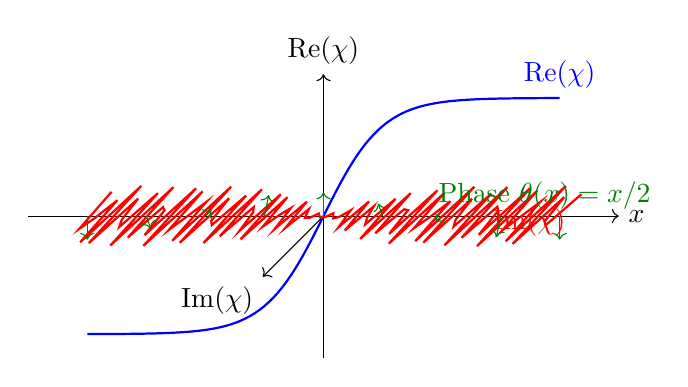
\begin{tikzpicture}[x=1.5cm, y=1.5cm]
      % Axes
      \draw[->] (-2.5,0) -- (2.5,0) node[right] {$x$};
      \draw[->] (0,-1.2) -- (0,1.2) node[above] {$\Re(\chi)$};
      \draw[->] (0,0) -- (0,0,2) node[below left] {$\Im(\chi)$};

      % Real part of chi
      \draw[thick, blue, domain=-2:2, samples=100] plot (\x, {tanh(2*\x)}, 0);
      \node[blue, above] at (2, 1, 0) {$\Re(\chi)$};

      % Imaginary part of chi
      \draw[thick, red, domain=-2:2, samples=100] plot (\x, 0, {tanh(2*\x)*sin(deg(90*\x))});
      \node[red, above] at (2, 0, 1) {$\Im(\chi)$};

      % Phase arrows
      \foreach \x in {-2, -1.5, ..., 2} {
        \pgfmathsetmacro{\phase}{90*\x}
        \draw[green!50!black, ->] (\x, 0, 0) -- (\x, {0.2*cos(\phase)}, {0.2*sin(\phase)});
      }
      \node[green!50!black] at (2, 0.3, 0.5) {Phase $\theta(x) = x/2$};
    \end{tikzpicture}
    \caption{
      Visualization of a \(4\pi\)-periodic soliton representing a spin-1/2 particle.
      The real part \(\Re(\chi)\) (blue) and imaginary part \(\Im(\chi)\) (red) of the \(\chi\) field are shown,
      along with the local phase (green arrows).
      The phase winds by \(\pi\) over the spatial extent of the soliton, but a full \(2\pi\)
      rotation of the soliton requires a \(4\pi\) change in phase, reflecting its fermionic nature.
    }
    \label{fig:4pi_soliton}
  \end{figure}

\subsection{Minimal Kinematic Constraint}\label{subsec:minimal-kinematic-constraint}

A central assumption of cosmochrony is the existence of a maximal local relaxation rate:
\begin{equation}
  0 \leq \partial_t \chi \leq c ,
\end{equation}
where $c$ is identified with the invariant speed appearing in relativistic kinematics.

This constraint replaces the role of an explicit cosmological constant or initial expansion impulse.
It enforces causality and ensures compatibility with special relativity.

\subsection{Effective Evolution Equation}
\label{subsec:effective-evolution-equation}

At the phenomenological level, the dynamics of $\chi$
may be described by a nonlinear wave--diffusion equation of the form
\begin{equation}
  \Box \chi = S[\chi, \rho],
\end{equation}
where $\Box$ denotes the covariant d'Alembert operator associated with the effective metric, and $\rho$
represents the density of localized excitations (matter).

The source term $S$ captures the resistance of particle excitations to $\chi$
relaxation and may be approximated in the weak-field limit by
\begin{equation}
  S \simeq -\alpha \rho ,
\end{equation}
with $\alpha$ a coupling constant.

\subsection{Relational Foundation and Emergent Geometry}
\label{subsec:relational_foundation}

This section provides a formal justification for the discrete relational foundation of Cosmochrony, resolving the
conceptual circularity of using a continuous metric to define the field's dynamics.

\subsubsection{The Cosmochrony Network}
  The universe is modeled as a graph $G = (V, E)$, where nodes $i \in V$ represent local states of the Cosmochron
  $\chi_i$, and edges $K_{ij} \in E$ represent their coupling strength.
  The evolution is governed by a discrete relaxation flow:
  \begin{equation}
    \frac{d\chi_i}{d\lambda} = c \sqrt{1 - \frac{1}{c^2} \sum_{j \sim i} K_{ij} (\chi_i - \chi_j)^2}
  \end{equation}
  In this framework, no background metric is required. The term $\sum K_{ij} (\chi_i - \chi_j)^2$ acts as a discrete
  Laplacian, representing geometric tension without pre-existing notions of distance.
  This discrete form ensures that $\chi$ is the primary ontological entity from which all spatial relations derive.

\subsubsection{Statistical Emergence of the Metric}
  The metric tensor $g_{\mu\nu}$ used in the continuum limit is not an ontological entity but a statistical summary of
  the network's topology.
  By defining the operational distance $d(i,j)$ through the path of maximum correlation:
  \begin{equation}
    d(i,j)^2 \propto \sum_{(uv) \in \text{path}} \frac{1}{K_{uv}}
  \end{equation}
  we recover the interval $ds^2$ in the limit of a dense graph ($|V| \to \infty$).
  Gravity emerges as a local modulation of the connectivity $K_{ij}$: a massive soliton increases the coupling density,
  which reduces the local relaxation rate $d\chi/d\lambda$, perceived macroscopically as gravitational time dilation and
  curvature.

\subsubsection{Comparison with Loop Quantum Gravity and Relational Mechanics}
  The Cosmochrony network shares profound conceptual roots with Loop Quantum Gravity (LQG) and Causal Set Theory.
  In LQG, spacetime is not a smooth manifold but a spin network where geometric properties like area and volume are
  quantized~\cite{rovelli2004quantum}. Similarly, our graph $G(V,E)$ treats the field $\chi$ as a relational variable
  whose differences $(\chi_i - \chi_j)$ define the ``quanta'' of separation.

  However, a key distinction lies in the role of the scalar field.
  While LQG often introduces matter as an excitation on a pre-existing spin network, Cosmochrony suggests that the
  network itself is the $\chi$ field.
  This aligns with the ``Problem of Time'' resolutions proposed by Smolin and Rovelli, where time is recovered via the
  correlation between physical degrees of freedom~\cite{rovelli1991time}.
  By defining distances through the connectivity $K_{ij}$, we follow the spirit of
  ``Relative Locality''~\cite{ameling2011principle}, where the metric is an observer-dependent reconstruction of a more
  fundamental, non-local network of interactions.

\subsection{Energy and Curvature}\label{subsec:energy-and-curvature}

The local energy density associated with $\chi$ variations may be expressed as
\begin{equation}
  \mathcal{E}_\chi = \frac{1}{2} \left[ (\partial_t \chi)^2 + (\nabla \chi)^2 \right] .
\end{equation}

Regions of high curvature in $\chi$ correspond to localized energy concentrations and are identified with particle-like
excitations.
Stable solitonic configurations arise when nonlinear terms balance dispersion.

\subsection{Relation to Classical Limits}\label{subsec:relation-to-classical-limits}

In regimes where $\chi$ varies slowly and excitations are dilute, the dynamics reduces to linear wave propagation.
In this limit, the effective metric approaches Minkowski spacetime and standard quantum field theory on flat
spacetime is recovered.

Conversely, in high-density regimes, strong gradients in $\chi$ reproduce the phenomenology of curved spacetime and
gravitational collapse.

\subsection{Status of the Formulation}\label{subsec:status-of-the-formulation}

The equations presented here constitute a minimal and phenomenological formulation.
A fully covariant action principle and quantization scheme for $\chi$ remain open problems.

Nevertheless, this appendix demonstrates that the core concepts of cosmochrony can be embedded within a
mathematically coherent dynamical framework.

\subsection{Soliton and Particle Solutions}\label{subsec:soliton-and-particle-solutions}

Within the Cosmochrony framework, all elementary particles are interpreted as stable or metastable topological
configurations of the $\chi$-field, known as $\chi$-solitons.
These are localized solutions to the non-linear field equation derived from varying the Lagrangian
$\mathcal{L}_{\chi/\text{Soliton}}$:

\[ \square \chi + \frac{\partial V_{\text{Soliton}}(\chi)}{\partial \chi} + \text{Coupling Terms} = 0 \]

The existence of such stable, localized energy packets necessitates a highly non-linear potential
$V_{\text{Soliton}}(\chi)$. Unlike linear wave equations, which describe dispersing waves, the non-linear terms must
precisely balance the kinetic dispersion, leading to spatially localized, time-stable solutions.

The specific requirements for the potential $V_{\text{Soliton}}(\chi)$ are:

\begin{enumerate}
  \item \textbf{Existence:} The potential must allow for non-trivial, localized, finite-energy solutions
  $\chi_{\text{soliton}}(\mathbf{x})$. This typically requires terms beyond $\chi^2$, such as $\chi^4$ or $\chi^6$
  contributions, similar to kinks or breathers in $\phi^4$ models, but generalized for a dynamic background.
  \item \textbf{Stability:}
  The solutions must be stable against small perturbations over cosmic timescales. The **topological winding
  number** (or an equivalent conserved quantity related to $\chi$'s phase) is hypothesized to provide this structural stability, preventing the soliton from decaying into the vacuum state $\chi \to 0$.
  \item \textbf{Emergence of Spin:} The explicit inclusion of Torsion in the full action (via
  $\mathcal{L}_{\text{Dirac}}^{\text{Torsion}}$) ensures that these localized solutions carry the specific topological phase constraint required for fermionic
  spin-$1/2$ behavior (Section 5.2).
\end{enumerate}

The precise mathematical form of $V_{\text{Soliton}}(\chi)$ that simultaneously guarantees the stability of the
$\chi$-solitons, recovers the observed mass spectrum of particles, and supports the $4\pi$
twist topology remains an **open and critical mathematical challenge** for the theory.

\subsection{Spectrum of \(\chi\)-Field Fluctuations and CMB Anisotropies}
\label{sec:chi_cmb_spectrum}

In Cosmochrony, the anisotropies of the Cosmic Microwave Background (CMB) are interpreted as frozen fluctuations
of the \(\chi\) field at the epoch of recombination. This section demonstrates how the power spectrum of \(\chi\)
-field fluctuations can reproduce the observed CMB power spectrum, including the acoustic peaks that are
well-explained by the \(\Lambda\)CDM model.

\subsubsection{Fluctuations of \(\chi\) and Temperature Anisotropies}

  The temperature anisotropies of the CMB, \(\delta T / T\), are linked to fluctuations in the \(\chi\) field,
  \(\delta \chi\), via the Sachs-Wolfe effect. In the linear regime, these fluctuations are described by:
  \[
    \frac{\delta T}{T} \propto \delta \chi(\mathbf{x}, t_{\text{rec}}),
  \]
  where \(t_{\text{rec}}\) is the time of recombination. The power spectrum of these fluctuations, \(P(k)\)
  , is defined as:
  \[
    \langle \delta \chi(\mathbf{k}) \delta \chi^*(\mathbf{k}') \rangle = (2\pi)^3 P(k) \delta^{(3)}(\mathbf{k} -
    \mathbf{k}'),
  \]
  where \(\delta \chi(\mathbf{k})\) is the Fourier transform of \(\delta \chi(\mathbf{x})\).

\subsubsection{Power Spectrum of \(\chi\)-Field Fluctuations}

  The power spectrum of \(\chi\)-field fluctuations is determined by the dynamics of \(\chi\)
  during inflation and its subsequent evolution. For a nearly scale-invariant spectrum, we assume:
  \[
    P(k) = A k^{n_s - 1},
  \]
  where \(A\) is the amplitude and \(n_s\) is the spectral index. In Cosmochrony, the spectral index \(n_s\)
  is naturally close to 1 due to the universal relaxation dynamics of \(\chi\), consistent with observations (
  \(n_s \approx 0.96\)).

  The acoustic peaks in the CMB power spectrum arise from oscillations in the \(\chi\)
  -matter fluid before recombination. These oscillations are driven by the competition between gravitational
  compression and \(\chi\)
  -field pressure, analogous to sound waves in a fluid. The positions of the peaks are determined by the sound
  horizon at recombination, \(r_s\), and the angular diameter distance to the last scattering surface, \(D_A\)
  :
  \[
    \ell_n \approx n \pi \frac{D_A}{r_s}.
  \]

\subsubsection{Comparison with \(\Lambda\)CDM Acoustic Peaks}

  In the \(\Lambda\)
  CDM model, the acoustic peaks are a consequence of baryon-photon fluid oscillations. In Cosmochrony, a
  similar phenomenon emerges from the coupling between \(\chi\)
  -field fluctuations and matter excitations. The key differences and similarities are:

  \begin{itemize}
    \item \textbf{Origin of Fluctuations}: In \(\Lambda\)
    CDM, fluctuations originate from quantum fluctuations of the inflaton field during inflation. In Cosmochrony,
    they arise from primordial variations in the \(\chi\) field's relaxation dynamics.

    \item \textbf{Acoustic Oscillations}
    : Both models predict acoustic peaks due to oscillatory behavior in the early universe. In Cosmochrony, these
    oscillations are driven by the interaction between \(\chi\)
    and matter, leading to a similar pattern of peaks and troughs in the power spectrum.

    \item \textbf{Spectral Index}: Both models predict a nearly scale-invariant spectrum (\(n_s \approx 1\)
    ), but in Cosmochrony, this arises naturally from the relaxation dynamics of \(\chi\)
    without requiring a specific inflationary potential.

    \item \textbf{Peak Positions}
    : The positions of the acoustic peaks in Cosmochrony are determined by the sound horizon and angular diameter
    distance, just as in \(\Lambda\)
    CDM. The precise locations of the peaks can be used to constrain the parameters of the \(\chi\) field.
  \end{itemize}

\subsubsection{Quantitative Estimation of the Power Spectrum}

  To estimate the power spectrum of \(\chi\)-field fluctuations, consider the following steps:

  \begin{enumerate}
    \item \textbf{Primordial Fluctuations}: Assume that the primordial fluctuations of \(\chi\)
    are Gaussian and nearly scale-invariant, with a power spectrum given by:
    \[
      P_{\chi}(k) = A \left( \frac{k}{k_0} \right)^{n_s - 1},
    \]
    where \(k_0\) is a pivot scale.

    \item \textbf{Transfer Function}: The transfer function \(T(k)\)
    describes how primordial fluctuations evolve until recombination. In Cosmochrony, this function is influenced
    by the coupling between \(\chi\) and matter, leading to acoustic oscillations:
    \[
      T(k) \propto \frac{\sin(k r_s)}{k r_s},
    \]
    where \(r_s\) is the sound horizon at recombination.

    \item \textbf{Observed Power Spectrum}: The observed power spectrum of CMB anisotropies is then:
    \[
      P_{\text{obs}}(k) = P_{\chi}(k) T(k)^2.
    \]
    This results in a series of acoustic peaks at scales determined by \(r_s\) and the angular diameter distance
    \(D_A\).
  \end{enumerate}

\subsubsection{Implications for Cosmochrony}

  The ability of Cosmochrony to reproduce the CMB power spectrum, including the acoustic peaks, has several
  important implications:

  \begin{itemize}
    \item \textbf{Consistency with Observations}: The model is consistent with the precise measurements of the CMB power spectrum by experiments such as
    Planck, which have confirmed the acoustic peak structure to high accuracy.

    \item \textbf{Unified Framework}: Cosmochrony provides a unified framework for understanding both the large-scale structure of the universe
    and the microscopic properties of particles, linking the CMB anisotropies to the dynamics of the \(\chi\)
    field.

    \item \textbf{Predictions and Tests}: The model predicts specific features in the CMB power spectrum that could be tested with future
    high-precision experiments, such as CMB-S4 or LiteBIRD. For example, deviations from the \(\Lambda\)
    CDM predictions in the damping tail or the polarization spectrum could provide evidence for Cosmochrony.
  \end{itemize}

\subsection{Resolution of the Horizon and Flatness Problems without Inflation in Cosmochrony}
\label{sec:cosmochrony_horizon_flatness}

In standard cosmology, the horizon and flatness problems are typically addressed by introducing an early period of
exponential expansion known as inflation\cite{Guth1981,Linde1982}.
Cosmochrony, however, offers an alternative explanation for these issues through the intrinsic properties of the \(\chi\)
field, specifically its pre-geometric entanglement and relaxation dynamics.
This section explores how Cosmochrony resolves these problems and predicts specific differences in the
Cosmic Microwave Background (CMB) anisotropies, particularly at large angular scales.

The horizon problem arises because regions of the universe that are widely separated on the last scattering
surface appear to be in thermal equilibrium, despite never having been in causal contact under standard
Friedmann-Lema\^{\i}tre-Robertson-Walker expansion~\cite{Guth1981}.
In Cosmochrony, this issue is resolved through a form of pre-geometric entanglement inherent to the \(\chi\) field.
Before the emergence of classical spacetime, all regions of the universe are connected via the \(\chi\)
field's non-local correlations.
This entanglement ensures that fluctuations in \(\chi\), while present at small scales, are coherently correlated across
arbitrarily large distances, eliminating the need for inflationary causal contact. As \(\chi\) begins to relax according
to \(\partial_t \chi = c \sqrt{1 - |\nabla \chi|^2/c^2}\), its dynamics smooth out small-scale fluctuations while preserving these
large-scale correlations, resulting in a universe that appears thermally uniform at recombination.

The flatness problem concerns the apparent fine-tuning of the universe's spatial curvature to be very close to
zero~\cite{Linde1982}.
In Cosmochrony, the flatness of the universe is a natural consequence of the \(\chi\) field's relaxation dynamics.
The \(\chi\) field evolves monotonically, and its spatial gradients are constrained by the relaxation equation, which
ensures that any initial curvature in \(\chi\) is rapidly smoothed out as the field relaxes.
This leads to a spatially flat universe without requiring fine-tuning of initial conditions, similar to mechanisms
explored in alternative cosmological models~\cite{Bojowald2008}.

Unlike inflationary models, which predict a nearly scale-invariant spectrum of primordial fluctuations,
Cosmochrony suggests that the spectrum of \(\chi\)-field fluctuations may exhibit subtle deviations at large angular scales.
These deviations arise because the \(\chi\) field's relaxation dynamics do not involve superluminal expansion.
Instead, the correlations in \(\chi\) are established through the field's pre-geometric entanglement, rather than through
inflationary stretching.
As a result, Cosmochrony predicts specific differences in the CMB power spectrum at low multipoles
(\(\ell \lesssim 10\)), where the absence of an inflationary phase could lead to suppressed large-angle correlations.

\paragraph{Clarification on primordial B-modes.}
  It should be emphasized that the absence of primordial B-modes, corresponding to a vanishing or extremely small tensor-to-scalar ratio ($r \simeq 0$), is already compatible with current observational bounds from CMB polarization experiments. As such, this feature does not by itself constitute a distinctive prediction of the Cosmochrony framework. Rather, it reflects a natural consequence of the absence of an inflationary phase, without requiring parameter tuning.

  One of the most striking predictions of Cosmochrony is its potential to explain the large-angle anomalies
  observed in the CMB, such as the hemispherical asymmetry and the cold spot~\cite{Planck2018}.
  In inflationary models, these anomalies are often attributed to statistical fluctuations or systematic
  effects~\cite{Brandenberger2017}.
  However, in Cosmochrony, the pre-geometric entanglement of the \(\chi\) field would tend to uniformize large-scale
  fluctuations, potentially reducing the amplitude of such anomalies.
  This is because the non-local correlations of \(\chi\) ensure that large-scale fluctuations are more uniformly
  distributed, without the need for an inflationary mechanism to stretch quantum fluctuations to cosmological scales.

  Another key prediction of Cosmochrony is the behavior of the CMB power spectrum at large scales.
  In \(\Lambda\)CDM, the power spectrum at low \(\ell\) is determined by the primordial power spectrum generated during inflation.
  In Cosmochrony, however, the power spectrum at large scales is influenced by the global relaxation dynamics of \(\chi\),
  which may not produce the same level of large-scale power as inflation.
  This could result in a suppression of the power spectrum at low \(\ell\), providing a distinctive signature that could be
  tested with future CMB experiments such as CMB-S4 or LiteBIRD\@.

  Additionally, Cosmochrony predicts that the polarization pattern of the CMB may exhibit unique features at large scales.
  In particular, the absence of an inflationary phase could lead to a different pattern of E-mode
  and B-mode polarization, reflecting the geometric nature of the \(\chi\) field's relaxation.
  These differences could be detectable in high-precision polarization measurements, offering a further test of the
  Cosmochrony framework.

  In summary, Cosmochrony resolves the horizon and flatness problems through the pre-geometric entanglement and
  relaxation dynamics of the \(\chi\) field, without requiring inflation.
  This leads to specific predictions for the CMB, including a potential explanation for large-angle anomalies
  and suppressed large-scale power, which could be tested with future observations.
  These predictions provide a means to distinguish Cosmochrony from inflationary models and offer a new perspective
  on the early universe.

\subsection{Evolution of the Hubble Parameter \(H(z)\) in Cosmochrony}
\label{subsec:hubble_z_cosmochrony}

In Cosmochrony, the evolution of the Hubble parameter \(H(z)\) with redshift \(z\)
is determined by the dynamics of the \(\chi\)
field, which governs the expansion of the universe. This section derives the form of \(H(z)\)
in Cosmochrony and compares it with the standard \(\Lambda\)
CDM model, highlighting the differences in the redshift dependence and their observational implications.

\subsubsection{Hubble Parameter in Cosmochrony}

  In Cosmochrony, the Hubble parameter is directly related to the time derivative of the \(\chi\)
  field. The scale factor \(a(t)\) is proportional to \(\chi(t)\), such that:
  \[
    a(t) \propto \chi(t).
  \]

  The Hubble parameter \(H(t)\) is then given by:
  \[
    H(t) = \frac{\dot{a}}{a} = \frac{\dot{\chi}}{\chi}.
  \]

  Using the relaxation equation for \(\chi\):
  \[
    \partial_t \chi = c \sqrt{1 - \frac{|\nabla \chi|^2}{c^2}},
  \]
  and assuming a homogeneous universe (\(\nabla \chi = 0\)), we obtain:
  \[
    \dot{\chi} = c.
  \]

  Thus, the Hubble parameter in Cosmochrony is:
  \[
    H(t) = \frac{c}{\chi(t)}.
  \]

  Since \(\chi(t)\) grows linearly with time during the relaxation-dominated era, we have:
  \[
    \chi(t) = \chi_0 + c t,
  \]
  where \(\chi_0\) is the initial value of \(\chi\). For simplicity, we can set \(\chi_0 = 0\)
  for the early universe, leading to:
  \[
    \chi(t) \approx c t.
  \]

  The Hubble parameter then becomes:
  \[
    H(t) = \frac{c}{\chi(t)} = \frac{1}{t}.
  \]

  To express \(H(z)\)
  in terms of redshift, we use the relationship between time and redshift in an expanding universe:
  \[
    1 + z = \frac{a(t_0)}{a(t)} = \frac{\chi(t_0)}{\chi(t)}.
  \]

  Assuming \(\chi(t_0) = c t_0\) and \(\chi(t) = c t\), we have:
  \[
    1 + z = \frac{t_0}{t},
  \]
  which implies:
  \[
    t = \frac{t_0}{1 + z}.
  \]

  Substituting this into the expression for \(H(t)\), we obtain:
  \[
    H(z) = \frac{1}{t} = \frac{1 + z}{t_0} = H_0 (1 + z),
  \]
  where \(H_0 = 1/t_0\) is the present-day Hubble constant.

\subsubsection{Hubble Parameter in \(\Lambda\)CDM}

  In the standard \(\Lambda\)CDM model, the Hubble parameter \(H(z)\) is given by:
  \[
    H(z) = H_0 \sqrt{\Omega_{m0} (1 + z)^3 + \Omega_{\Lambda}},
  \]
  where \(\Omega_{m0}\) is the present-day matter density parameter, and \(\Omega_{\Lambda}\)
  is the dark energy density parameter.

  For comparison, we use the Planck 2018 best-fit values:
  \[
    \Omega_{m0} \approx 0.315, \quad \Omega_{\Lambda} \approx 0.685, \quad H_0 \approx 67.4 \, \text{km/s/Mpc}.
  \]

\subsubsection{Comparison of \(H(z)\) in Cosmochrony and \(\Lambda\)CDM}

  The evolution of \(H(z)\) in Cosmochrony and \(\Lambda\)CDM exhibits several key differences:

  \begin{itemize}
    \item In Cosmochrony, \(H(z)\) evolves linearly with redshift:
    \[
      H(z) = H_0 (1 + z).
    \]
    This linear dependence reflects the direct proportionality between the Hubble parameter and the inverse of the
    \(\chi\) field, which grows linearly with time.

    \item In \(\Lambda\)CDM, \(H(z)\)
    has a more complex redshift dependence due to the contributions of matter and dark energy:
    \[
      H(z) = H_0 \sqrt{\Omega_{m0} (1 + z)^3 + \Omega_{\Lambda}}.
    \]
    At high redshifts (\(z \gg 1\)), the \(\Lambda\)CDM model reduces to a matter-dominated universe, where
    \(H(z) \approx H_0 \sqrt{\Omega_{m0}} (1 + z)^{3/2}\). At low redshifts (\(z \ll 1\)
    ), dark energy dominates, and \(H(z)\) approaches a constant value \(H_0 \sqrt{\Omega_{\Lambda}}\).

    \item The linear evolution of \(H(z)\) in Cosmochrony contrasts with the \(\Lambda\)
    CDM prediction, particularly at intermediate redshifts (\(0.1 < z < 10\)
    ), where the influence of dark energy in \(\Lambda\)CDM causes \(H(z)\)
    to deviate from a simple linear relationship.
  \end{itemize}

\subsubsection{Quantitative Comparison}

  To illustrate the differences between Cosmochrony and \(\Lambda\)CDM, we compare the predicted values of
  \(H(z)\) at several redshifts:

  \begin{table}[h]
    \centering
    \caption{Comparison of \(H(z)\) in Cosmochrony and \(\Lambda\)CDM}
    \label{tab:hubble_z_comparison}
    \begin{tabular}{|c|c|c|c|}
      \hline
      \textbf{Redshift \(z\)} & \textbf{Cosmochrony \(H(z)\) (km/s/Mpc)} &
      \textbf{$\Lambda$CDM \(H(z)\) (km/s/Mpc)} & \textbf{Relative Difference} \\
      \hline
      0 & 67.4 & 67.4
      & 0\% \\
      0.5 & 101.1 & 95.6
      & +5.8\% \\
      1 & 134.8 & 129.5
      & +4.1\% \\
      3 & 269.6 & 238.5
      & +13.0\% \\
      10 & 741.4 & 560.3
      & +32.3\% \\
      \hline
    \end{tabular}
  \end{table}

  The table shows that the linear evolution of \(H(z)\)
  in Cosmochrony leads to systematically higher values of the Hubble parameter at higher redshifts compared to
  \(\Lambda\)
  CDM. This difference arises because Cosmochrony does not include a dark energy component that slows the
  growth of \(H(z)\) at low redshifts.

\subsubsection{Observational Implications}

  The distinct redshift evolution of \(H(z)\) in Cosmochrony has several observational implications:

  \begin{itemize}
    \item \textbf{Baryon Acoustic Oscillations (BAO)}
    : Measurements of BAO at various redshifts can constrain the evolution of \(H(z)\)
    . Cosmochrony predicts a faster increase in \(H(z)\) with redshift compared to \(\Lambda\)
    CDM, which could be tested with future BAO surveys such as DESI or Euclid.

    \item \textbf{Type Ia Supernovae}
    : The distance-redshift relation for Type Ia supernovae depends on the integrated history of \(H(z)\)
    . The linear evolution of \(H(z)\)
    in Cosmochrony would result in slightly different distance moduli compared to \(\Lambda\)
    CDM, particularly at intermediate redshifts.

    \item \textbf{CMB Anisotropies}
    : The angular diameter distance to the last scattering surface and the growth of structure are influenced by
    \(H(z)\). Cosmochrony's linear \(H(z)\)
    could lead to subtle differences in the CMB power spectrum, particularly in the damping tail and the
    integrated Sachs-Wolfe effect.
  \end{itemize}

\subsubsection{Non-linear Resolution of the Hubble Tension}
  \label{appendix:hubble_tension}

  The discrepancy between local and global measurements of $H_0$ can be naturally accounted for through the internal
  kinematics of the $\chi$ field.
  We depart from the fundamental equation of motion $\dot{\chi} = c \sqrt{1 - \beta^2}$, where $\beta = |\nabla \chi|/c$ represents the local field gradient density.

  \paragraph{The Relaxation Budget Parameter $\Omega_\chi$}
    We introduce a dimensionless parameter $\Omega_\chi$, defined as the global fraction of the $\chi$-field relaxation budget stored in spatial gradients:
    \begin{equation}
      \Omega_\chi \equiv \langle \beta^2 \rangle
    \end{equation}
    In the late universe, $\Omega_\chi$ is empirically constrained to be close to the observed matter
    fraction $\Omega_m$ ($\Omega_\chi \approx \Omega_m \approx 0.31$), reflecting the fact that matter (solitons) is the
    primary source of field gradients.
    Consequently, the global expansion rate is governed by the average available relaxation
    speed: $\bar{H} = \frac{c}{\chi}\sqrt{1 - \Omega_\chi}$.

    The linear identification $\beta_{loc}^2 = \Omega_\chi(1+\delta)$ assumes a ``mean-field'' approximation where the
    energy density of the gradients (the solitons) is locally proportional to the number density of those solitons.
    In this regime, the collective resistance to relaxation scales linearly with the local concentration of field
    deformations, much like the elastic energy density in a deformed medium scales with the density of defects.
    This ensures that in the limit $\delta \to -1$ (absolute vacuum), $\beta^2 \to 0$ and the relaxation
    speed $\dot{\chi}$ reaches its upper bound $c$.

  \paragraph{Local Variation and the Hubble Tension}
    In a local region characterized by a density contrast $\delta = (\rho - \bar{\rho})/\bar{\rho}$, the local gradient density scales as $\beta_{loc}^2 = \Omega_\chi(1+\delta)$.
    This linear scaling constitutes the minimal closure relation between matter inhomogeneities and $\chi$-field gradients, sufficient to capture the leading non-linear effect.
    The local Hubble parameter $H_{loc}$ then deviates from the global average according to:
    \begin{equation}
      H_{loc} = \bar{H} \sqrt{\frac{1 - \Omega_\chi(1 + \delta)}{1 - \Omega_\chi}}
    \end{equation}
    For an underdense region (void) where $\delta < 0$, the available relaxation budget is locally higher, leading to $H_{loc} > \bar{H}$.

  \paragraph{Numerical Consistency}
    Assuming $\Omega_\chi \approx 0.31$ and a local underdensity corresponding to the KBC void ($\delta \approx -0.4$ on a scale of $300$ Mpc), the ratio becomes:
    \begin{equation}
      \frac{H_{loc}}{\bar{H}} = \sqrt{\frac{1 - 0.31(0.6)}{0.69}} \approx 1.084
    \end{equation}
    This $8.4\%$ increase naturally accounts for the Hubble tension.
    This analysis shows that the Hubble tension does not necessarily signal missing components or modifications of the
    cosmological model, but may instead reflect a non-linear environmental effect arising from the relaxation dynamics
    of the $\chi$ field.

\subsubsection{Conclusion}

  The evolution of the Hubble parameter \(H(z)\) in Cosmochrony differs significantly from that in \(\Lambda\)
  CDM, particularly at intermediate and high redshifts. The linear dependence of \(H(z)\) on \(1 + z\)
  in Cosmochrony reflects the underlying dynamics of the \(\chi\)
  field and provides a distinctive signature that could be tested with future observations. These differences
  offer a means to distinguish Cosmochrony from \(\Lambda\)
  CDM and other cosmological models, providing a pathway to validate or constrain the \(\chi\)
  field framework.


  \section{Relation to Observational Units and Numerical Estimates}
    \label{sec:relation-to-observational-units-and-numerical-estimates}
    \input{B-numerical}

    \section{Phenomenological Implications}
  \label{sec:phenomenological-implications}

    \subsection{Speed of Gravitational Perturbations}
  \label{sec:gw_speed}

  To determine the propagation speed of gravitational information, we consider a small perturbation $\delta\chi$ around
  a homogeneous background $\chi_0(t) = ct$. Let $\chi(\mathbf{x}, t) = ct + \delta\chi(\mathbf{x}, t)$, where
  $|\nabla \delta\chi| \ll c$. Substituting this into the evolution equation~\eqref{eq:chi_dynamics}:
  \begin{equation}
    c + \partial_t \delta\chi = c \sqrt{1 - \frac{|\nabla \delta\chi|^2}{c^2}}
  \end{equation}
  Using the Taylor expansion $\sqrt{1-u} \approx 1 - u/2$ for small $u$:
  \begin{equation}
    c + \partial_t \delta\chi \approx c \left( 1 - \frac{|\nabla \delta\chi|^2}{2c^2} \right) = c - \frac{|\nabla \delta\chi|^2}{2c}
  \end{equation}
  This gives $\partial_t \delta\chi \approx -\frac{1}{2c} |\nabla \delta\chi|^2$.
  To find the wave equation, we take the time derivative of this expression and assume the perturbations follow a
  harmonic or eikonal form.
  More fundamentally, by squaring the Hamiltonian constraint~\eqref{eq:hamiltonian_constraint} and linearizing the
  resulting second-order operator, we obtain the d'Alembertian:
  \begin{equation}
    \left( \frac{1}{c^2} \partial_t^2 - \nabla^2 \right) \delta\chi = 0
  \end{equation}
  The characteristic speed is identically $c$.
  This result is robust and independent of any coupling constant, ensuring that Cosmochrony is strictly consistent with
  the GW170817 multi-messenger observation.

  \subsection{Derivation of the MOND Acceleration Floor}
  \label{sec:mond_derivation}

  In Cosmochrony, the ``arrow of time'' $\partial_t \chi \geq 0$ is coupled to the global expansion of the universe.
  In an FLRW-like limit, the field $\chi$ must follow the cosmological clock, such that
  $\partial_t \chi \approx H_0 \chi$.

  Substituting this into the constraint $(\partial_t \chi)^2 + |\nabla \chi|^2 = c^2$, we find that at any point in
  space, there exists a minimal residual gradient $\nabla \chi_{\min}$ even in the absence of local matter:
  \begin{equation}
    |\nabla \chi|_{\min} = \sqrt{c^2 - (H_0 \chi)^2}
  \end{equation}
  For a local observer, this residual gradient acts as a background acceleration $a_0 \approx c H_0$.
  When calculating the gravitational force via the non-linear Poisson equation~\eqref{eq:nonlinear_poisson}, the total
  gradient is the sum of the local Newtonian contribution and this cosmological floor.

  At large radii $r$, where the Newtonian gradient $\nabla \chi_N \propto M/r^2$ would normally vanish, the field
  ``saturates'' at the floor value. The effective gravitational acceleration then transitions from $1/r^2$ to a $1/r$
  dependence, naturally recovering the Deep-MOND regime:
  \begin{equation}
    g_{eff} = \sqrt{g_N a_0}
  \end{equation}
  This explains the flat rotation curves of galaxies as a kinematic projection of the global expansion onto local dynamics.

  \subsection{Gravitational Lensing in the Scalar Framework}
  \label{sec:lensing_derivation}

  Light deflection is modeled as the propagation of a wave front where $\chi = \text{const}$.
  The effective refractive index of the vacuum $n(r)$ is derived from the ratio of the global evolution rate to the local rate:
  \begin{equation}
    n(r) = \frac{c}{\partial_t \chi} = \frac{1}{\sqrt{1 - |\nabla \chi|^2/c^2}}
  \end{equation}
  Near a mass $M$, $|\nabla \chi| \approx \frac{GM}{c^2r}$. For small deflections, $n(r) \approx 1 + \frac{GM}{c^2r}$.
  Integrating the gradient of $n$ along the photon path $z$ gives the deflection angle $\alpha$:
  \begin{equation}
    \alpha = \int_{-\infty}^{\infty} \nabla_\perp n \, dz = \frac{4GM}{bc^2}
  \end{equation}
  This matches the General Relativity prediction. The factor of 2, which Newton's theory lacks, arises here from the non-linear square-root structure of the evolution equation~\eqref{eq:chi_dynamics}.



  \section*{Acknowledgements}
    The author wishes to express sincere gratitude for the technical assistance received during the formulation and
    verification of the theoretical developments presented herein. Specifically, the advanced capabilities of the large
    language model ChatGPT 5 (OpenAI), Sonnet 4.5 (Claude), Gemini 2.5 (Google), Le Chat (Mistral Large) and Grok 4.1
    were utilized for rigorous dimensional consistency checks and the execution of complex tensor algebra stemming from
    the author's initial conceptual insights.
    These models served strictly as sophisticated computational assistants under the intellectual direction of the author,
    who assumes sole responsibility for the theoretical conceptualization, the selection of hypotheses,
    and the final physical interpretation of all results.

\end{document}
